\documentclass[conference,a4paper]{IEEEtran}
\usepackage{graphicx,amsmath,amssymb,array,cite,float}
\usepackage[hidelinks]{hyperref}
\raggedbottom   % no stretched gaps between pinned figures
\begin{document}
\onecolumn
{\small\tableofcontents}
\clearpage
\twocolumn
\title{VLSI Design Course Project\\Designing and Implementing a 4-bit CLA and a SIMD-Reconfigurable 8-bit Adder}
\author{\IEEEauthorblockN{Bhargav}
\IEEEauthorblockA{2025102061\\IIIT Hyderabad\\Draft 1: Parts I and II}}
\maketitle
\begin{abstract}
This project designs a 4-bit carry look-ahead adder (CLA) in TSMC 180\,nm, then joins two copies into a SIMD-reconfigurable 8-bit adder. The 4-bit adder uses a static CMOS prefix carry tree with OR-type transmit and dual-rail AOI22 sums, registered by TSPC flip-flops. Every gate, block and full circuit is simulated in NGSPICE before and after layout in MAGIC. The worst case is found by searching all single-input transitions rather than assumed: post-layout, the 4-bit adder's worst delay is 579.88 ps and the registered circuit works up to 1.147 GHz. In the 8-bit adder, a NAND2-and-inverter carry-gating cell switches between one 8-bit and two 4-bit additions, at a post-layout cost of 7.56\% in carry delay and 1.50\% in power.
\end{abstract}
\section{Introduction}
Addition is the core of every datapath. A ripple-carry adder passes the carry from bit to bit, so the top sum bit waits for every lower bit and the delay grows with word length. A carry look-ahead adder (CLA) computes every carry from generate and propagate signals in parallel, so no carry waits for the one below it.

This project designs a registered 4-bit CLA in TSMC 180\,nm (Part I), then joins two copies into an 8-bit adder that can be reconfigured into two independent 4-bit adders with one control signal (Part II). The primary objective throughout is the smallest \emph{post-layout worst-case delay}; area and power are reported as trade-offs. Inputs are captured by D flip-flops on a rising clock edge and the result is captured on the next rising edge. Every output drives a $W_p/W_n = 20\lambda/10\lambda$ inverter, $\lambda = 0.09\,\mu$m, $V_{DD} = 1.8$\,V.

All simulations use NGSPICE with the provided model; all layouts use MAGIC with the provided SCN6M\_DEEP technology file. Every plot carries the title format \texttt{Name-Roll-question-part}, as the course asks.

\section{Design Proposal}
\begin{itemize}
\item $V_{DD} = 1.8$\,V, technology TSMC 180\,nm, $L_n = L_p = 2\lambda$.
\item Logic style: static CMOS for every adder gate; TSPC dynamic flip-flops.
\end{itemize}
\subsection{Generate, Propagate, Carry and Sum}
For bits $a_i$ and $b_i$:
\[ g_i = a_i b_i, \qquad p_i = a_i \oplus b_i, \]
\[ c_{i+1} = g_i + p_i c_i, \qquad s_i = p_i \oplus c_i . \]
Expanding the carry rule removes the ripple:
\begin{align*}
c_1 &= g_0 + p_0 c_0\\
c_2 &= g_1 + p_1 g_0 + p_1 p_0 c_0\\
c_3 &= g_2 + p_2 g_1 + p_2 p_1 g_0 + p_2 p_1 p_0 c_0\\
c_4 &= g_3 + p_3 g_2 + p_3 p_2 g_1 + p_3 p_2 p_1 g_0 + p_3 p_2 p_1 p_0 c_0
\end{align*}
Built directly, $c_4$ needs a five-input AND term, so a five-transistor stack, and $c_0$ fans out to every carry gate. Both make the circuit slow.

\subsection{Optimization}
\textbf{OR-type transmit.} In the carry terms, $p_i$ can be replaced by $t_i = a_i + b_i$. The two differ only when $a_i = b_i = 1$, and then $g_i = 1$ already sets the carry. A NOR2 gives $\overline{t_i}$ in one light stage, and XOR is kept only for the sum. The idea follows Miao and Li~\cite{miao}.

\textbf{Prefix carry tree.} Bits are merged two at a time into group signals, and $c_0$ is added last:
\[ G_{1:0} = g_1 + t_1 g_0, \quad T_{1:0} = t_1 t_0, \]
\[ G_{3:0} = G_{3:2} + T_{3:2}\,G_{1:0}, \quad G_{2:0} = g_2 + t_2\,G_{1:0}, \]
\[ c_k = G_{k-1:0} + T_{k-1:0}\, c_0 . \]
No gate has more than two transistors in series, and $c_0$ reaches each carry through one inverter and one gate.

\begin{table}[H]\centering\footnotesize
\caption{Unit-size comparison of six candidate architectures, schematic, worst over all 4608 single-input transitions}
\begin{tabular}{|c|c|c|c|}\hline
Candidate & T & Worst (ps) & Hint vector (ps) \\ \hline
C1 & 208 & 771.3 & 421.4 \\ \hline
C2 & 170 & 764.0 & 577.2 \\ \hline
R & 172 & 727.0 & 574.2 \\ \hline
C3 & 170 & 796.4 & 623.5 \\ \hline
C4 & 194 & 658.9 & 360.0 \\ \hline
E & 144 & 799.8 & 629.1 \\ \hline
\end{tabular}
\end{table}

C1 is the textbook XOR and NAND-NAND design, C2 one complex gate per carry, R C2 with a mirror gate for $c_4$, C3 a design with stacks limited to 3, C4 the prefix tree, and E a static Manchester chain. C4 was fastest, so it was chosen. Only the chosen design is taken to the post-layout results below. The six designs differ only in their carry logic.

\section{Design Details}

\begin{figure*}[!t]\centering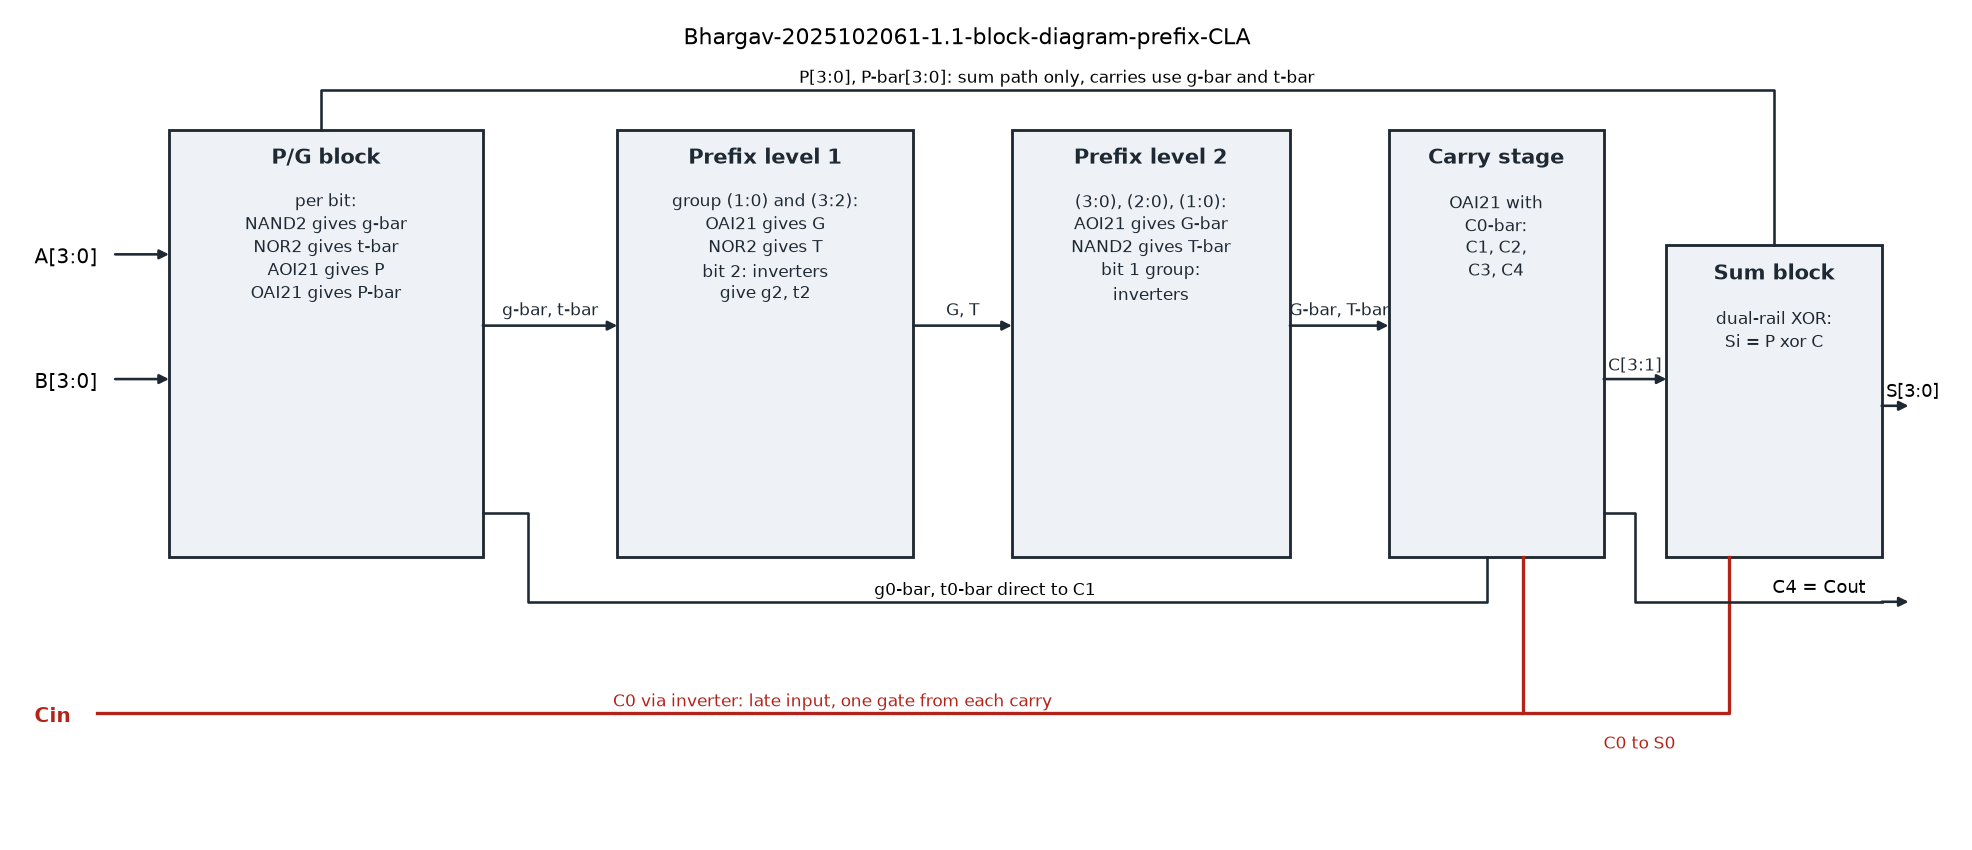
\includegraphics[width=0.92\textwidth]{figures/figures_block_diagram.png}\caption{Block-level architecture of the 4-bit CLA.}\end{figure*}

\textbf{Blocks.} Each bit has a P/G front end: NAND2 gives $\overline{g_i}$, NOR2 gives $\overline{t_i}$, and two compound gates reuse them to make $p_i$ (AOI21) and $\overline{p_i}$ (OAI21). The carry block is the prefix tree: OAI21 and NOR2 for pairs, AOI21 and NAND2 for groups down to bit 0, then one OAI21 per carry with $\overline{c_0}$. The sum is a dual-rail AOI22 XOR, $s_i = \overline{p_i c_i + \overline{p_i}\,\overline{c_i}}$, with an inverter for $\overline{c_i}$.

\textbf{Sizing.} The reference inverter is $W_n = 10\lambda$, $W_p = 20\lambda$. A unit-size gate matches its worst-case pull-up and pull-down resistance to that inverter. The final sizes were found by a search that minimised the worst delay over all transitions, then repeated with wire capacitance taken from the extracted layout. Table~\ref{tab:gatesize} lists the unit cells used in Sections IV and VI; Table~\ref{tab:sizing} lists every instance of the final adder.

\begin{table}[H]\centering\footnotesize
\caption{Unit cell sizes (widths in $\lambda$; several values are different stack positions)}
\label{tab:gatesize}
\begin{tabular}{|c|c|c|c|}\hline
Cell & T & NMOS W & PMOS W \\ \hline
Inverter & 2 & 10 & 20 \\ \hline
NAND2 & 4 & 20 & 20 \\ \hline
NOR2 & 4 & 10 & 40 \\ \hline
AOI21 & 6 & 10/20 & 40 \\ \hline
OAI21 & 6 & 20 & 20/40 \\ \hline
AOI22 XOR (sum) & 10 & 10/20 & 20/40 \\ \hline
\end{tabular}
\end{table}

\begin{table}[H]\centering\scriptsize
\caption{Final adder sizing, every instance (widths in $\lambda$)}
\label{tab:sizing}
\begin{tabular}{|c|c|c|c|c|}\hline
Inst. & Cell & Output & NMOS W & PMOS W \\ \hline
nand0 & nand2 & g0b & 25 & 25 \\ \hline
nor0 & nor2 & t0b & 16 & 62 \\ \hline
aoi0 & aoi21 & p0 & 4/8 & 16 \\ \hline
oai0 & oai21 & p0b & 8 & 8/16 \\ \hline
nand1 & nand2 & g1b & 25 & 25 \\ \hline
nor1 & nor2 & t1b & 20 & 78 \\ \hline
aoi1 & aoi21 & p1 & 4/8 & 16 \\ \hline
oai1 & oai21 & p1b & 8 & 8/16 \\ \hline
nand2 & nand2 & g2b & 25 & 25 \\ \hline
nor2 & nor2 & t2b & 12 & 50 \\ \hline
aoi2 & aoi21 & p2 & 8/16 & 32 \\ \hline
oai2 & oai21 & p2b & 16 & 16/32 \\ \hline
nand3 & nand2 & g3b & 20 & 20 \\ \hline
nor3 & nor2 & t3b & 12 & 50 \\ \hline
aoi3 & aoi21 & p3 & 10/20 & 40 \\ \hline
oai3 & oai21 & p3b & 20 & 20/40 \\ \hline
invc0 & inv & c0b & 10 & 20 \\ \hline
g10 & oai21\_fn & g1\_0 & 25 & 25/50 \\ \hline
t10 & nor2 & t1\_0 & 16 & 62 \\ \hline
g32 & oai21 & g3\_2 & 16 & 16/32 \\ \hline
t32 & nor2 & t3\_2 & 8 & 32 \\ \hline
ig2 & inv & g2 & 12 & 25 \\ \hline
it2 & inv & t2 & 20 & 39 \\ \hline
g30 & aoi21\_fnp & g3\_0b & 4/8 & 16 \\ \hline
t30 & nand2 & t3\_0b & 8 & 8 \\ \hline
g20 & aoi21\_fnp & g2\_0b & 10/20 & 40 \\ \hline
t20 & nand2 & t2\_0b & 25 & 25 \\ \hline
ig10 & inv & g1\_0b & 10 & 20 \\ \hline
it10 & inv & t1\_0b & 16 & 31 \\ \hline
c1 & oai21 & c1 & 10 & 10/20 \\ \hline
c2 & oai21\_fn & c2 & 25 & 25/50 \\ \hline
c3 & oai21\_fn & c3 & 25 & 25/50 \\ \hline
c4g & oai21\_fnp & c4 & 16 & 16/32 \\ \hline
x0 & xor\_aoi22 & s0 & 5/25 & 10/50 \\ \hline
x1 & xor\_aoi22 & s1 & 6/20 & 13/40 \\ \hline
x2 & xor\_aoi22 & s2 & 12/16 & 25/32 \\ \hline
x3 & xor\_aoi22 & s3 & 10 & 20 \\ \hline
\end{tabular}
\end{table}

\textbf{D flip-flop.} A true single-phase clock (TSPC) flip-flop~\cite{yuan} needs one clock and 11 transistors. At a 15\,fF load it gave clock-to-Q plus setup of 212.9\,ps, against 316.8\,ps for a 22-transistor transmission-gate master-slave flip-flop, so TSPC was chosen.

\begin{figure*}[!t]\centering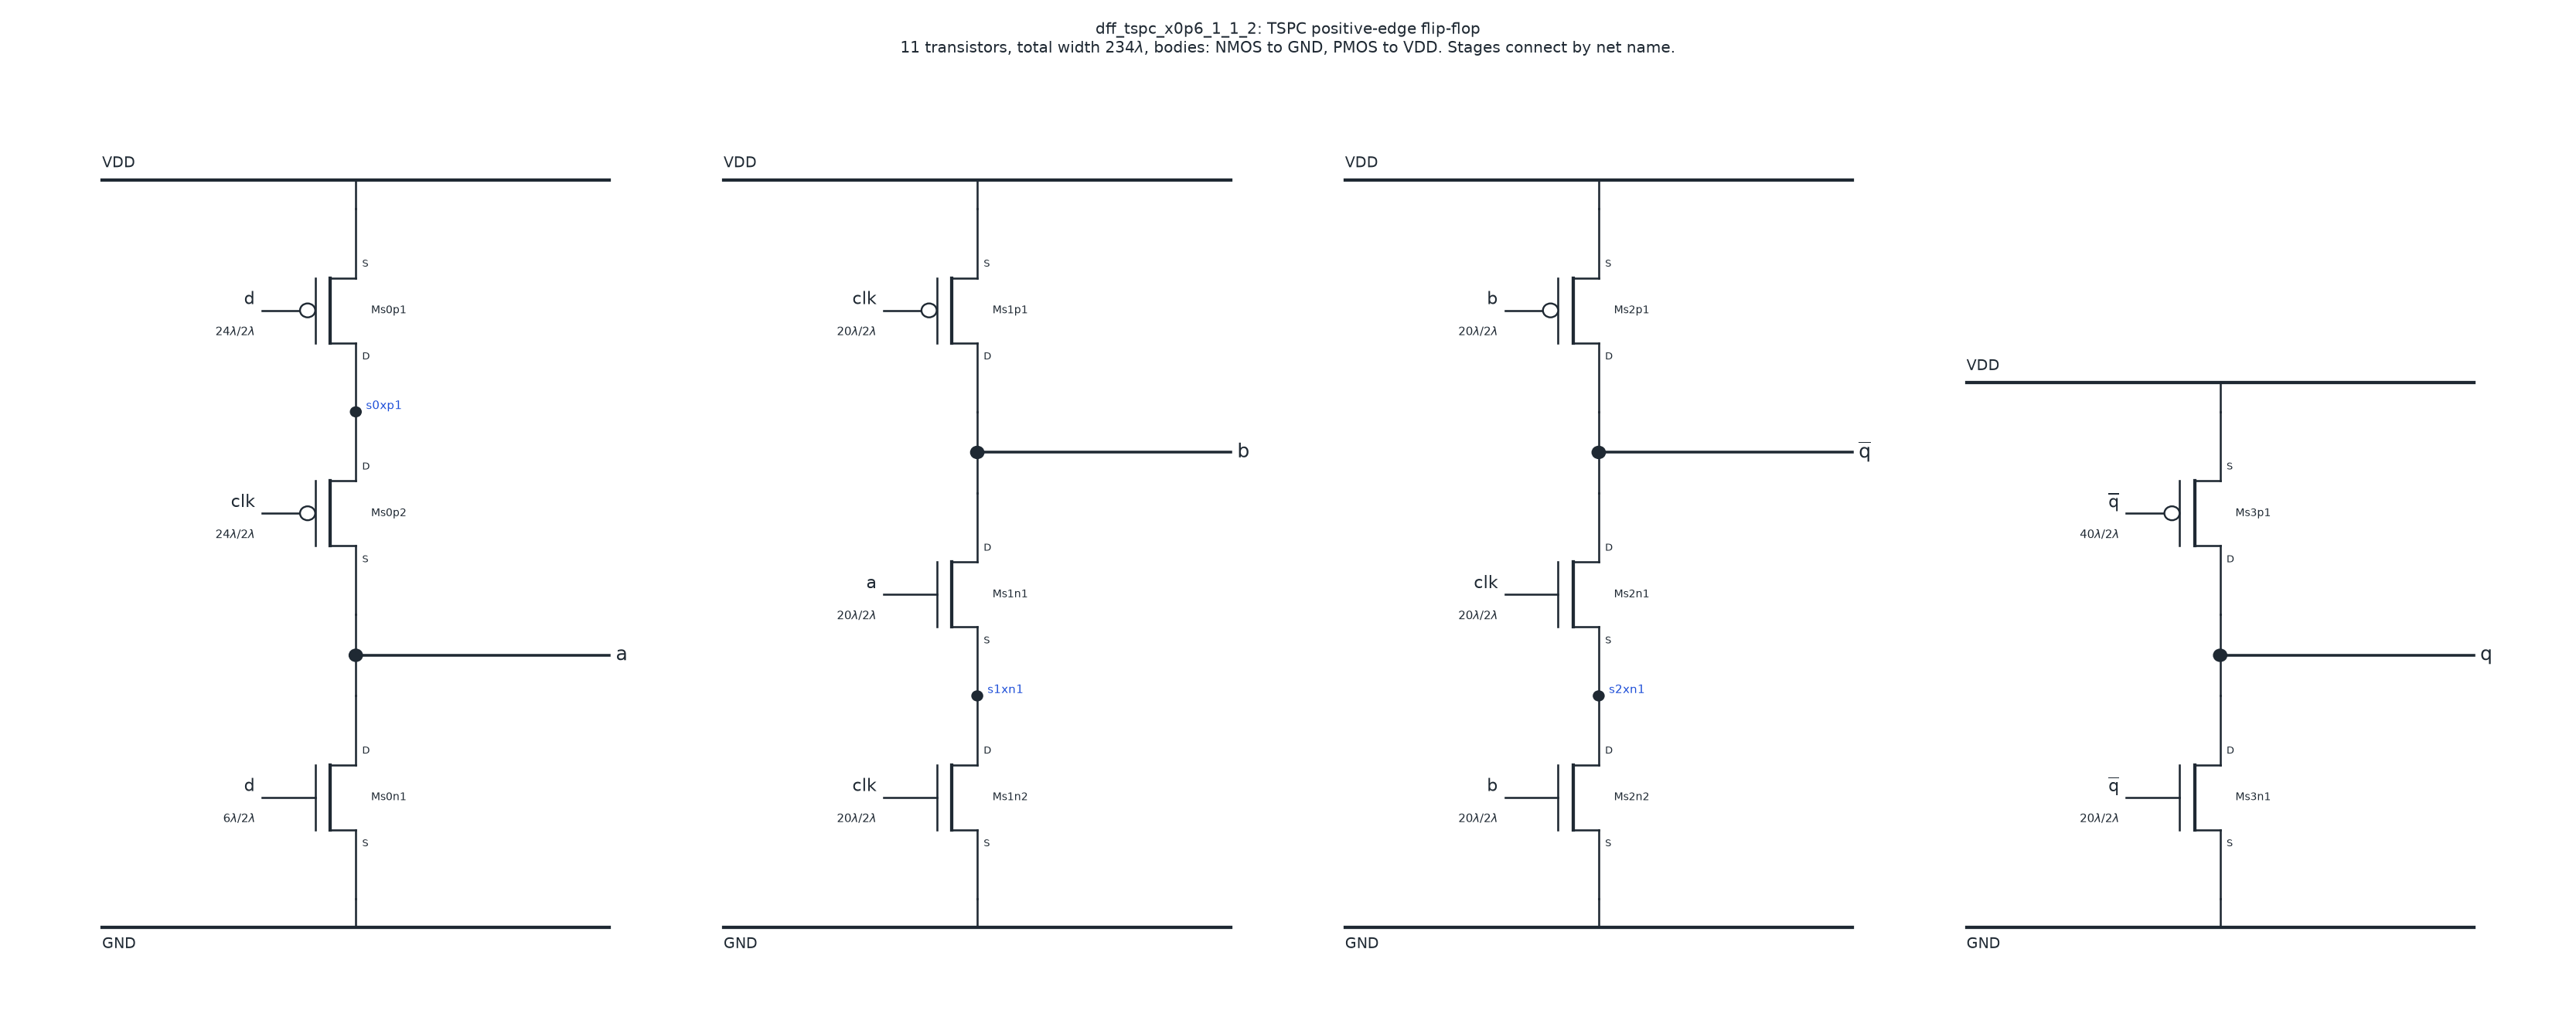
\includegraphics[width=0.85\textwidth]{figures/final_dff_final.png}\caption{TSPC flip-flop, stage drives x0.6, x1, x1, x2, sized at the largest adder input load of 47.76 fF.}\label{fig:dffsch}\end{figure*}

\begin{figure}[H]\centering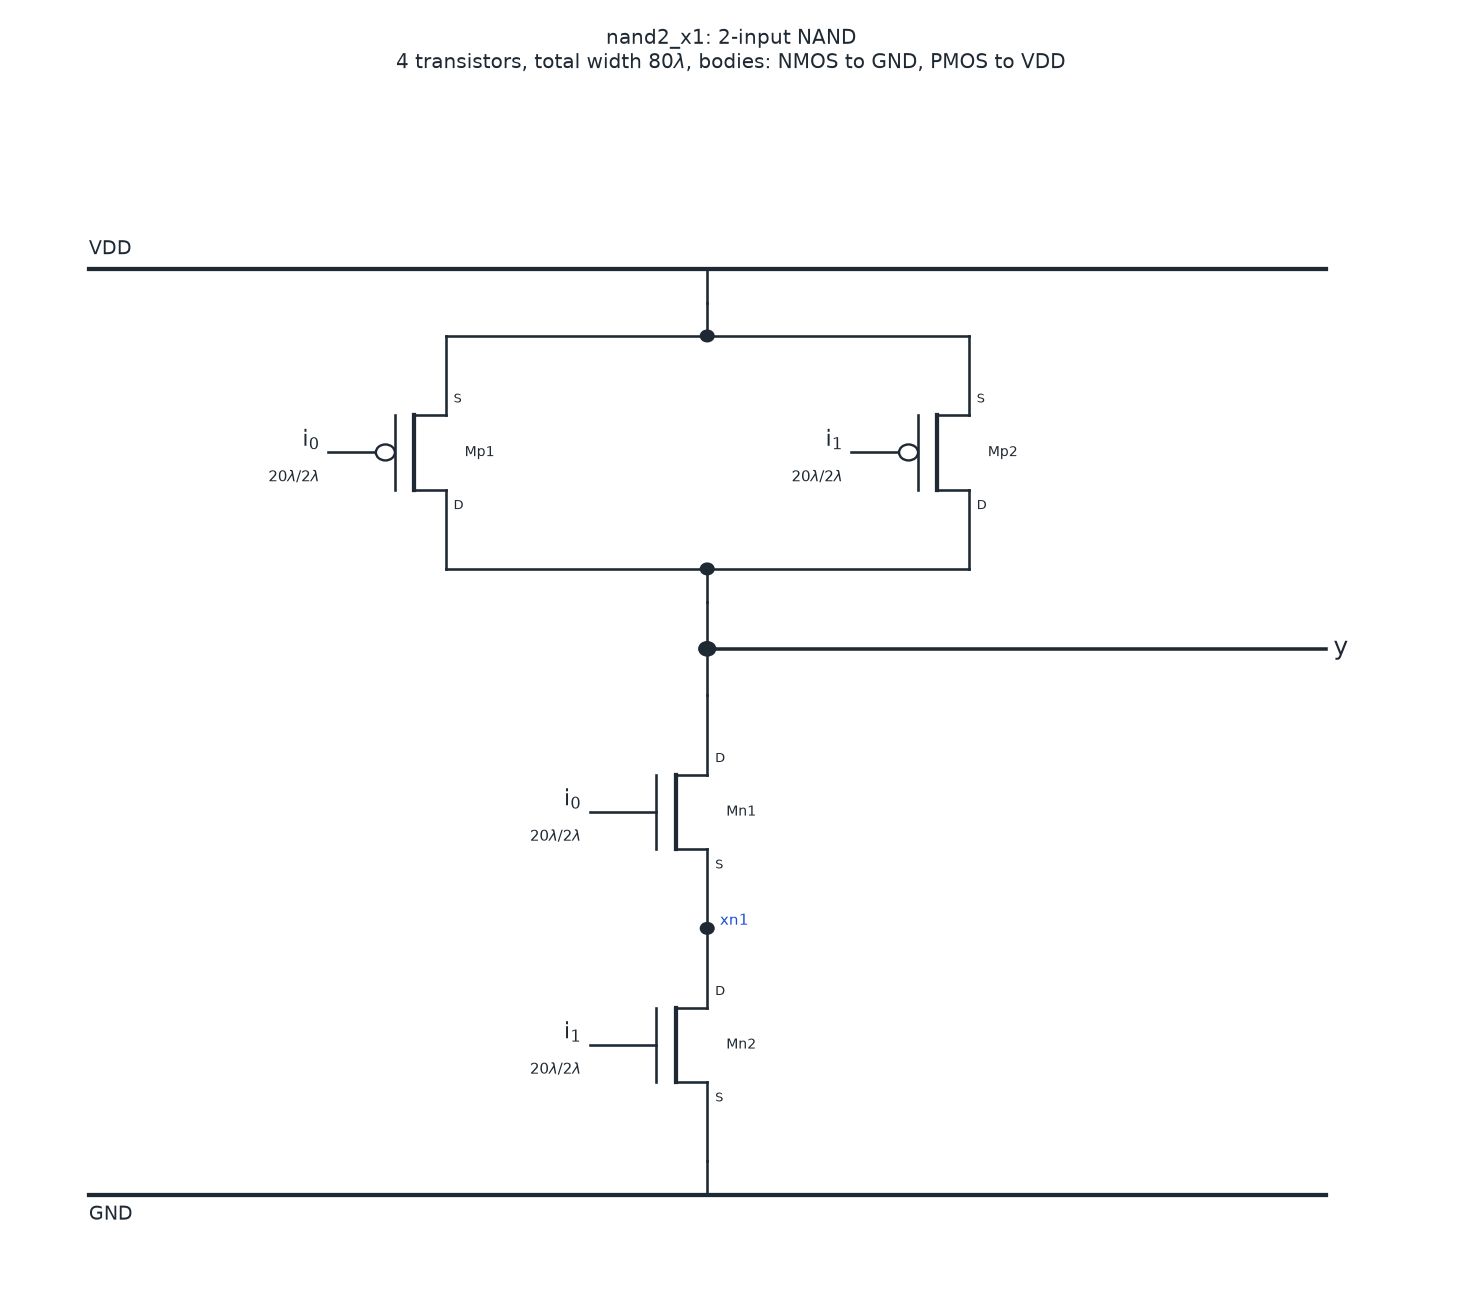
\includegraphics[width=0.8\columnwidth]{figures/final_nand2_x1.png}\caption{Transistor schematic: NAND2.}\end{figure}

\begin{figure}[H]\centering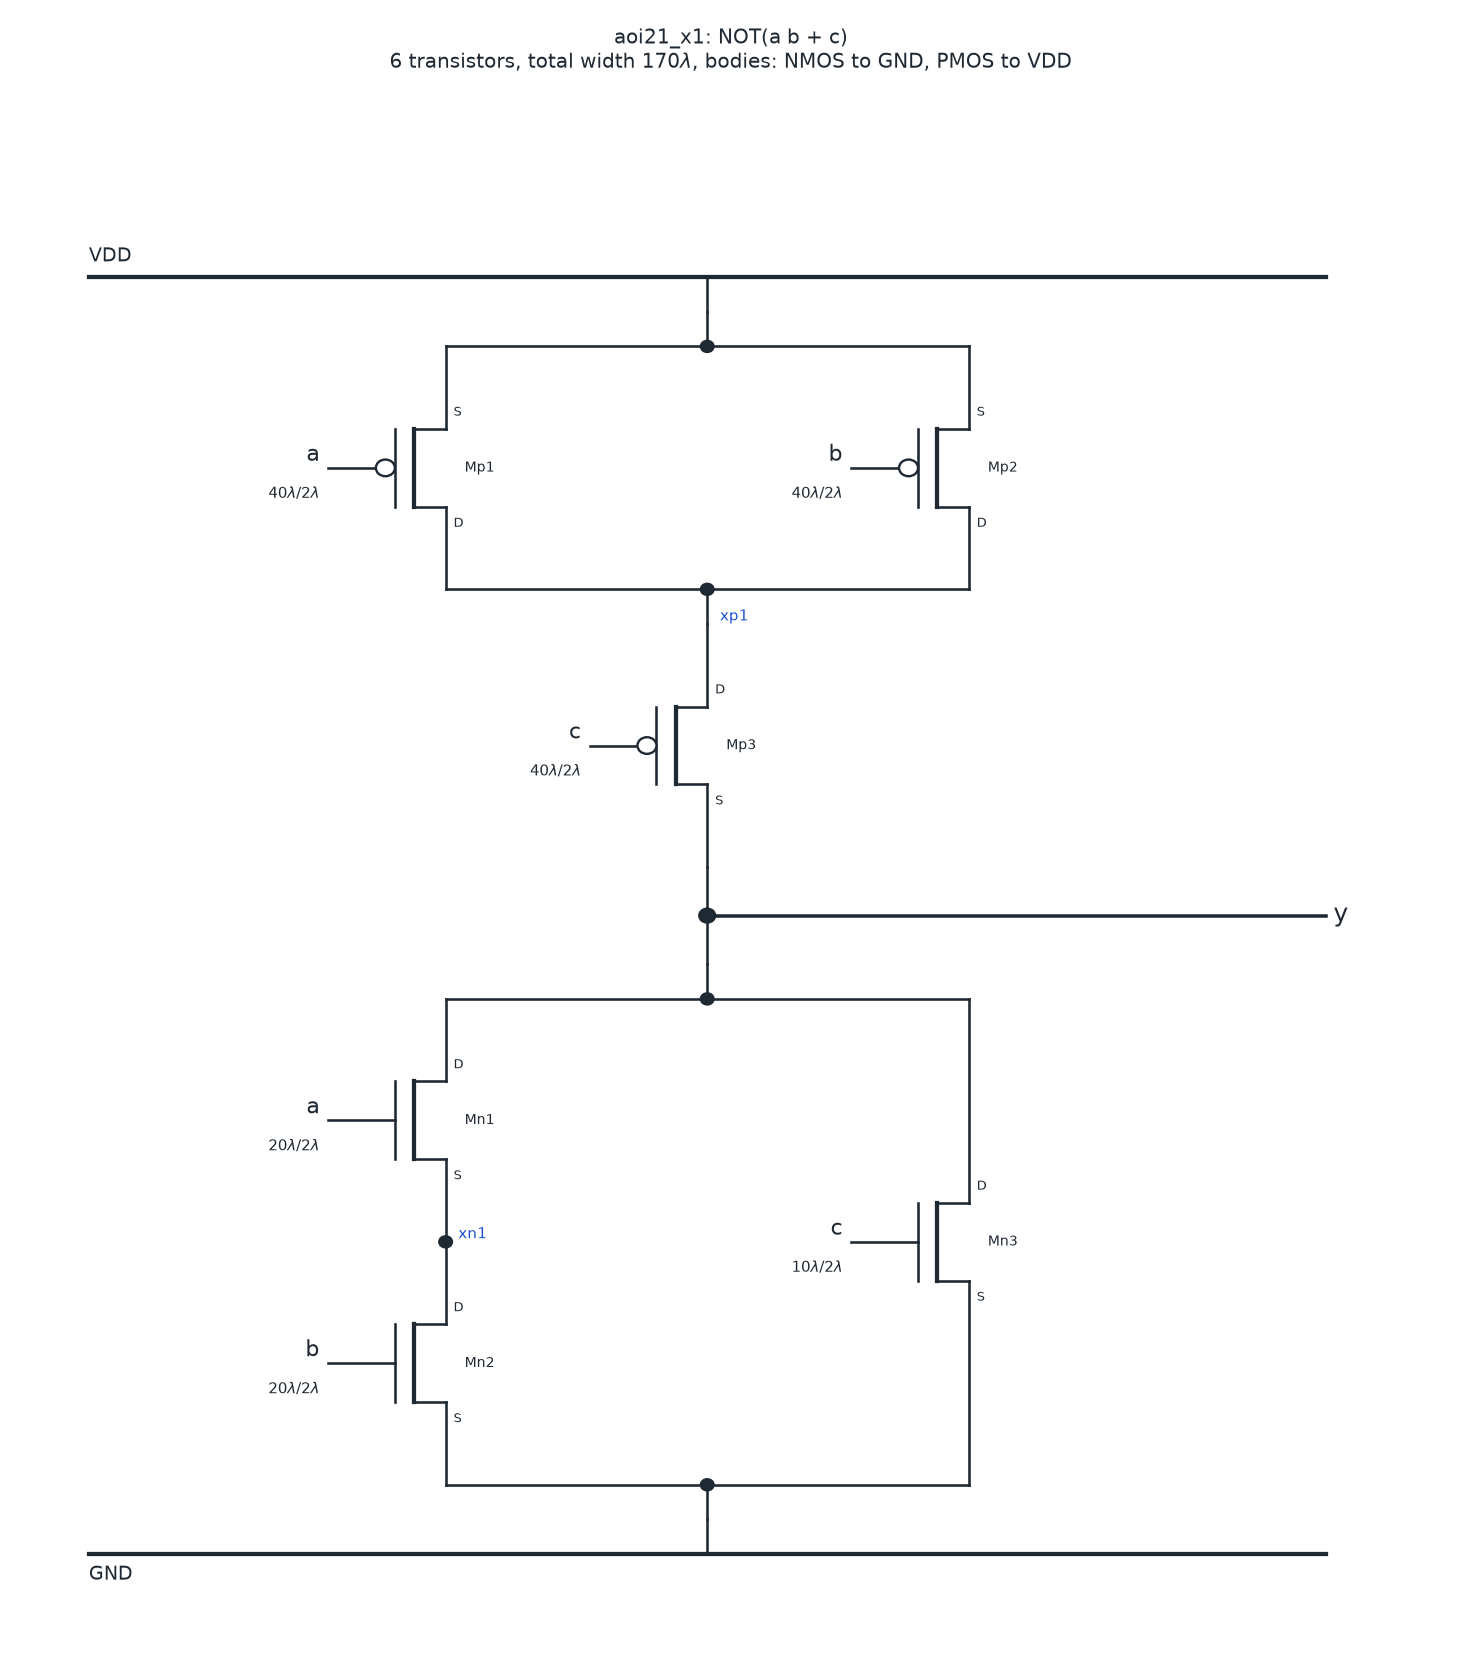
\includegraphics[width=0.8\columnwidth]{figures/final_aoi21_x1.png}\caption{Transistor schematic: AOI21, used for $p_i$ and the group generates.}\end{figure}

\begin{figure}[H]\centering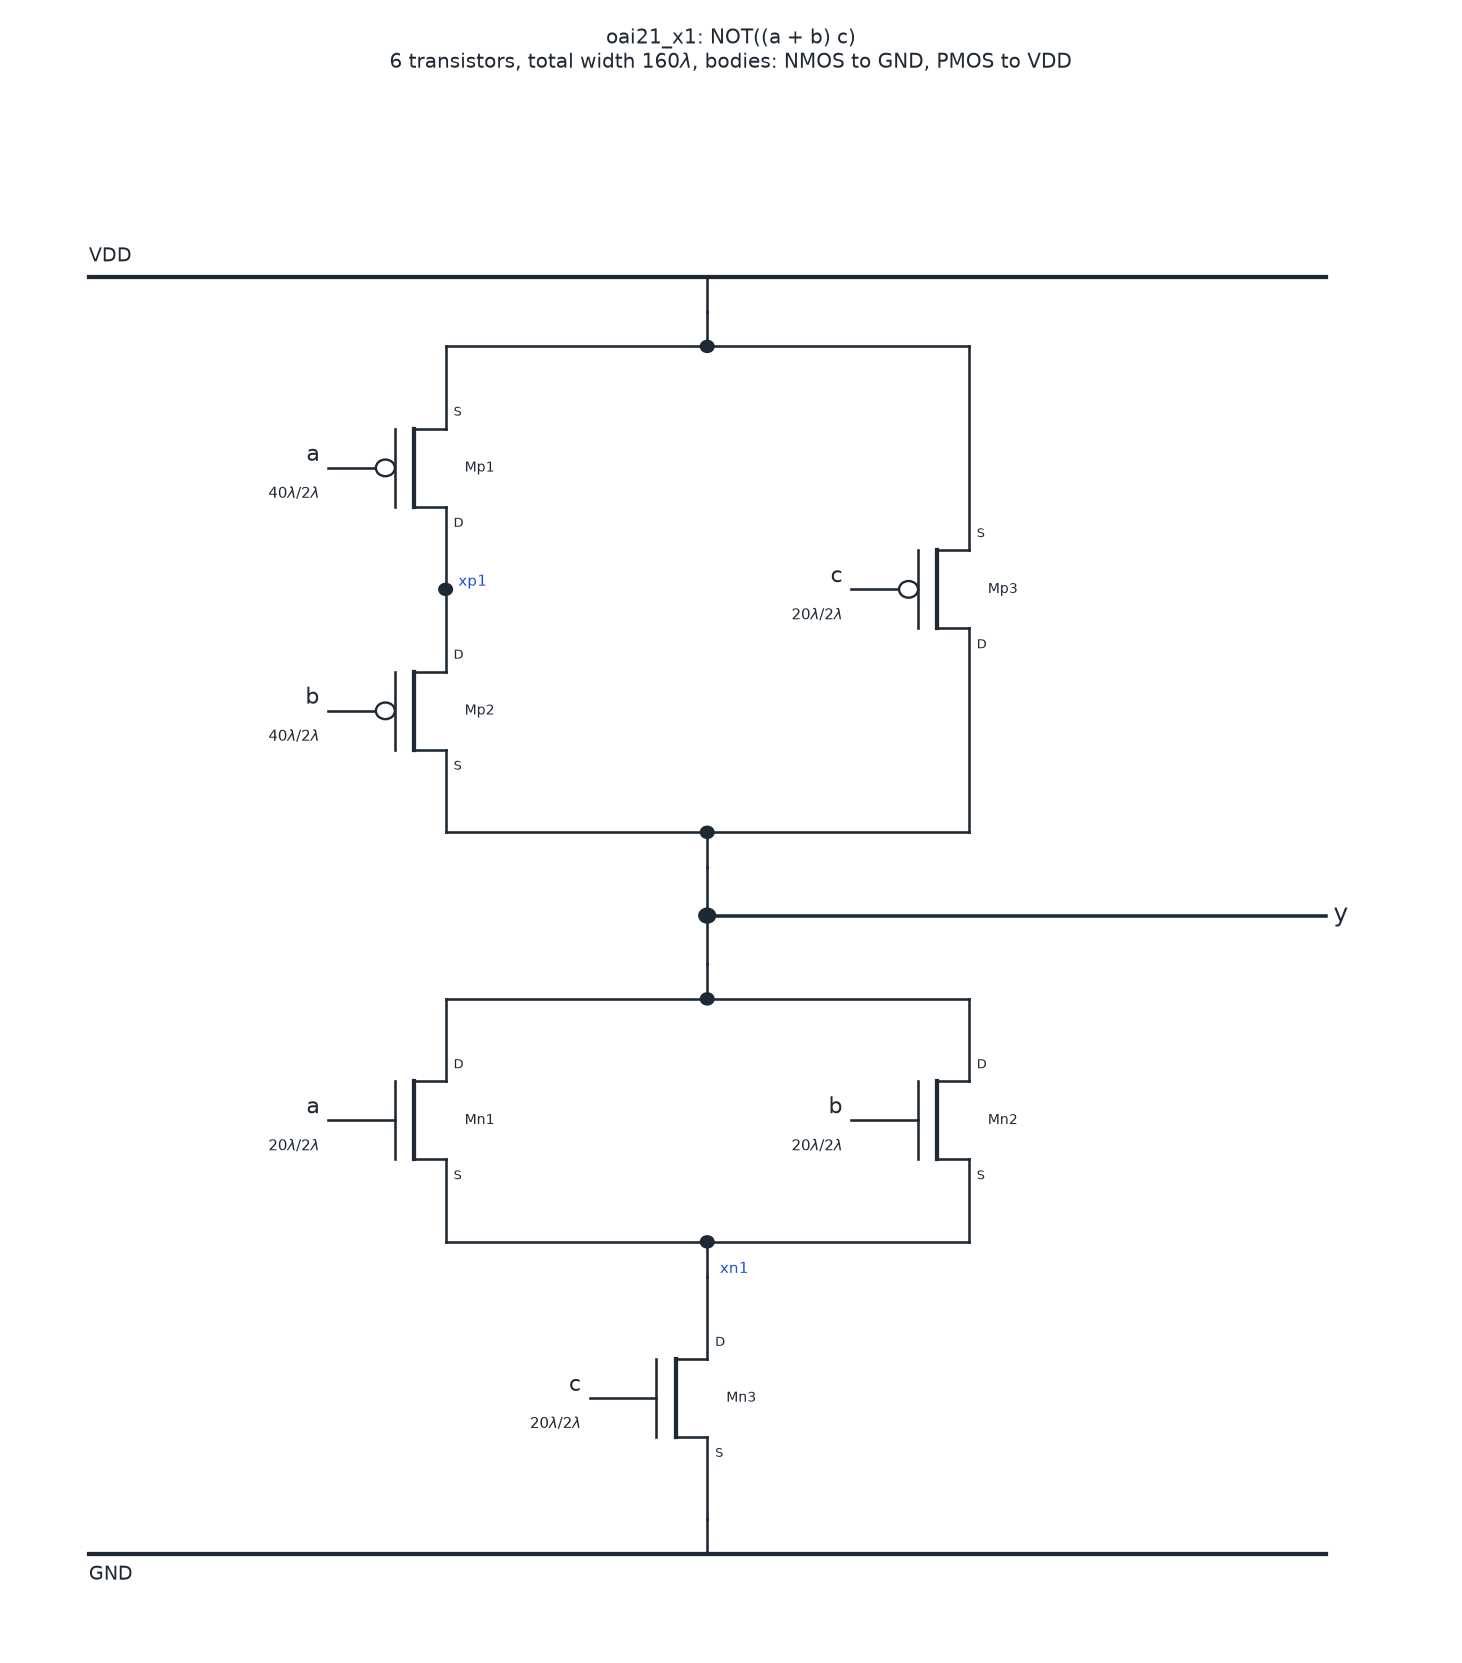
\includegraphics[width=0.8\columnwidth]{figures/final_oai21_x1.png}\caption{Transistor schematic: OAI21, used for $\overline{p_i}$ and the final carries.}\end{figure}

\subsection{Full Transistor-Level Schematic}
Figs.~\ref{fig:tl1}--\ref{fig:tl3} draw the whole adder transistor by transistor, all 194 devices with their final W/L. They are drawn from the final SPICE netlist, and every netlist transistor appears exactly once. The circuit is split by signal flow: the P/G front end, the prefix tree, then the final carries and sums. Gates connect by net name, so a net such as $\overline{\mathrm{G}}_{3:0}$ can be followed from the gate that drives it to every gate it feeds. The flip-flop used on all 14 inputs and outputs is in Fig.~\ref{fig:dffsch}. The figures are vector graphics and can be zoomed in the PDF.

\begin{figure*}[p]\centering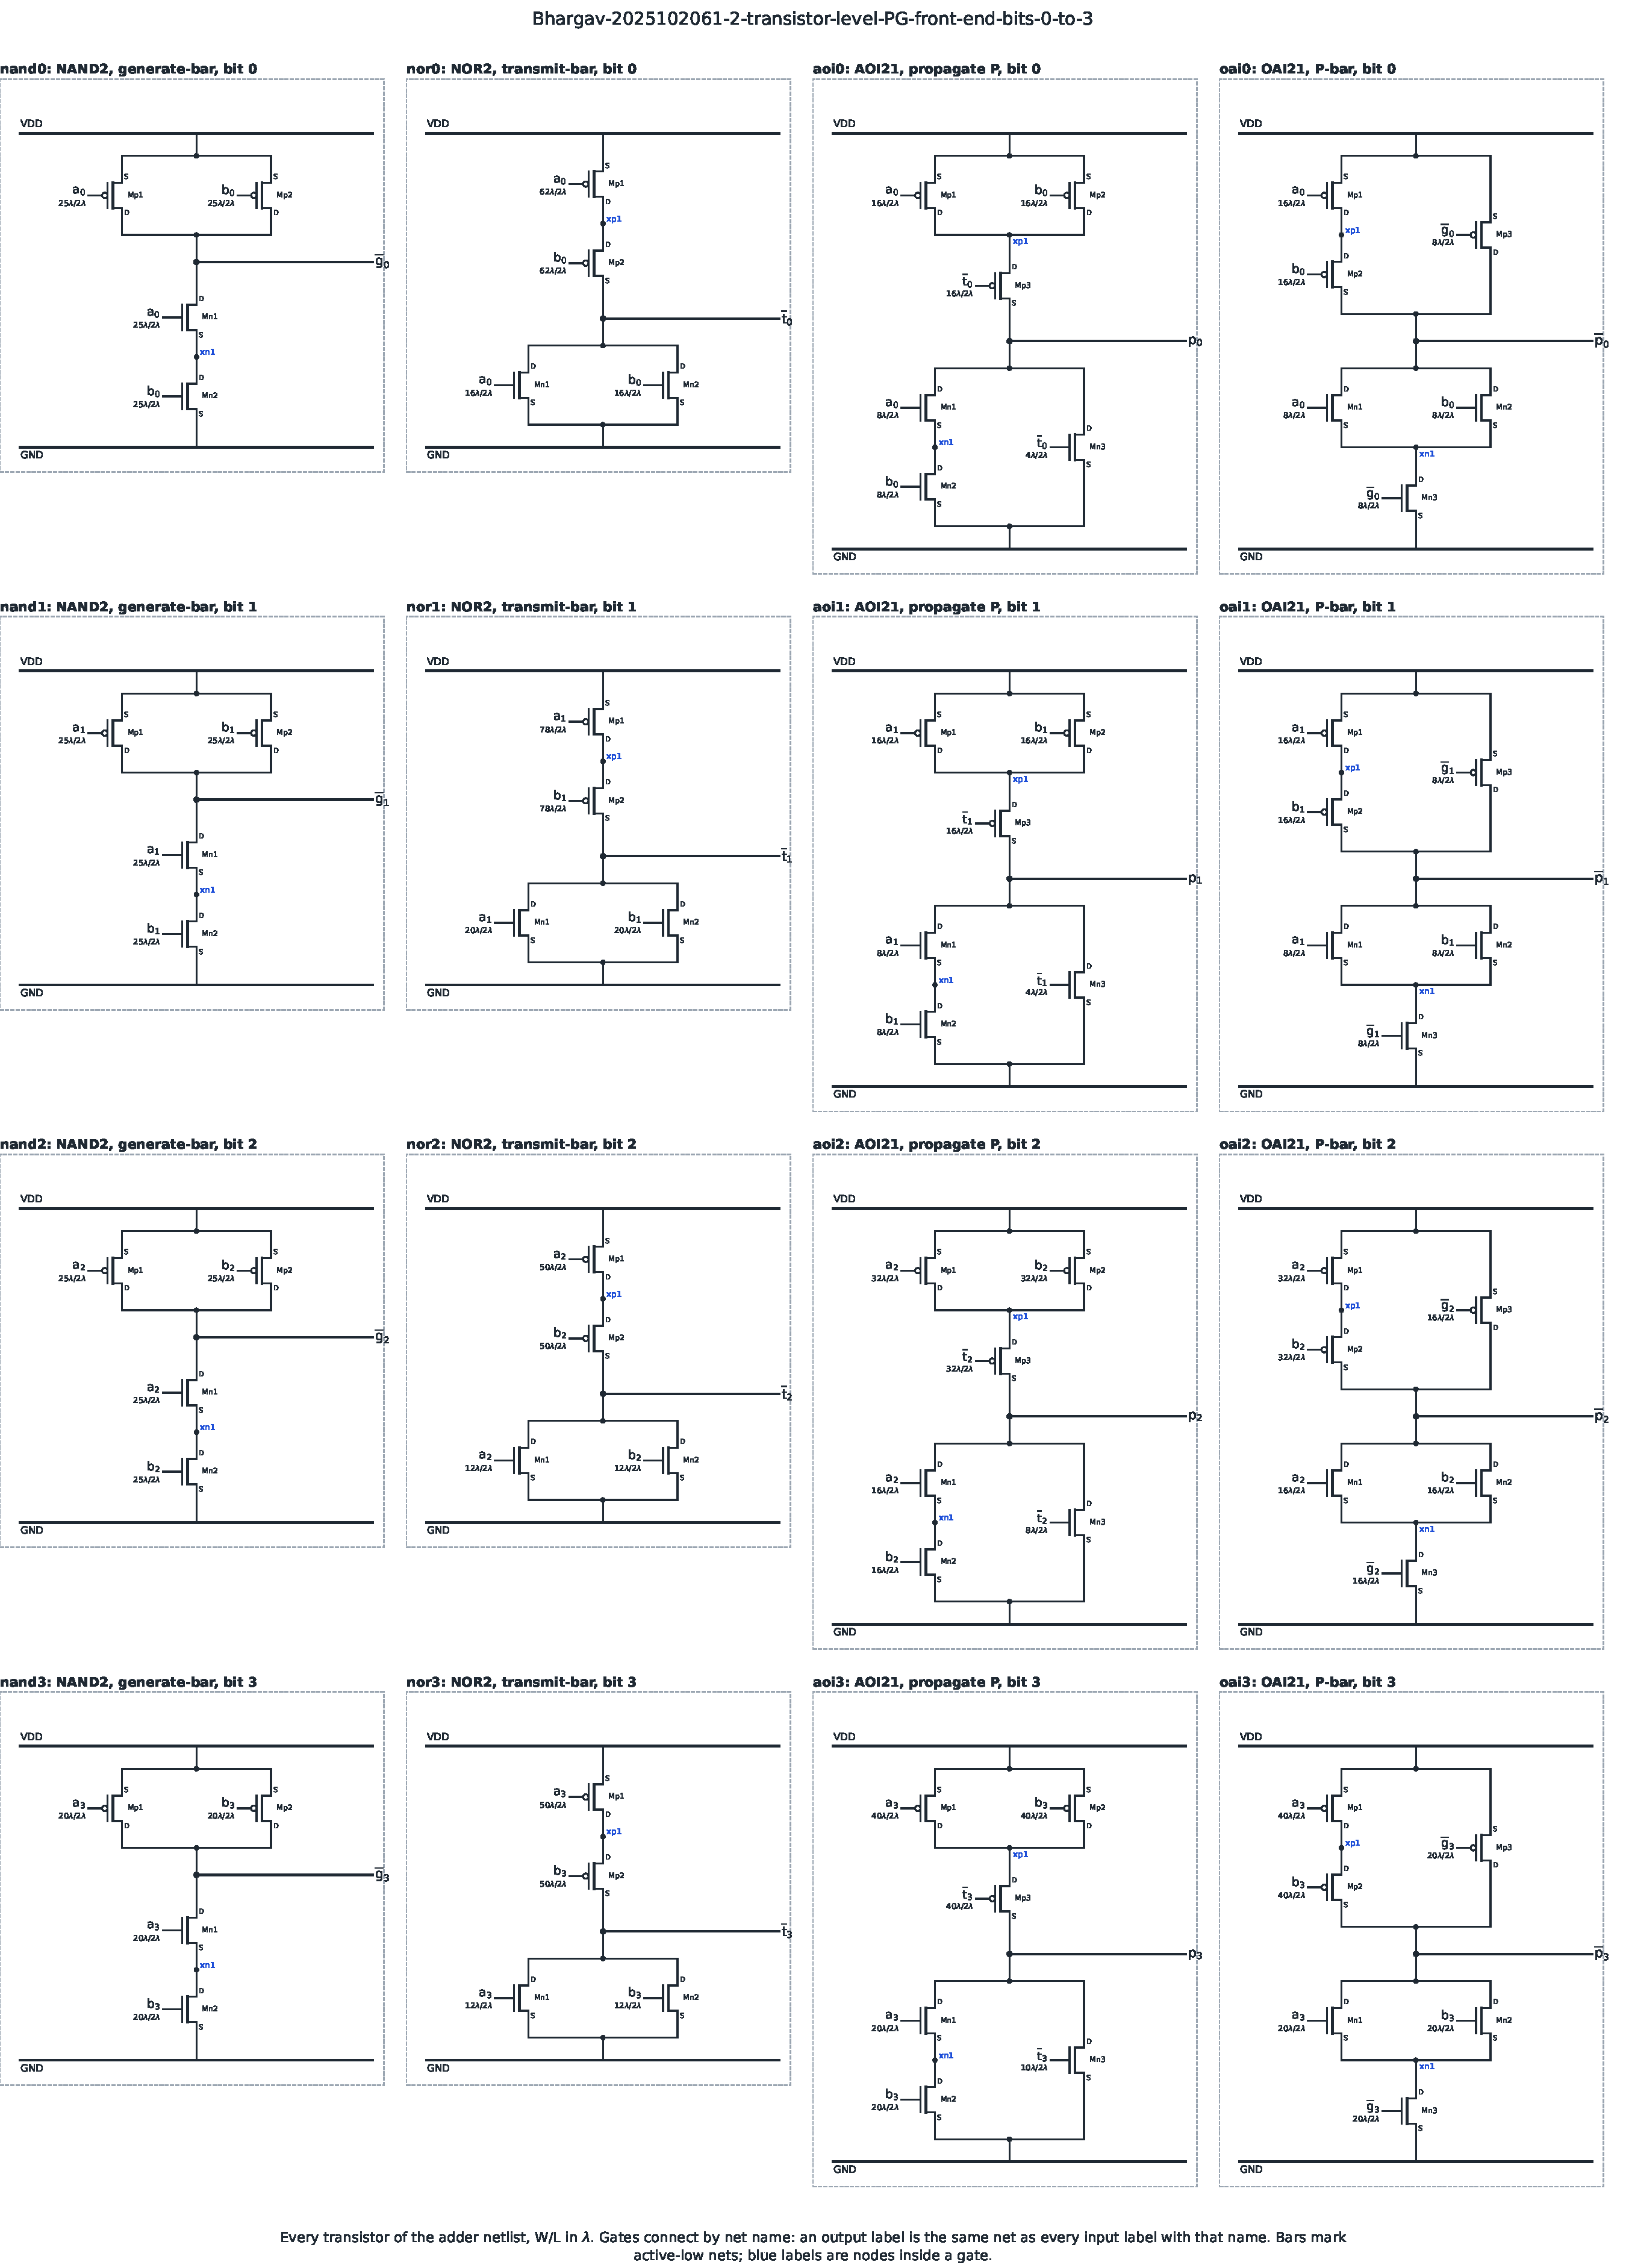
\includegraphics[width=\textwidth,height=0.9\textheight,keepaspectratio]{figures/full_tl_1_pg.pdf}\caption{Full adder, transistor level, part 1 of 3: P/G front end, bits 0 to 3 (80 transistors).}\label{fig:tl1}\end{figure*}

\begin{figure*}[p]\centering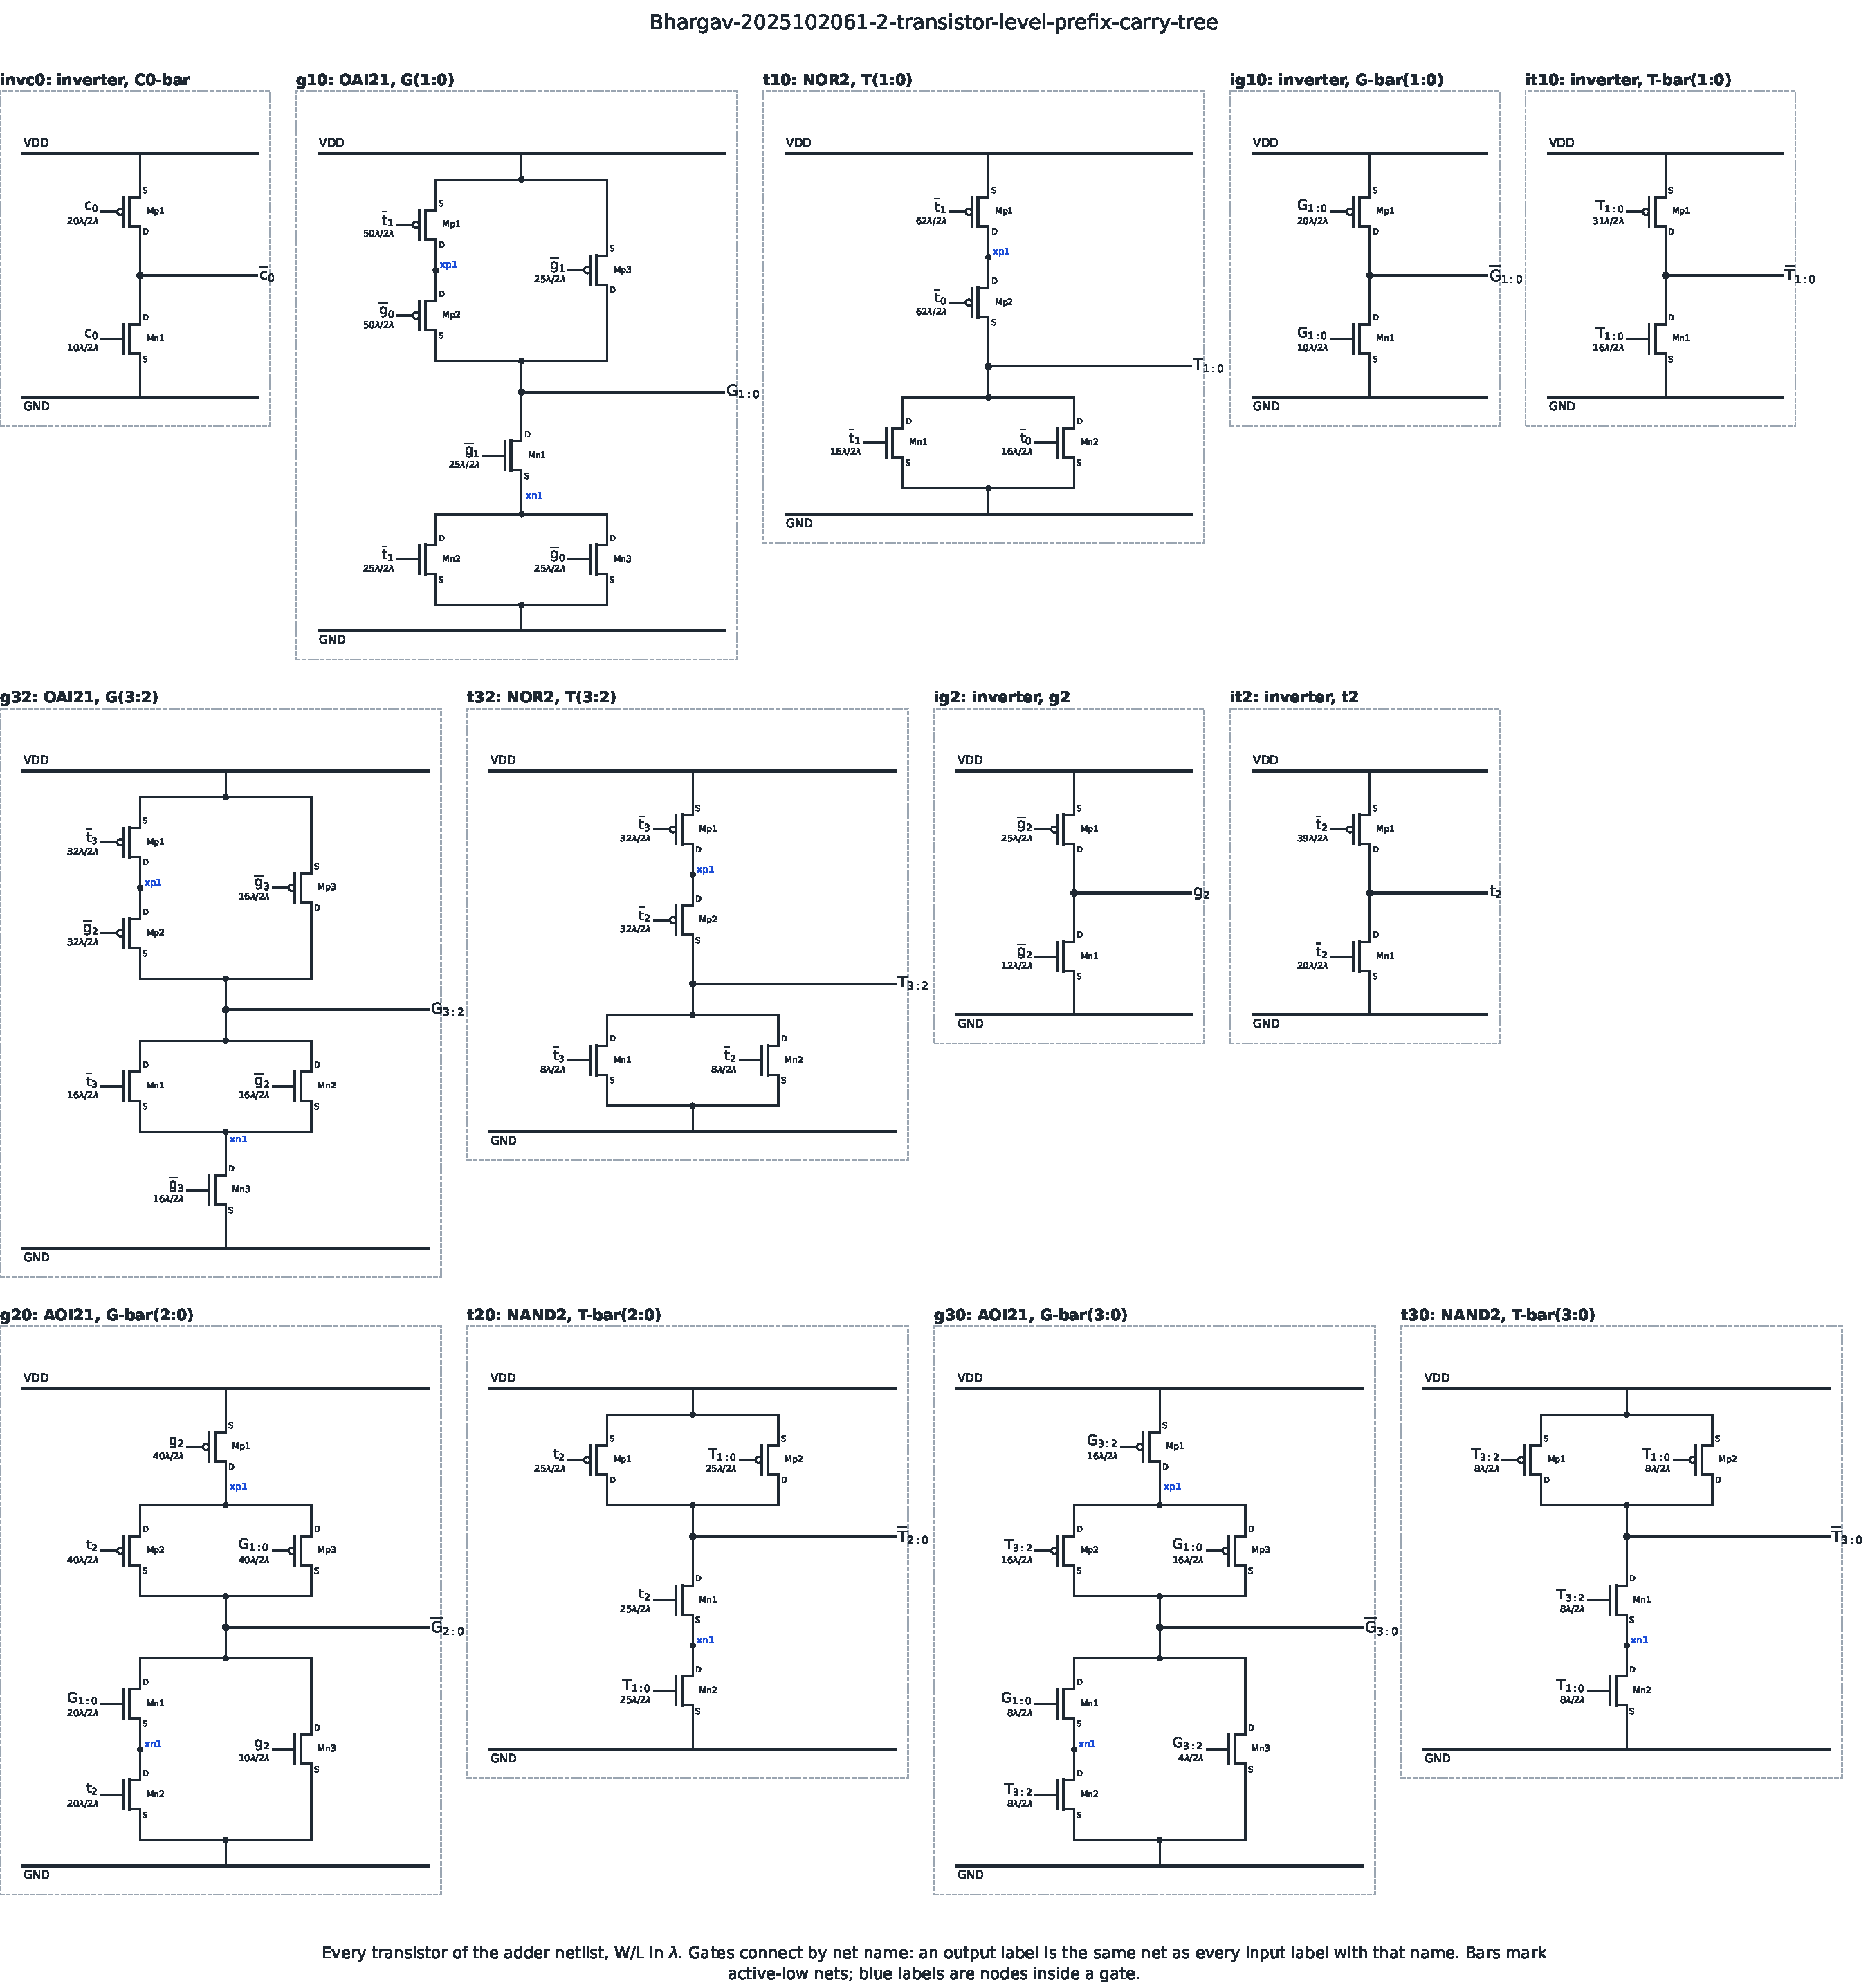
\includegraphics[width=\textwidth,height=0.9\textheight,keepaspectratio]{figures/full_tl_2_tree.pdf}\caption{Full adder, transistor level, part 2 of 3: prefix carry tree (50 transistors).}\label{fig:tl2}\end{figure*}

\begin{figure*}[p]\centering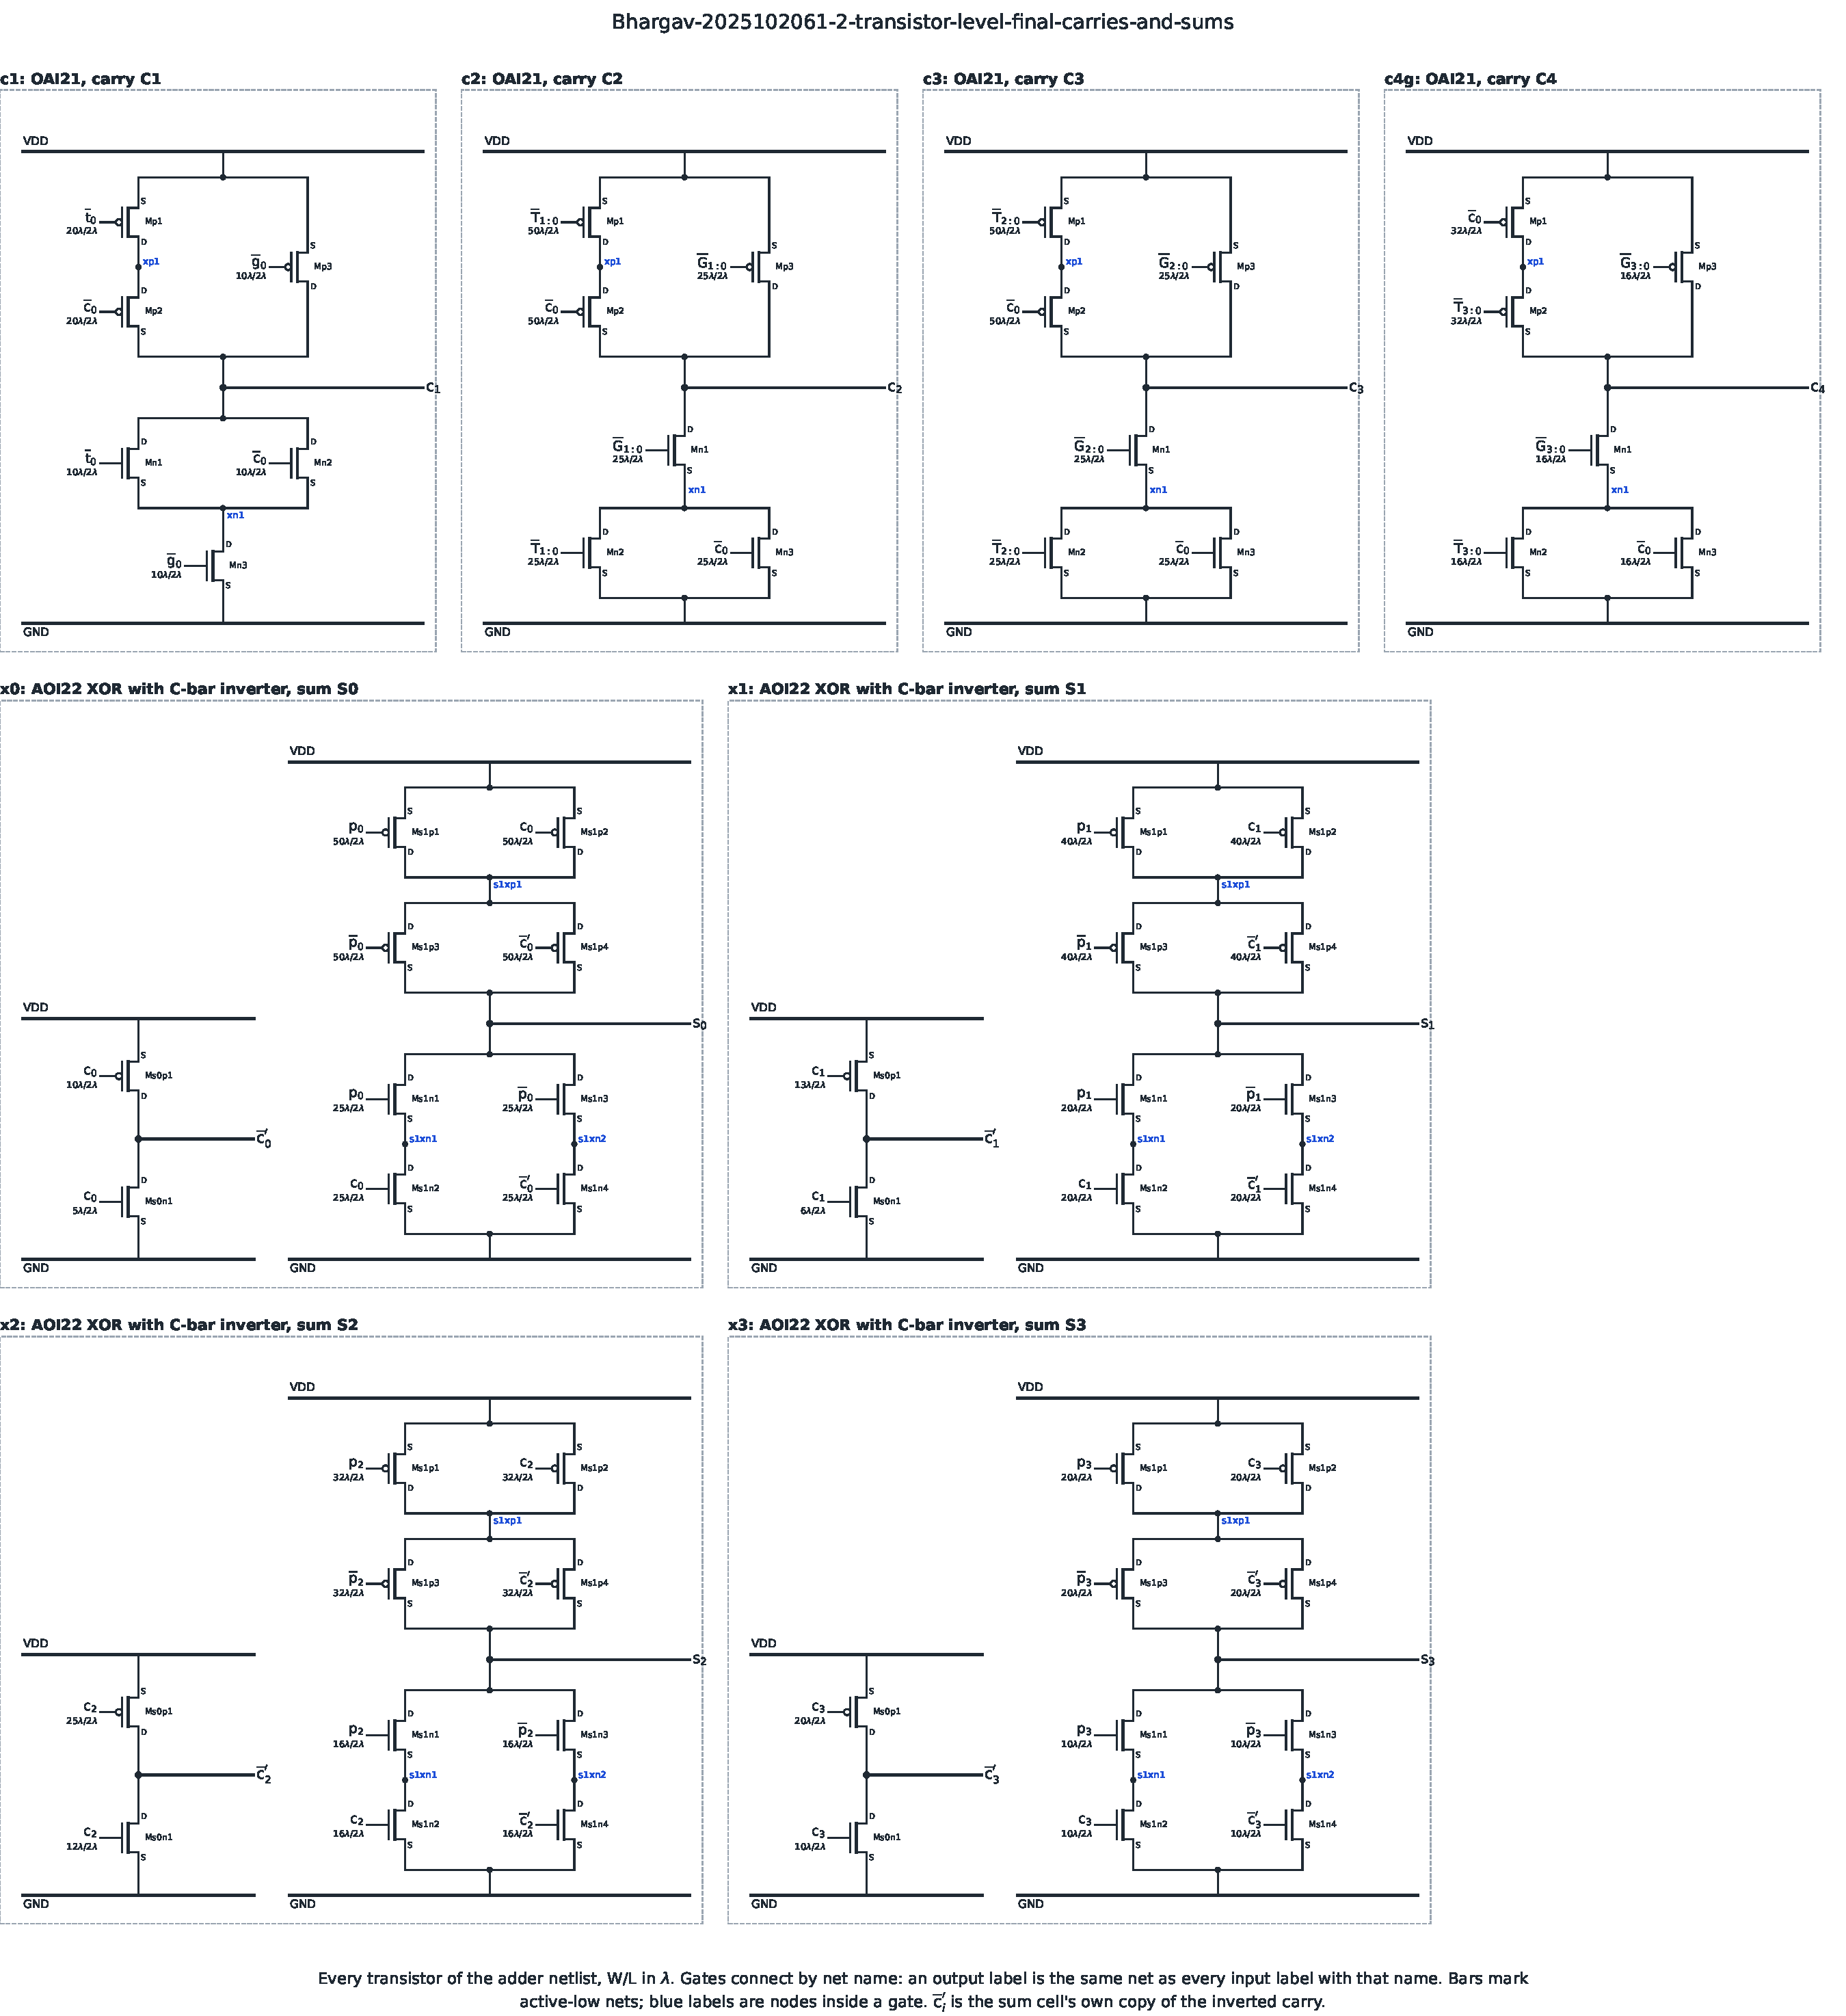
\includegraphics[width=\textwidth,height=0.9\textheight,keepaspectratio]{figures/full_tl_3_carry_sum.pdf}\caption{Full adder, transistor level, part 3 of 3: final carries $c_1$ to $c_4$ and the four sum cells (64 transistors).}\label{fig:tl3}\end{figure*}

\section{NGSPICE Simulation (Pre-Layout)}
Each gate is driven through two inverters, so its inputs have realistic edges, and its output drives the $20\lambda/10\lambda$ inverter. Inputs follow an Eulerian walk, which applies every single-input change from every state. Delay is measured from the 50\% point of the changing input to the last 50\% crossing of the output.

\subsection{Inverter}

\begin{figure}[H]\centering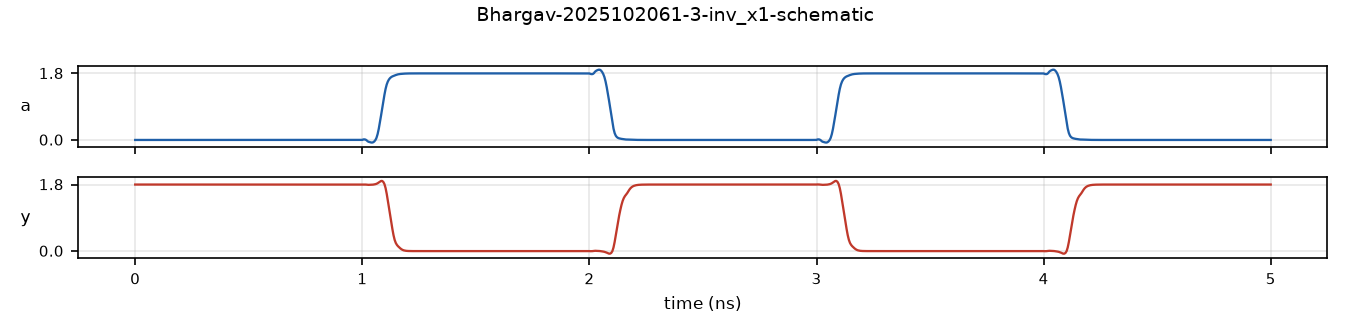
\includegraphics[width=\columnwidth]{figures/gate_inv_x1_schematic.png}\caption{Inverter plot: pre-layout.}\end{figure}

\subsection{NAND2}

\begin{figure}[H]\centering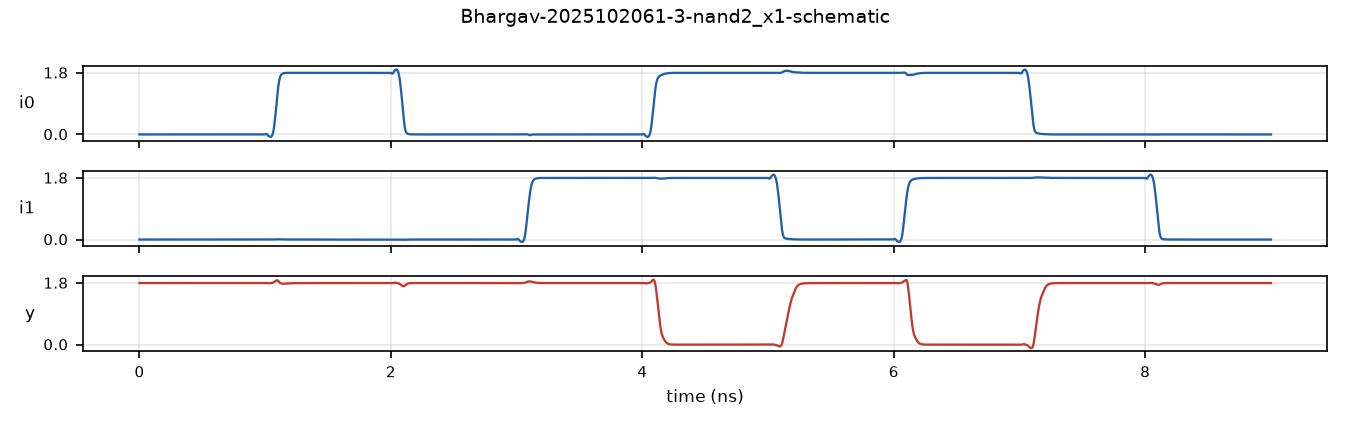
\includegraphics[width=\columnwidth]{figures/gate_nand2_x1_schematic.png}\caption{NAND2 plot: pre-layout.}\end{figure}

\subsection{NOR2}

\begin{figure}[H]\centering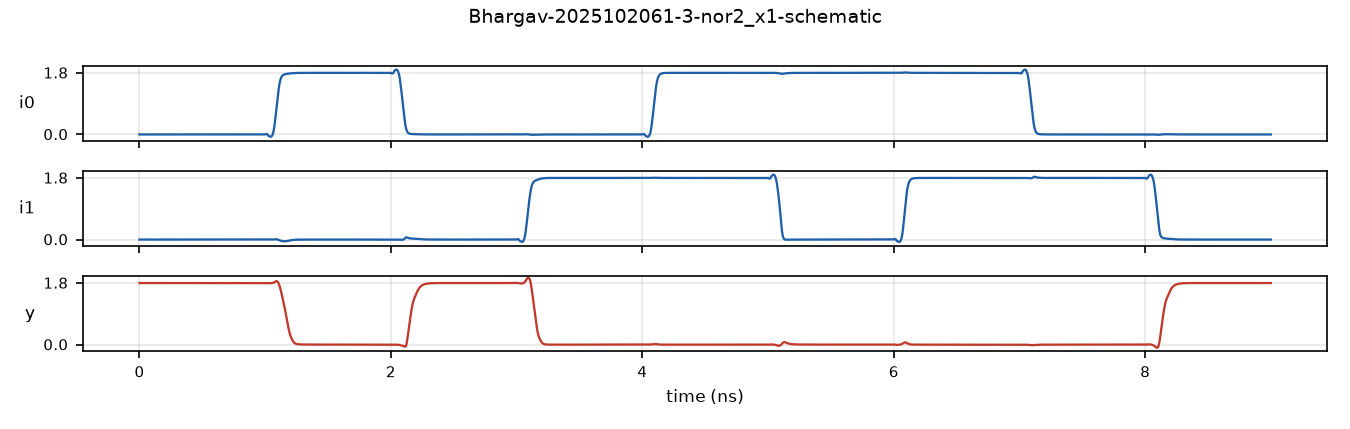
\includegraphics[width=\columnwidth]{figures/gate_nor2_x1_schematic.png}\caption{NOR2 plot: pre-layout.}\end{figure}

\subsection{AOI21}

\begin{figure}[H]\centering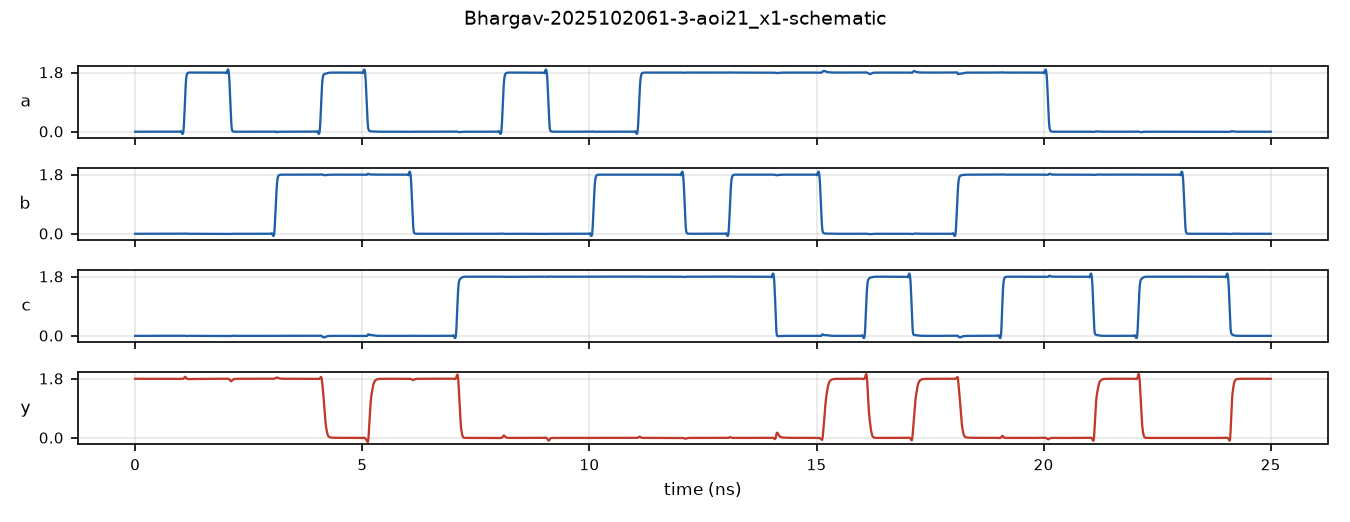
\includegraphics[width=\columnwidth]{figures/gate_aoi21_x1_schematic.png}\caption{AOI21 plot: pre-layout.}\end{figure}

\subsection{OAI21}

\begin{figure}[H]\centering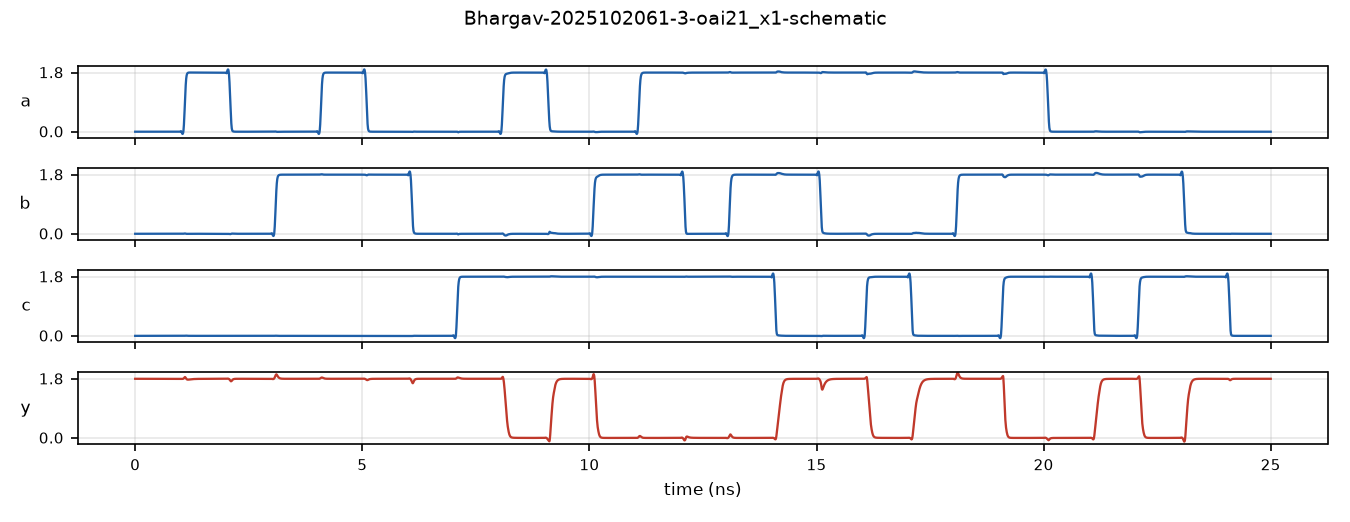
\includegraphics[width=\columnwidth]{figures/gate_oai21_x1_schematic.png}\caption{OAI21 plot: pre-layout.}\end{figure}

\subsection{AOI22 XOR (sum)}

\begin{figure}[H]\centering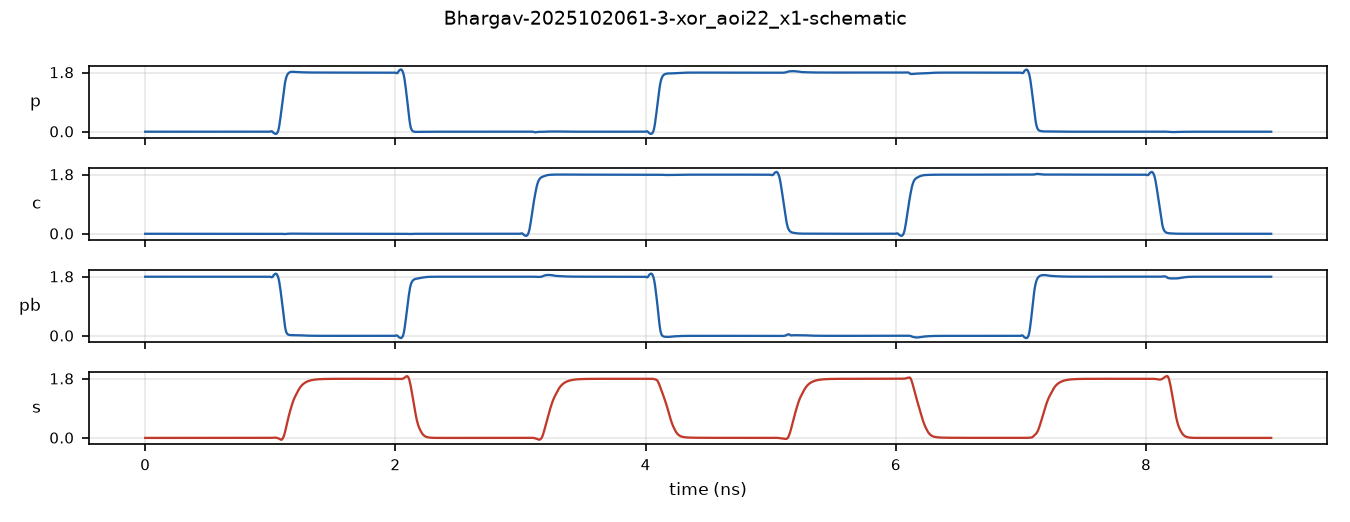
\includegraphics[width=\columnwidth]{figures/gate_xor_aoi22_x1_schematic.png}\caption{AOI22 XOR (sum) plot: pre-layout.}\end{figure}

\subsection{D Flip-Flop}

\begin{figure}[H]\centering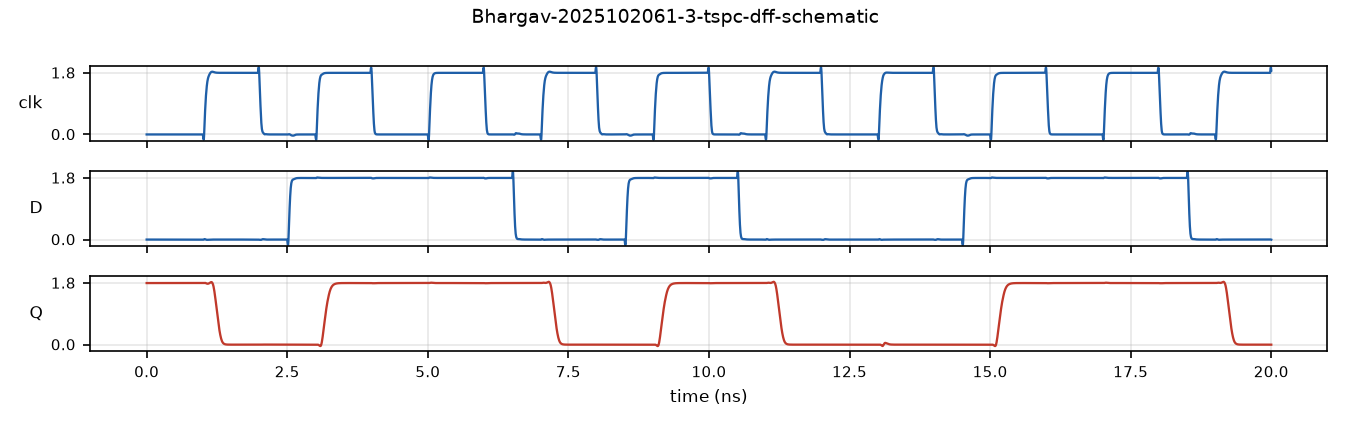
\includegraphics[width=\columnwidth]{figures/dff_schematic.png}\caption{TSPC D flip-flop plot: pre-layout. Q takes D at each rising clock edge.}\end{figure}

\subsection{P/G Block}

\begin{figure}[H]\centering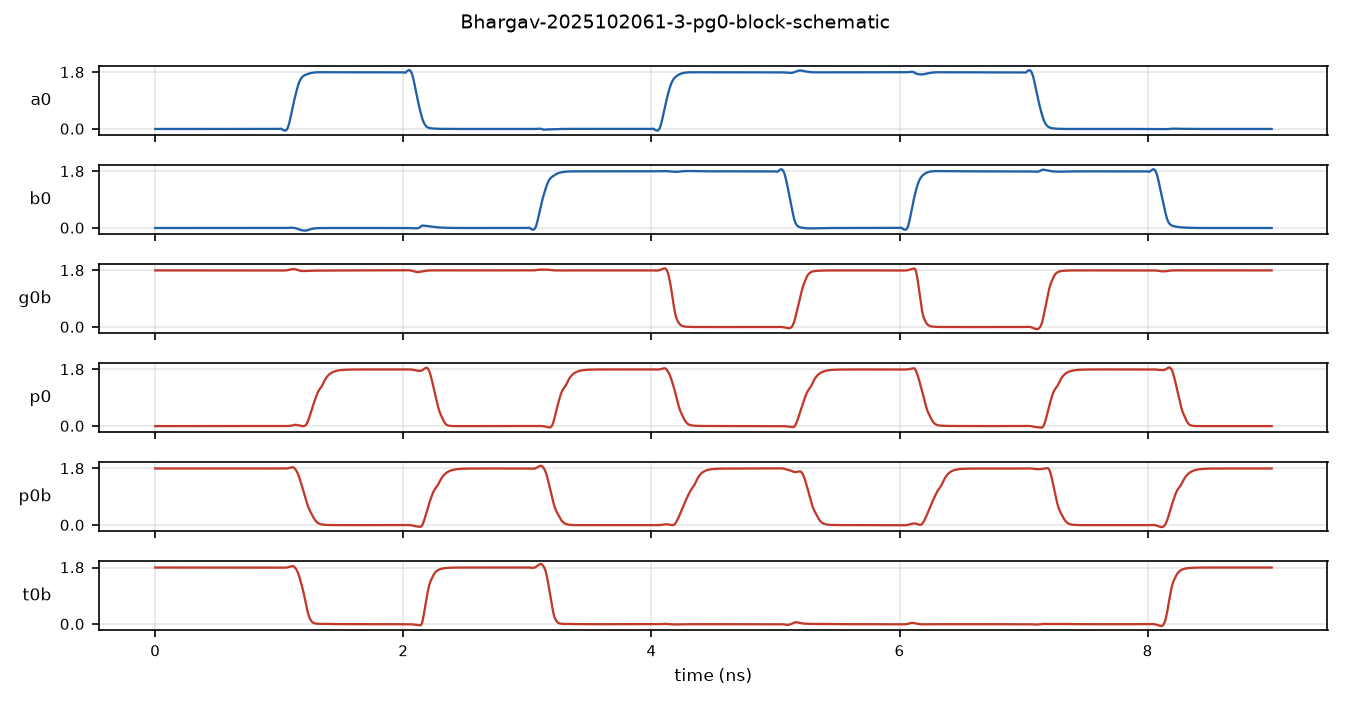
\includegraphics[width=\columnwidth]{figures/block_pg0_schematic.png}\caption{P/G Block plot: pre-layout.}\end{figure}

\subsection{Carry Block}

\begin{figure}[H]\centering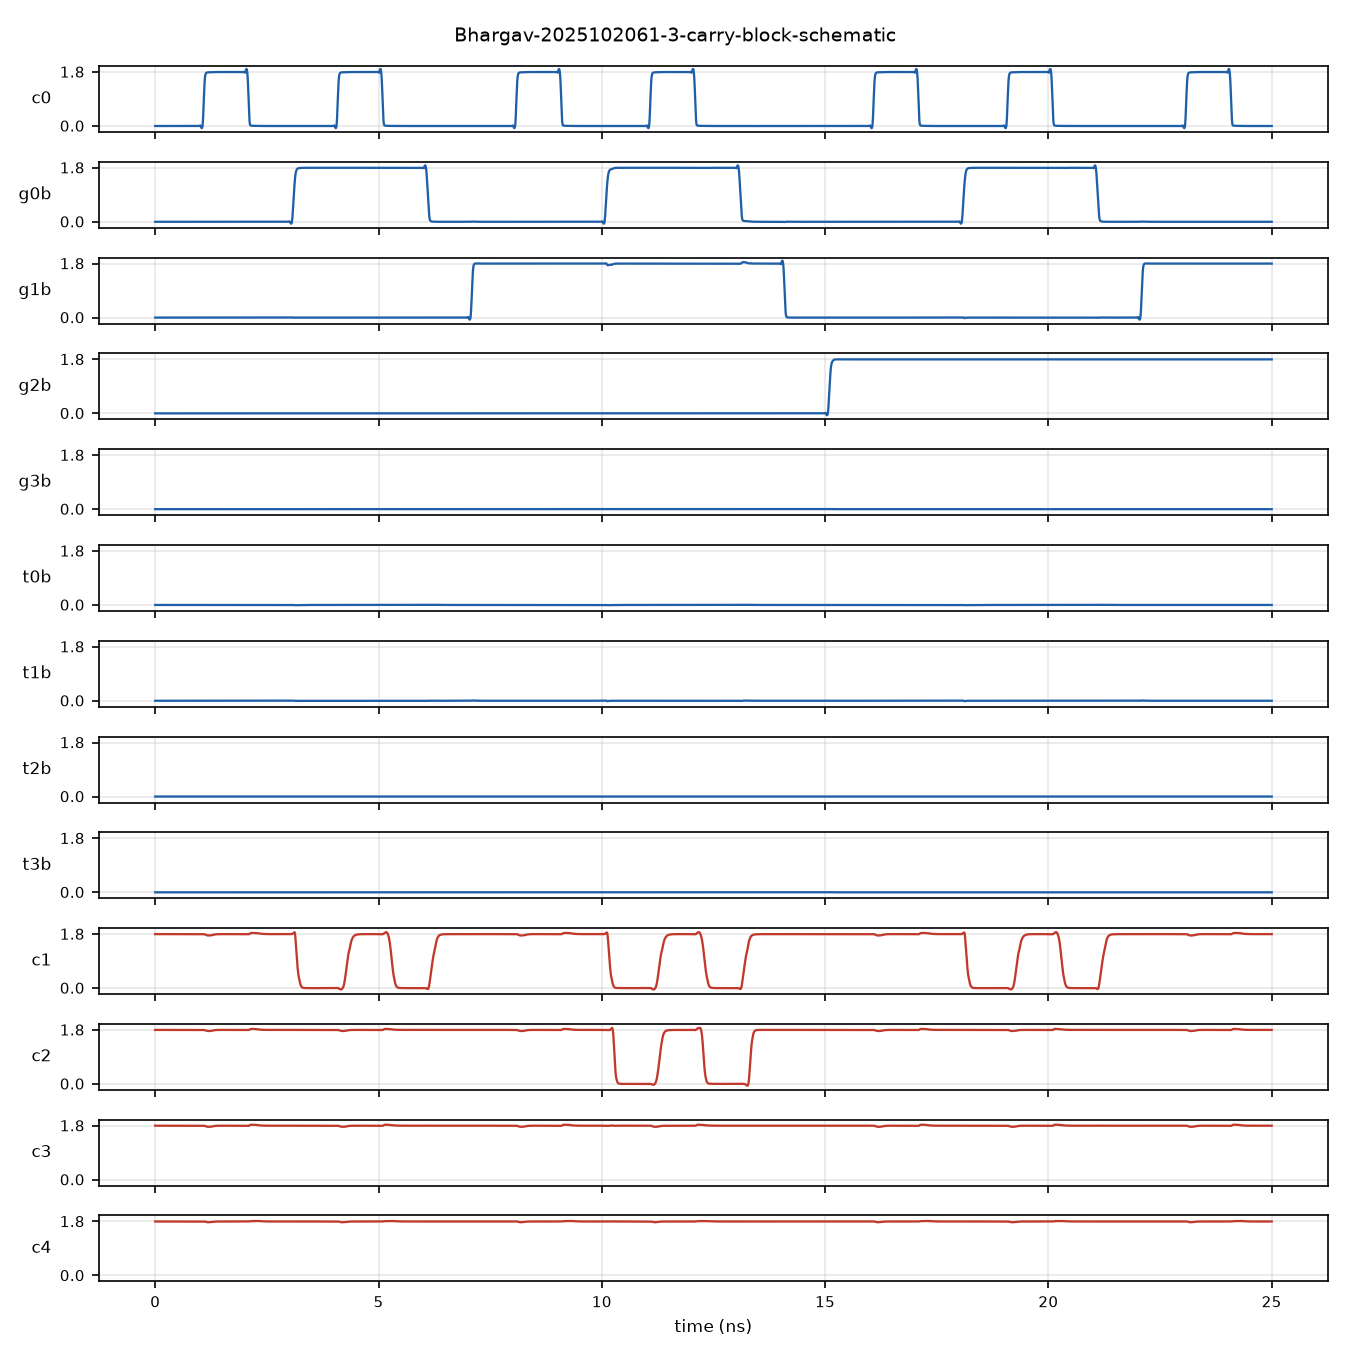
\includegraphics[width=\columnwidth]{figures/block_carry_schematic.png}\caption{Carry Block plot: pre-layout.}\end{figure}

\subsection{Sum Block}

\begin{figure}[H]\centering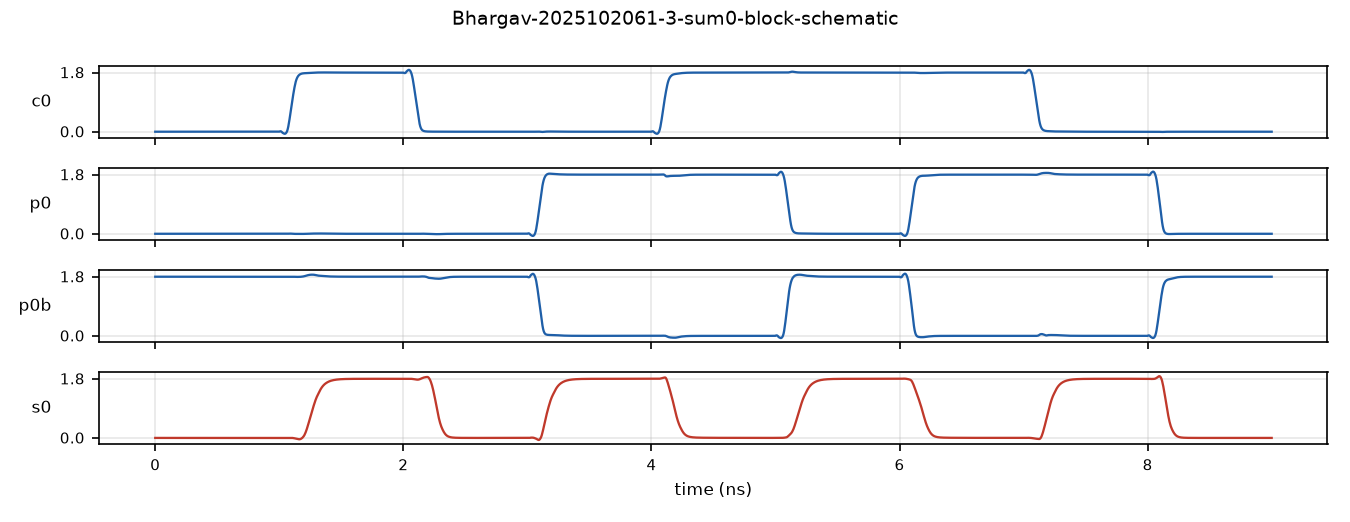
\includegraphics[width=\columnwidth]{figures/block_sum0_schematic.png}\caption{Sum Block plot: pre-layout.}\end{figure}

\begin{table}[H]\centering\footnotesize
\caption{Gate delays, pre-layout, worst over all single-input changes}
\begin{tabular}{|c|c|c|c|}\hline
Gate & tpLH (ps) & tpHL (ps) & Errors \\ \hline
Inverter & 38.59 & 35.7 & 0 \\ \hline
NAND2 & 66.02 & 45.44 & 0 \\ \hline
NOR2 & 64.35 & 70.61 & 0 \\ \hline
AOI21 & 91.52 & 74.76 & 0 \\ \hline
OAI21 & 92.91 & 75.84 & 0 \\ \hline
AOI22 XOR (sum) & 134.99 & 122.89 & 0 \\ \hline
\end{tabular}
\end{table}

\section{D Flip-Flop Characterization from NGSPICE}
\subsection{TSPC Flip-Flop}
The flip-flop is characterised at its real load, 47.76\,fF, with both data values. Definitions follow Stojanovi\'c and Oklobd\v{z}ija~\cite{stoj}.
\subsection{Clock to Q Delay $t_{cq}$}
Time from the 50\% point of the rising clock to the 50\% point of Q, with data set up long before the edge.

\begin{table}[H]\centering\footnotesize
\caption{Clock to Q delay, pre-layout}
\begin{tabular}{|c|c|}\hline
Parameter & Time (ps) \\ \hline
$t_{cq}$, Q rising & 134.1 \\ \hline
$t_{cq}$, Q falling & 208.5 \\ \hline
$t_{cq}$ (worst) & 208.5 \\ \hline
\end{tabular}
\end{table}

\subsection{Set Up Time $t_{su}$}
The shortest D-to-clock time for which clock-to-Q stays within 10\% of its long-setup value.

\begin{table}[H]\centering\footnotesize
\caption{Set up time, pre-layout}
\begin{tabular}{|c|c|}\hline
Parameter & Time (ps) \\ \hline
$t_{su}$, D rising & -26.0 \\ \hline
$t_{su}$, D falling & 34.0 \\ \hline
$t_{su}$ (worst) & 34.0 \\ \hline
\end{tabular}
\end{table}

\subsection{Hold Time $t_{hold}$}
The shortest clock-to-D time for which a later data change leaves Q correct, with no disturbance above 10\% of $V_{DD}$.

\begin{table}[H]\centering\footnotesize
\caption{Hold time, pre-layout}
\begin{tabular}{|c|c|}\hline
Parameter & Time (ps) \\ \hline
$t_{hold}$, D rising & -11.7 \\ \hline
$t_{hold}$, D falling & 55.1 \\ \hline
$t_{hold}$ (worst) & 55.1 \\ \hline
\end{tabular}
\end{table}

\begin{figure}[H]\centering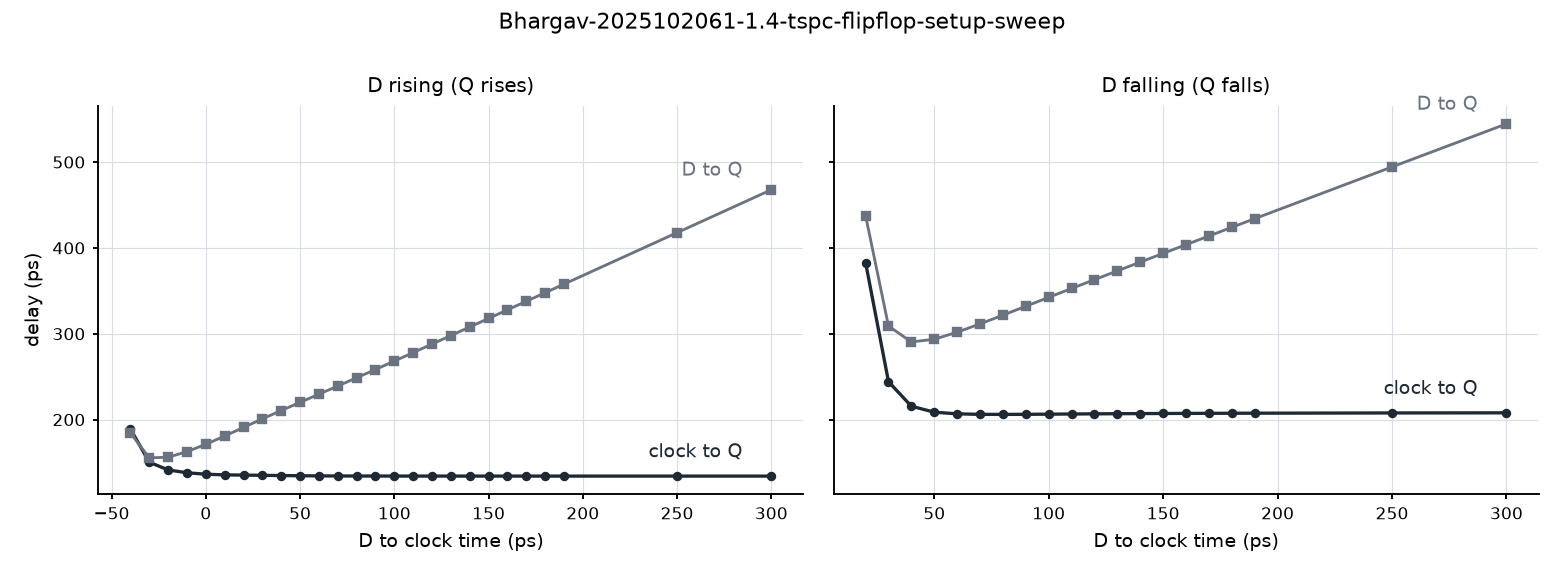
\includegraphics[width=\columnwidth]{figures/figures_dff_sweep.png}\caption{Clock-to-Q and D-to-Q delay against D-to-clock time, schematic.}\end{figure}

\section{Euler Paths and Stick Diagrams}
Each gate is laid out as one PMOS row and one NMOS row of diffusion, crossed by vertical poly gates. Two neighbouring transistors in a row can share a diffusion node, with no gap and no extra contact, only if they connect to the same net there. A row with no breaks is therefore an Euler path through the network's graph: the nodes are the diffusion nets, and each edge is one transistor, labelled by its gate input. Using the same gate order in the PMOS and NMOS rows lets one straight poly line serve both transistors on the same input.

Each cell's layout follows the ordering shown in its figure. In the Euler graphs, the number on each edge is its position along the row. The stick diagrams are the MAGIC layouts with every rectangle reduced to its centre line: diffusion, poly and metal as coloured sticks, contacts as crosses. Each matches the layout in Section~\ref{sec:magic}, not a separate sketch.

\begin{table*}[!t]\centering\footnotesize
\caption{Gate order along the diffusion rows (from the MAGIC layouts)}
\begin{tabular}{|c|c|c|c|c|}\hline
Cell & PMOS row & NMOS row & Breaks P/N & Same order \\ \hline
Inverter & $\mathrm{a}$ & $\mathrm{a}$ & 0/0 & yes \\ \hline
NAND2 & $\mathrm{i}_{0}$ $\to$ $\mathrm{i}_{1}$ & $\mathrm{i}_{0}$ $\to$ $\mathrm{i}_{1}$ & 0/0 & yes \\ \hline
NOR2 & $\mathrm{i}_{0}$ $\to$ $\mathrm{i}_{1}$ & $\mathrm{i}_{0}$ $\to$ $\mathrm{i}_{1}$ & 0/0 & yes \\ \hline
AOI21 & $\mathrm{a}$ $\to$ $\mathrm{b}$ $\to$ $\mathrm{c}$ & $\mathrm{a}$ $\to$ $\mathrm{b}$ $\to$ $\mathrm{c}$ & 0/0 & yes \\ \hline
OAI21 & $\mathrm{a}$ $\to$ $\mathrm{b}$ $\to$ $\mathrm{c}$ & $\mathrm{a}$ $\to$ $\mathrm{b}$ $\to$ $\mathrm{c}$ & 0/0 & yes \\ \hline
AOI22 XOR & $\mathrm{c}$ $\to$ $\mathrm{p}$ $\to$ $\overline{\mathrm{p}}$ $\to$ $\overline{\mathrm{c}}$ $\to$ $\mathrm{c}$ & $\mathrm{c}$ $\to$ $\mathrm{p}$ $\to$ $\overline{\mathrm{p}}$ $\to$ $\overline{\mathrm{c}}$ $\to$ $\mathrm{c}$ & 0/0 & yes \\ \hline
TSPC flip-flop & $\mathrm{clk}$ $\to$ $\mathrm{d}$ $\to$ $\mathrm{b}$ $\to$ $\mathrm{clk}$ $\to$ $\overline{\mathrm{q}}$ & $\mathrm{a}$ $\to$ $\mathrm{clk}$ $\to$ $\mathrm{b}$ $\to$ $\mathrm{clk}$ $\to$ $\overline{\mathrm{q}}$ $\to$ $\mathrm{d}$ & 1/1 & no \\ \hline
\end{tabular}
\end{table*}

Every logic gate gets an unbroken Euler path in both rows with a common gate order, so each input is one poly line and no row needs a diffusion break. The AOI22 XOR shares its rows with the carry inverter, so input $c$ appears twice. The TSPC flip-flop has four stages with different inputs, and needs one break in each row. Where the PMOS and NMOS gates in a column differ, the poly is split into separate top and bottom gates.

\begin{figure*}[!t]\centering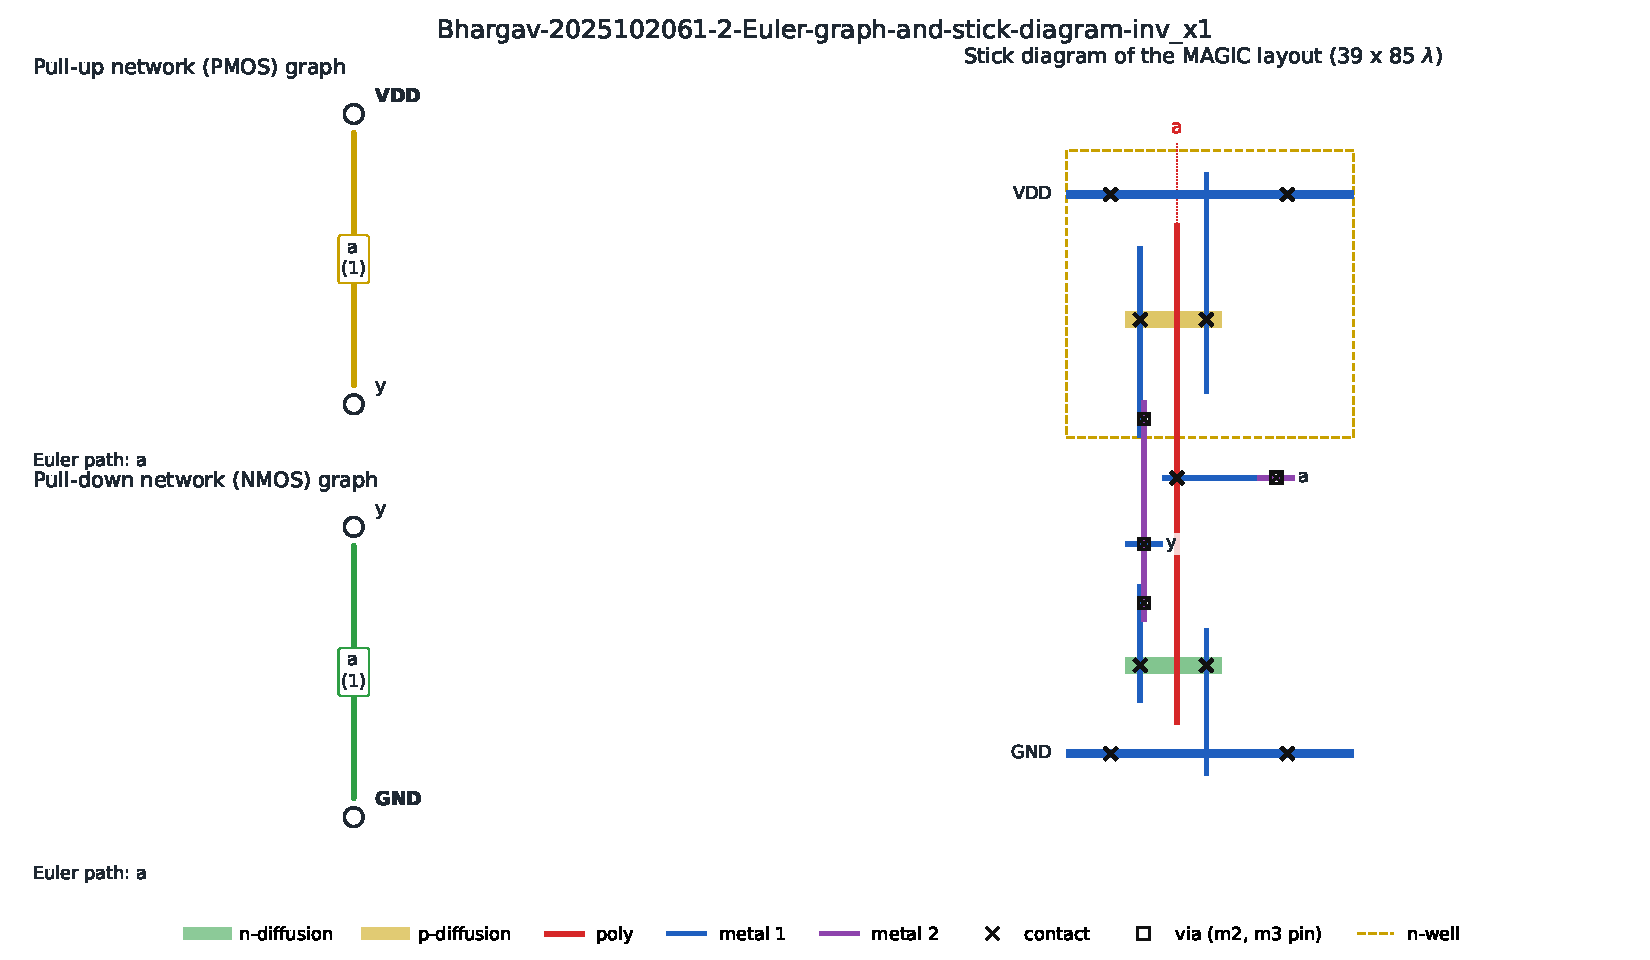
\includegraphics[width=\textwidth]{figures/stick_inv_x1.pdf}\caption{Euler graphs of the pull-up and pull-down networks, and stick diagram of the MAGIC layout: Inverter.}\end{figure*}

\begin{figure*}[!t]\centering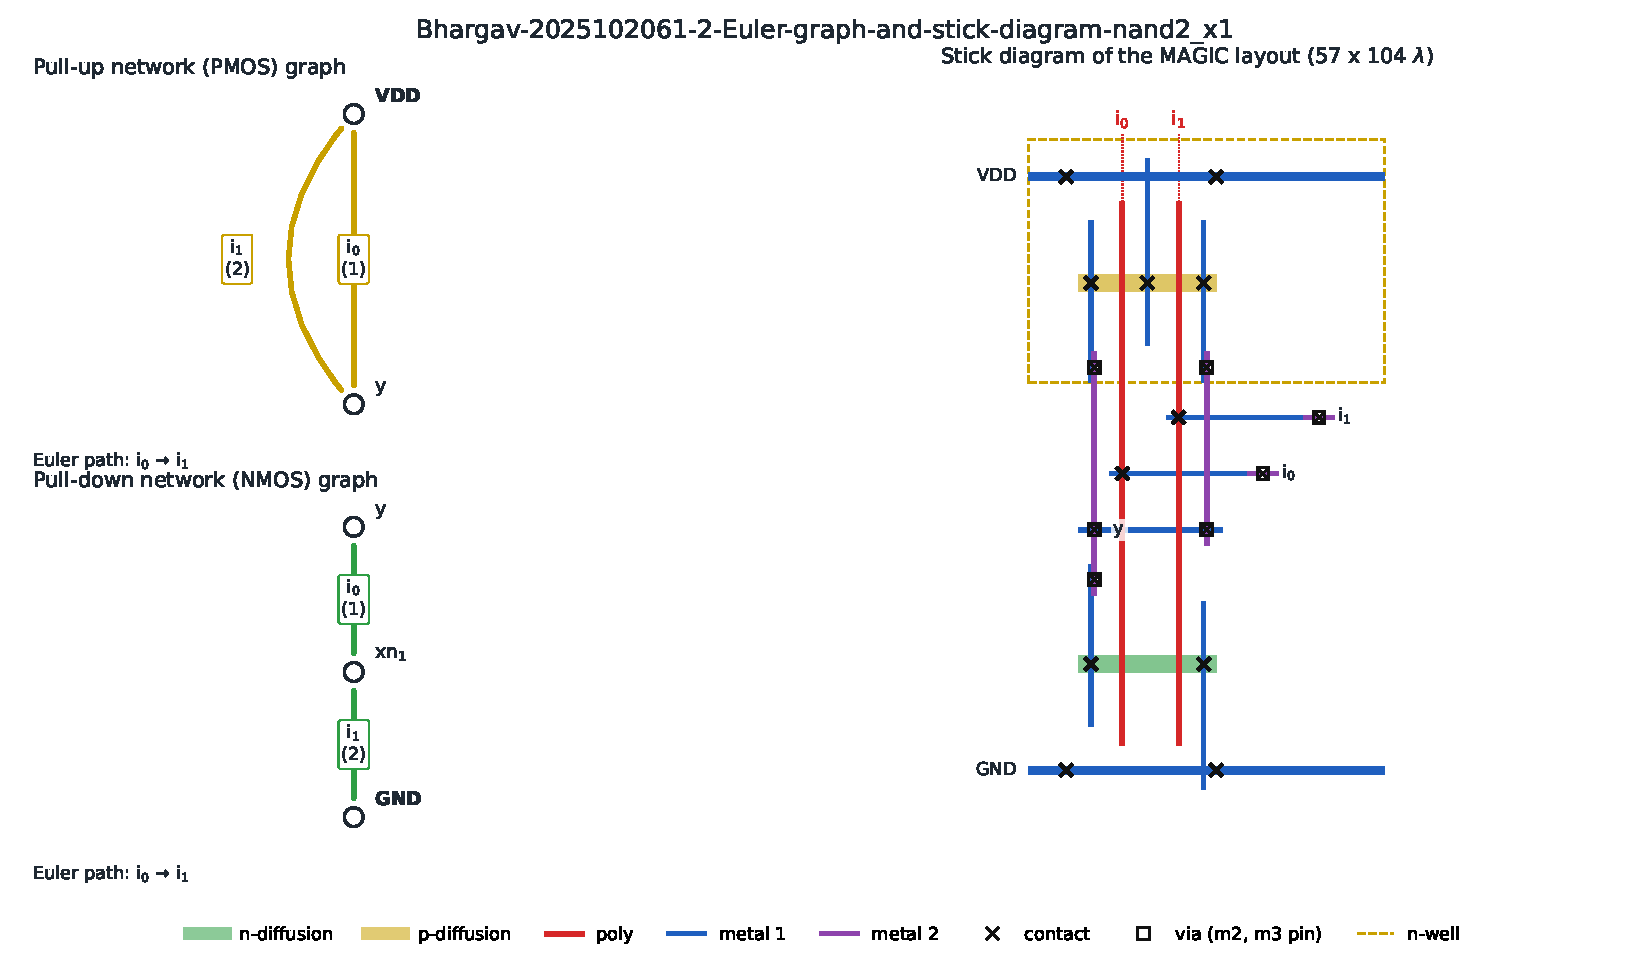
\includegraphics[width=\textwidth]{figures/stick_nand2_x1.pdf}\caption{Euler graphs of the pull-up and pull-down networks, and stick diagram of the MAGIC layout: NAND2.}\end{figure*}

\begin{figure*}[!t]\centering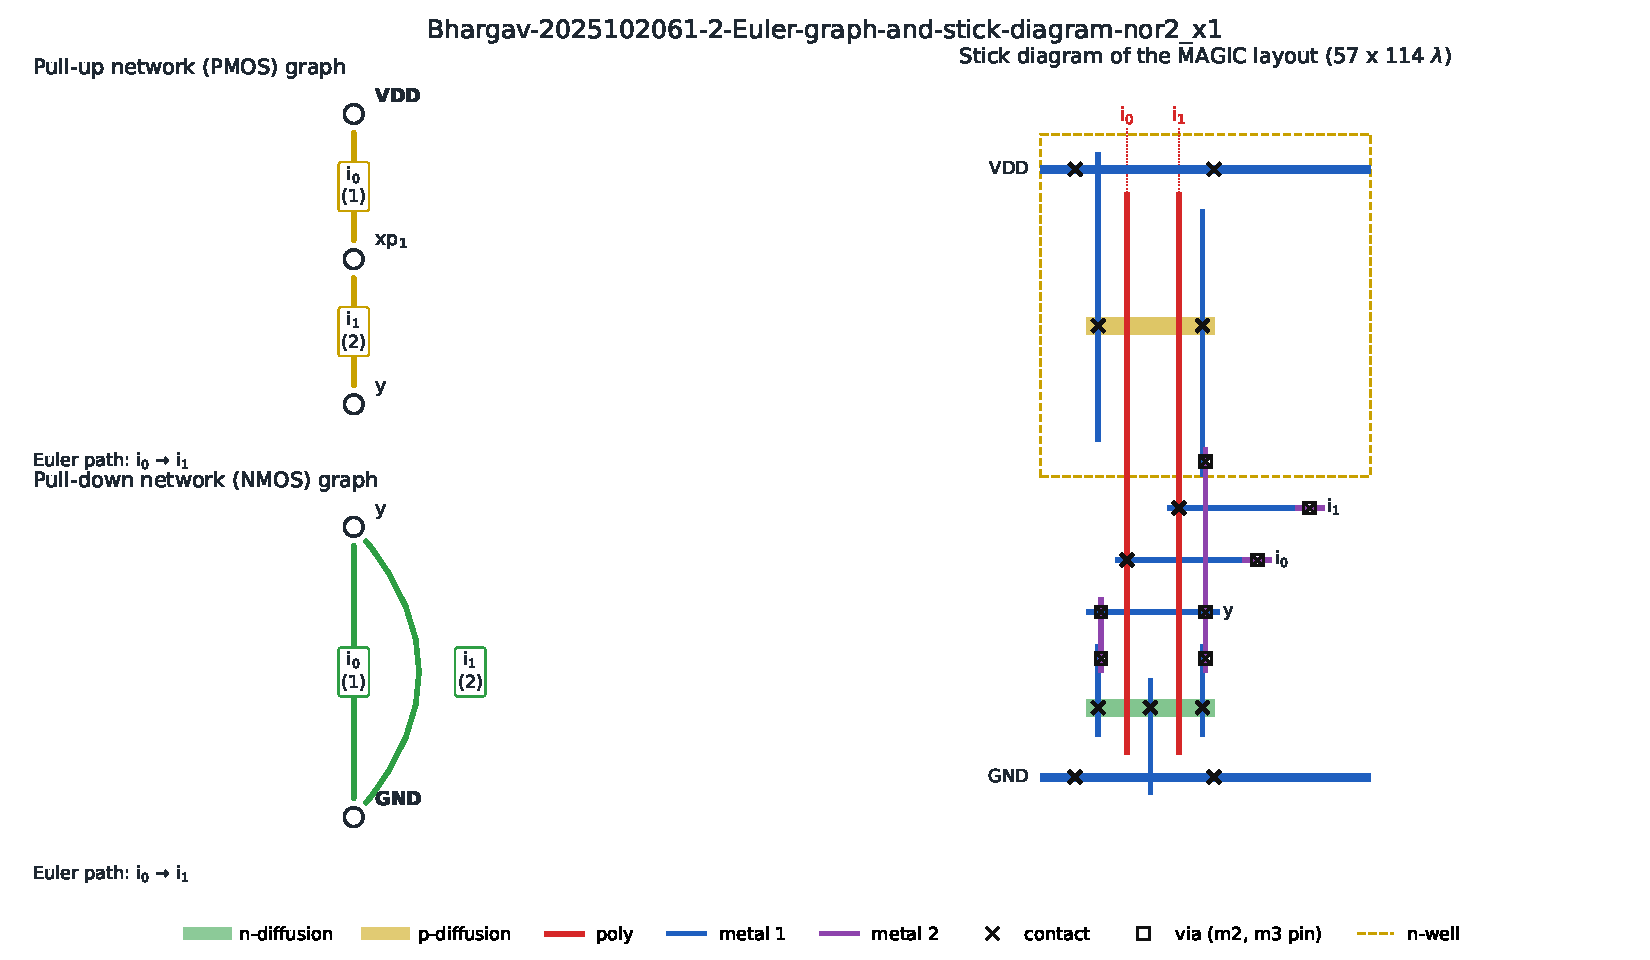
\includegraphics[width=\textwidth]{figures/stick_nor2_x1.pdf}\caption{Euler graphs of the pull-up and pull-down networks, and stick diagram of the MAGIC layout: NOR2.}\end{figure*}

\begin{figure*}[!t]\centering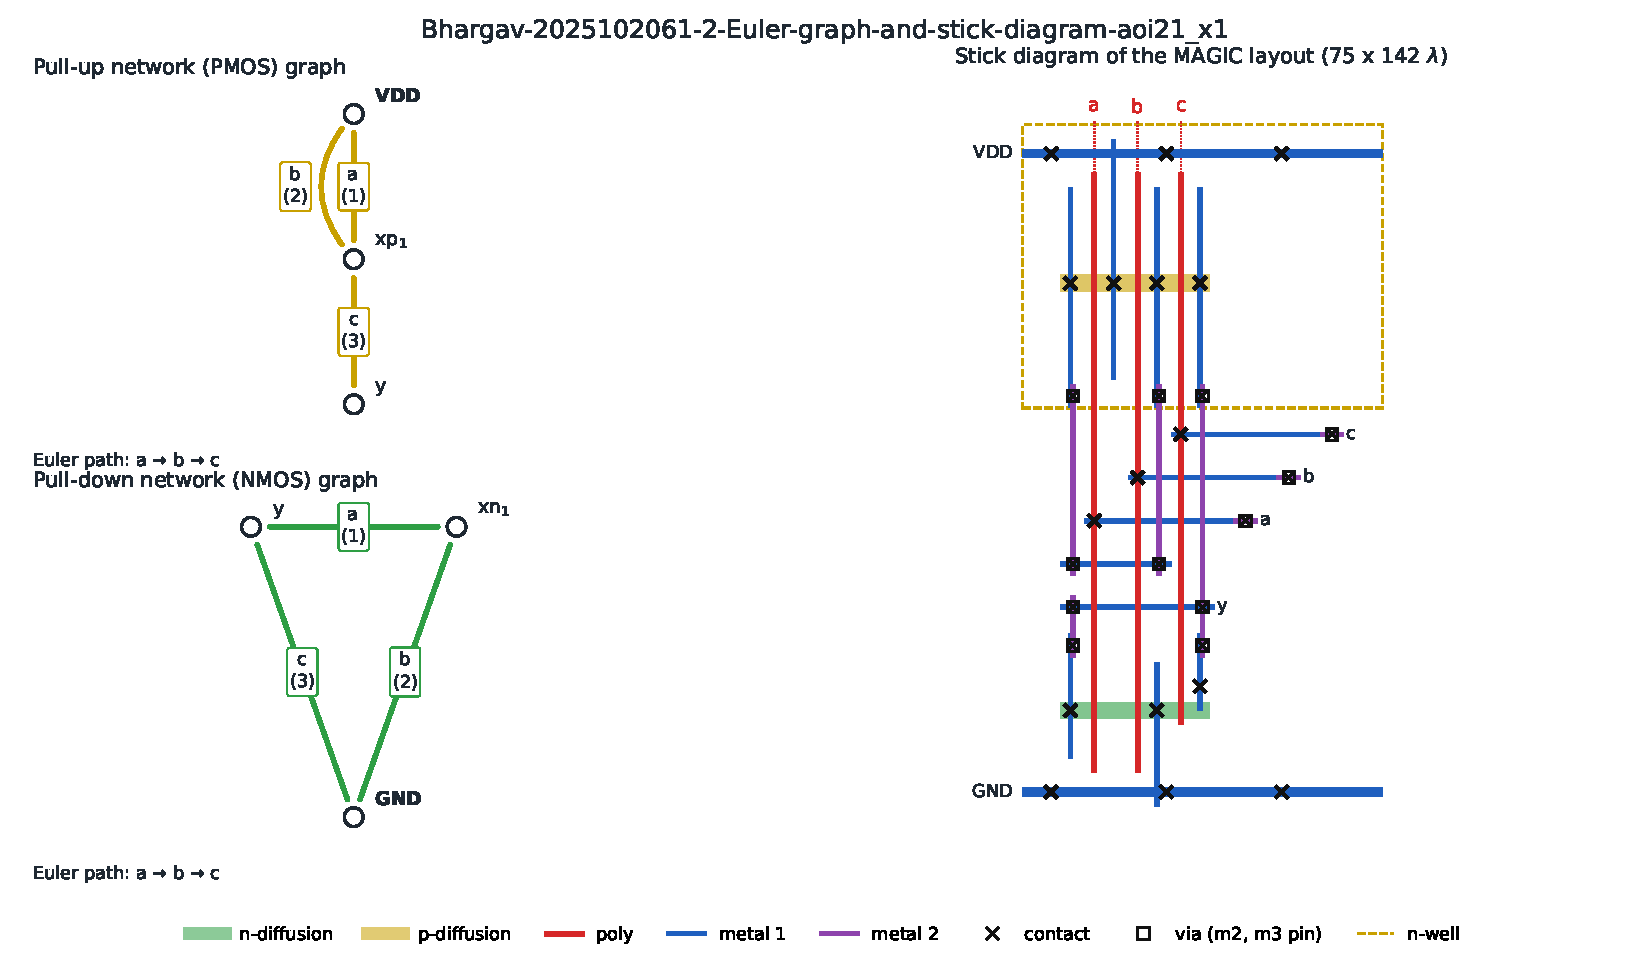
\includegraphics[width=\textwidth]{figures/stick_aoi21_x1.pdf}\caption{Euler graphs of the pull-up and pull-down networks, and stick diagram of the MAGIC layout: AOI21.}\end{figure*}

\begin{figure*}[!t]\centering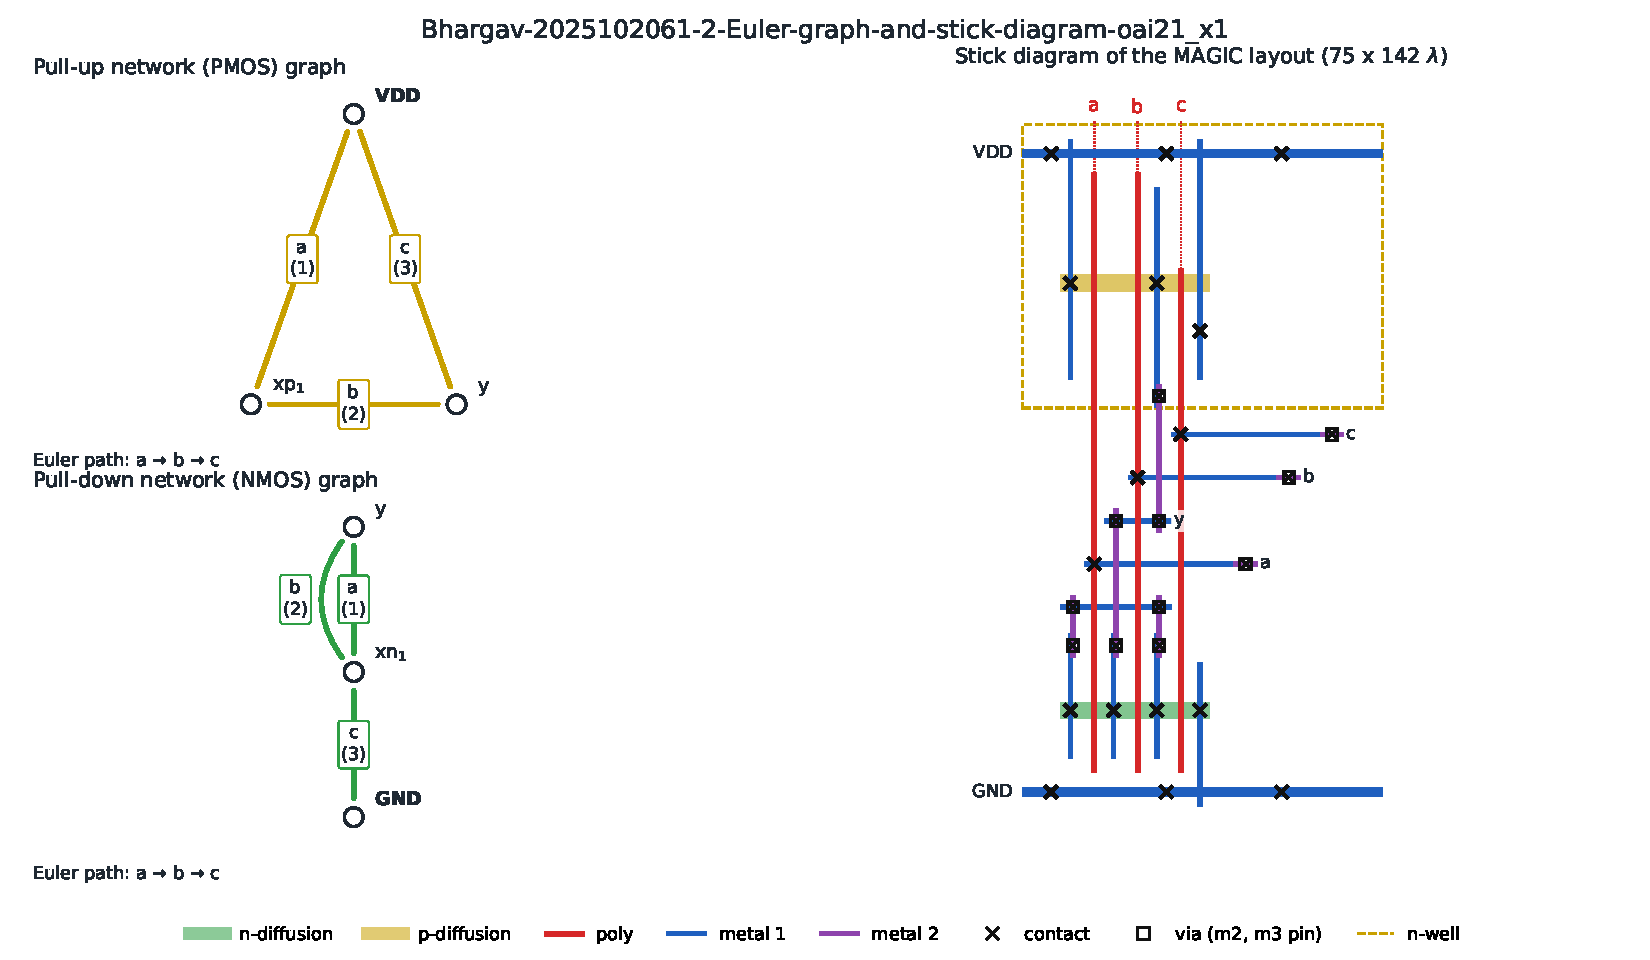
\includegraphics[width=\textwidth]{figures/stick_oai21_x1.pdf}\caption{Euler graphs of the pull-up and pull-down networks, and stick diagram of the MAGIC layout: OAI21.}\end{figure*}

\begin{figure*}[!t]\centering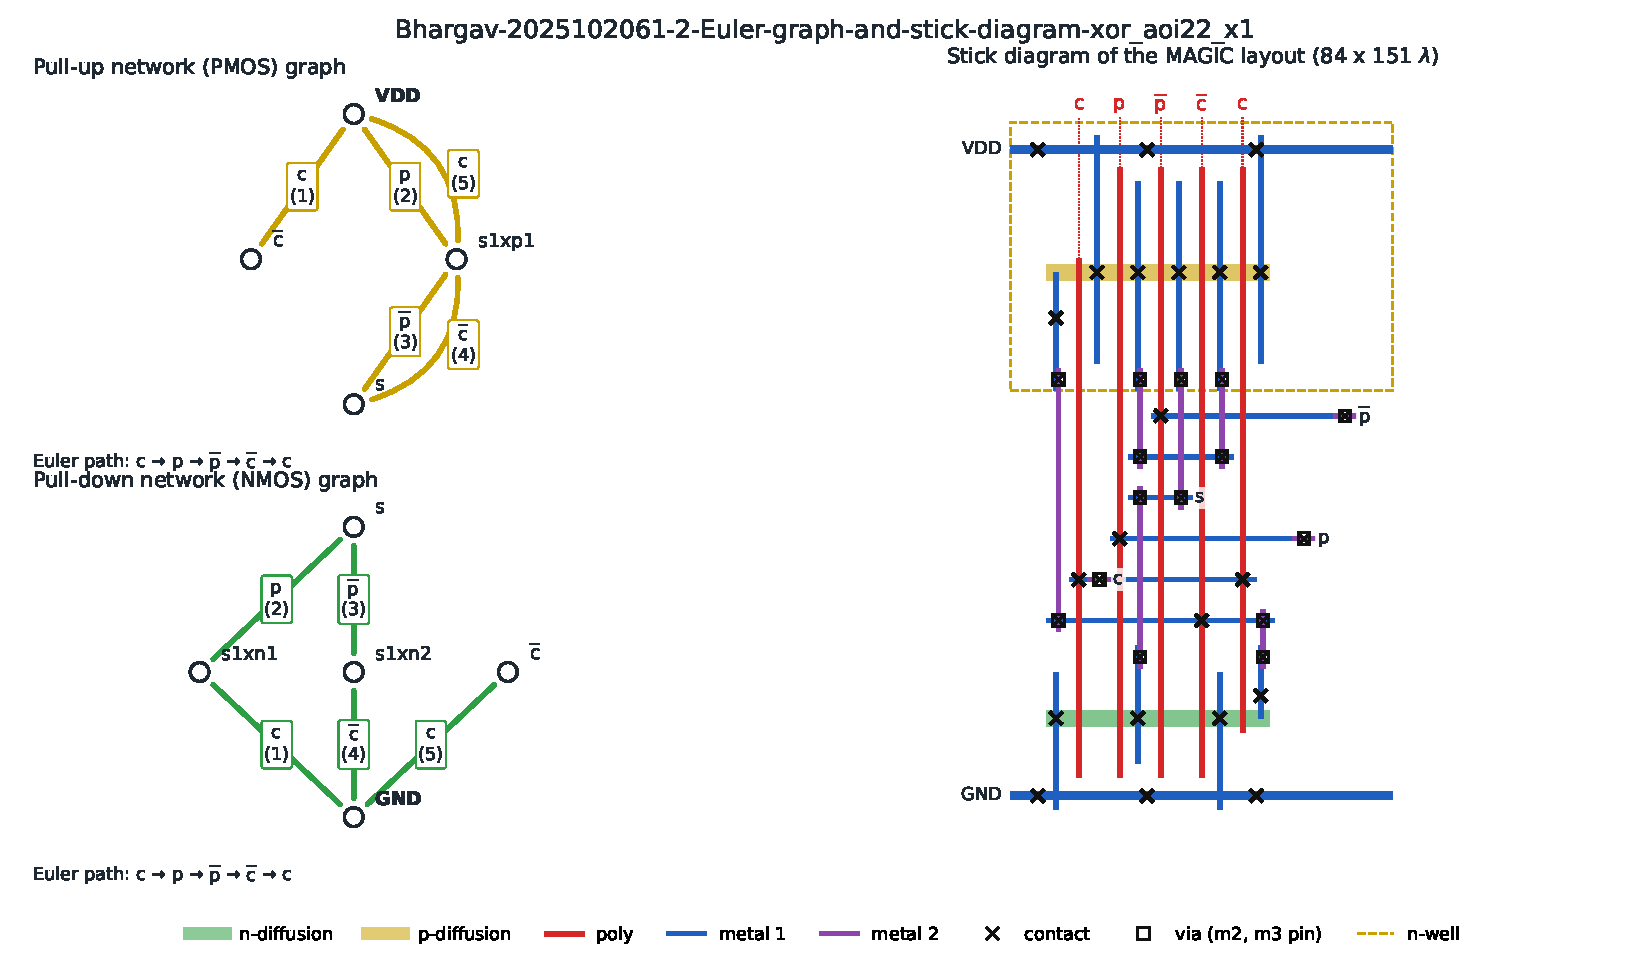
\includegraphics[width=\textwidth]{figures/stick_xor_aoi22_x1.pdf}\caption{Euler graphs of the pull-up and pull-down networks, and stick diagram of the MAGIC layout: AOI22 XOR (sum, with its carry inverter).}\end{figure*}

\begin{figure*}[!t]\centering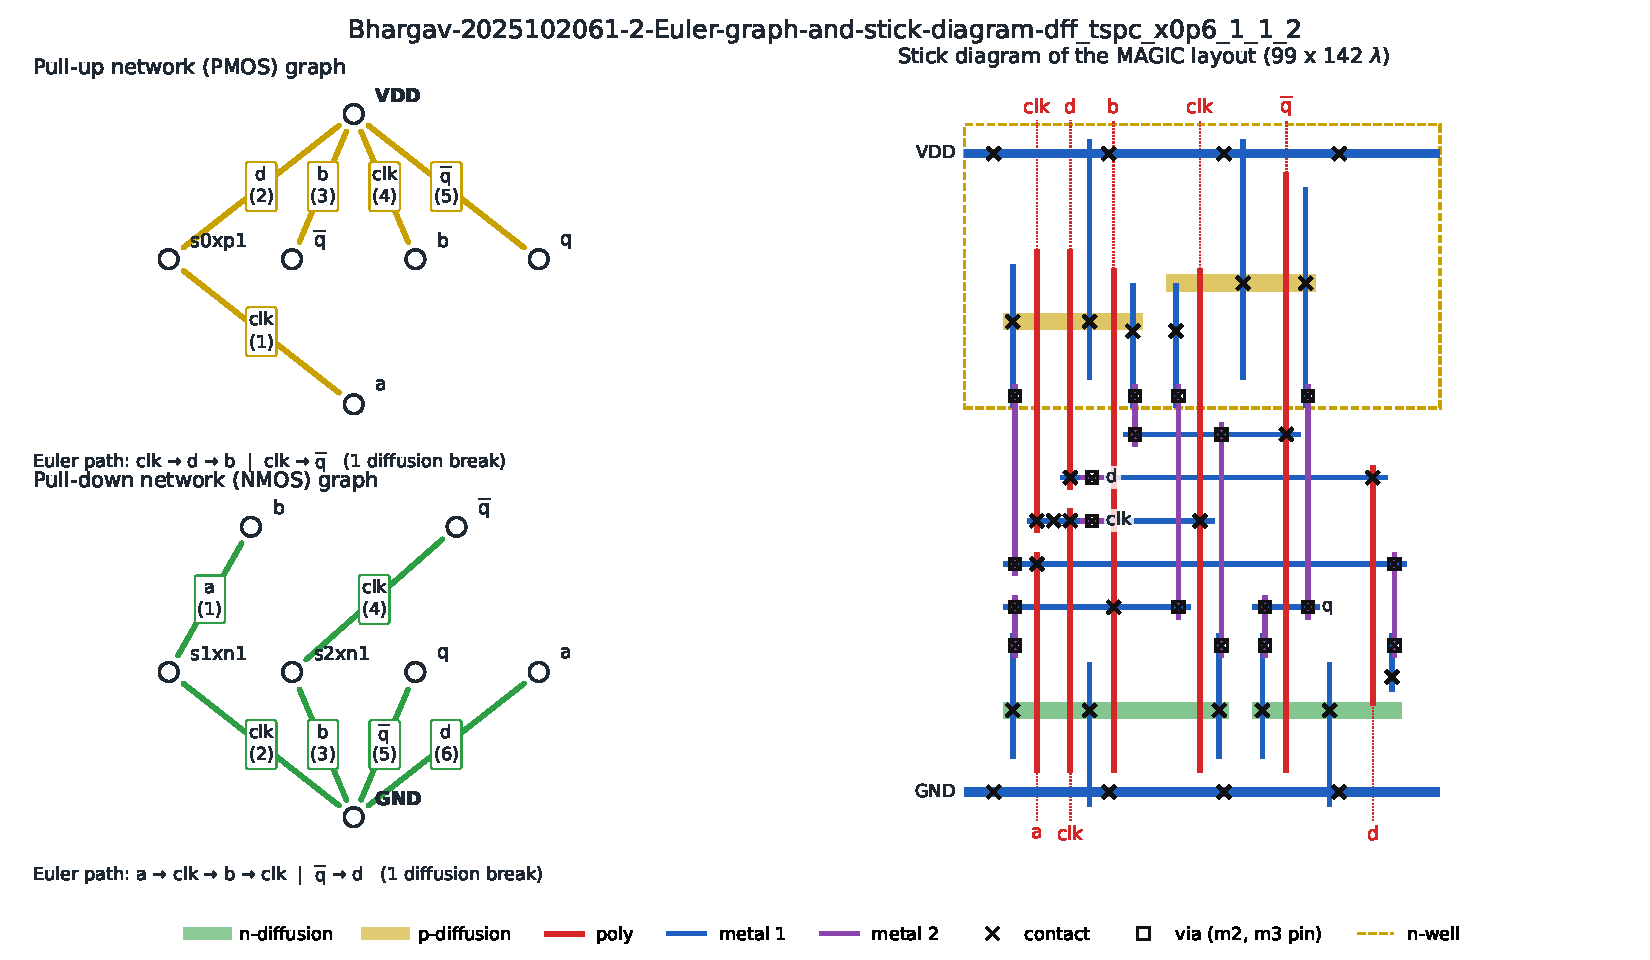
\includegraphics[width=\textwidth]{figures/stick_dff_tspc_x0p6_1_1_2.pdf}\caption{Euler graphs of the pull-up and pull-down networks, and stick diagram of the MAGIC layout: TSPC flip-flop.}\end{figure*}

\section{MAGIC Layouts}\label{sec:magic}
Every layout below is a screenshot of MAGIC's own layout window. Each cell passes MAGIC's DRC with zero errors, and each extracted netlist matches the schematic in LVS. Post-layout plots use the netlist MAGIC extracted, with all parasitic capacitance.

\subsection{Inverter}

\begin{figure}[H]\centering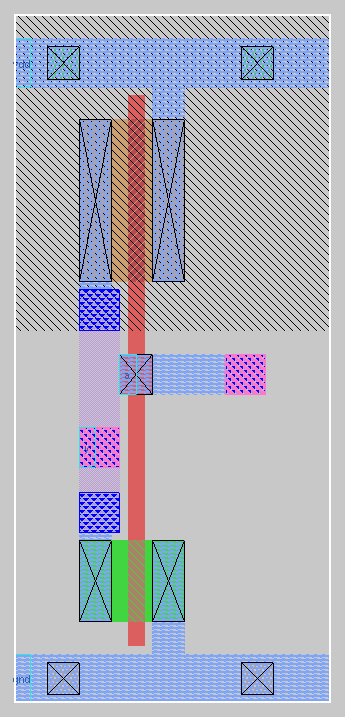
\includegraphics[width=0.36\columnwidth]{figures/magic_gate_inv_x1.png}\caption{MAGIC layout of Inverter.}\end{figure}

\begin{figure}[H]\centering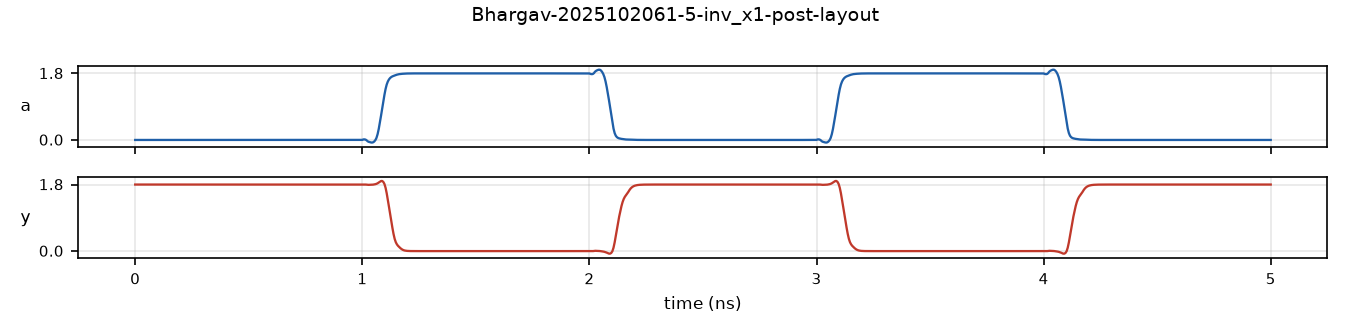
\includegraphics[width=\columnwidth]{figures/gate_inv_x1_post-layout.png}\caption{Inverter plot: post-layout.}\end{figure}

\subsection{NAND2}

\begin{figure}[H]\centering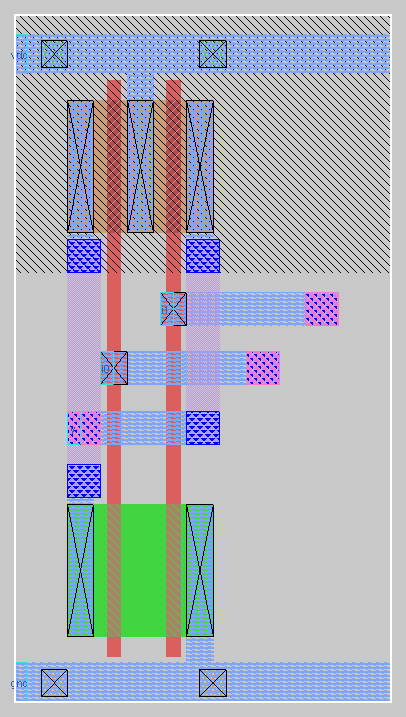
\includegraphics[width=0.36\columnwidth]{figures/magic_gate_nand2_x1.png}\caption{MAGIC layout of NAND2.}\end{figure}

\begin{figure}[H]\centering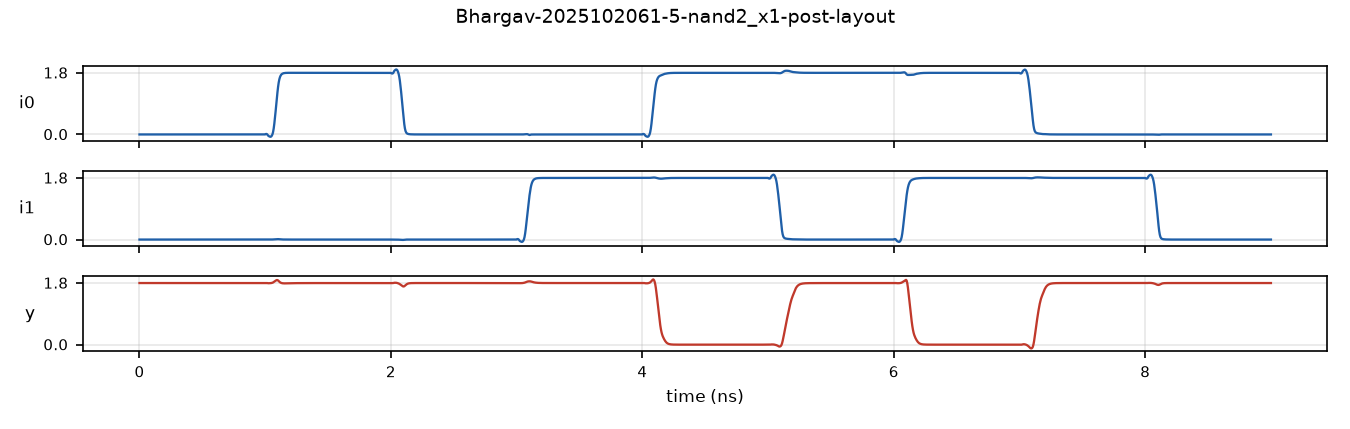
\includegraphics[width=\columnwidth]{figures/gate_nand2_x1_post-layout.png}\caption{NAND2 plot: post-layout.}\end{figure}

\subsection{NOR2}

\begin{figure}[H]\centering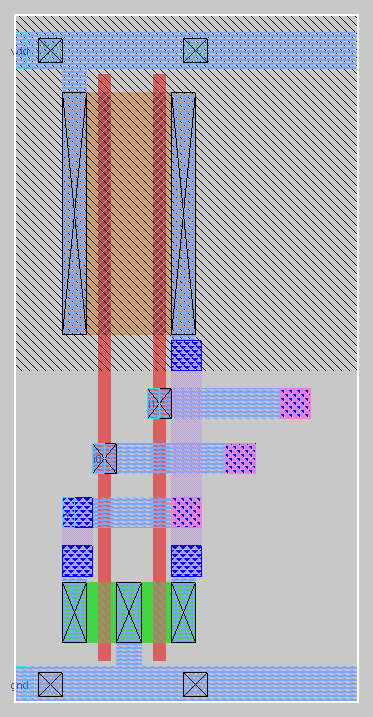
\includegraphics[width=0.36\columnwidth]{figures/magic_gate_nor2_x1.png}\caption{MAGIC layout of NOR2.}\end{figure}

\begin{figure}[H]\centering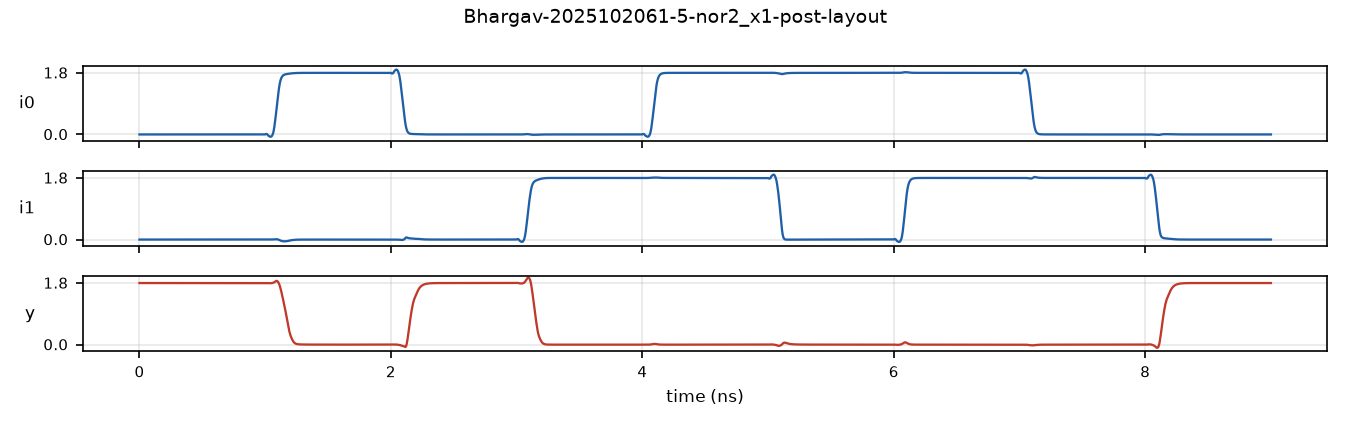
\includegraphics[width=\columnwidth]{figures/gate_nor2_x1_post-layout.png}\caption{NOR2 plot: post-layout.}\end{figure}

\subsection{AOI21}

\begin{figure}[H]\centering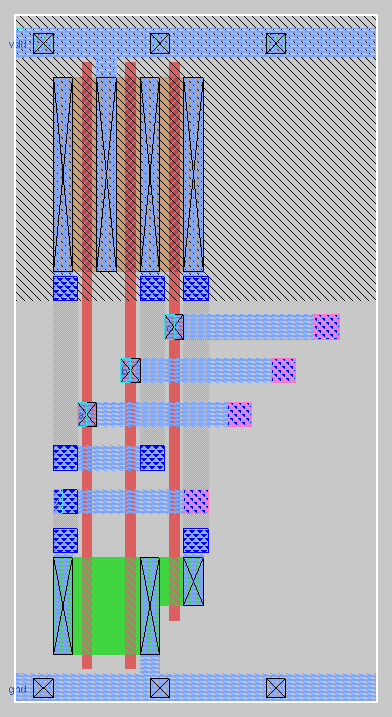
\includegraphics[width=0.36\columnwidth]{figures/magic_gate_aoi21_x1.png}\caption{MAGIC layout of AOI21.}\end{figure}

\begin{figure}[H]\centering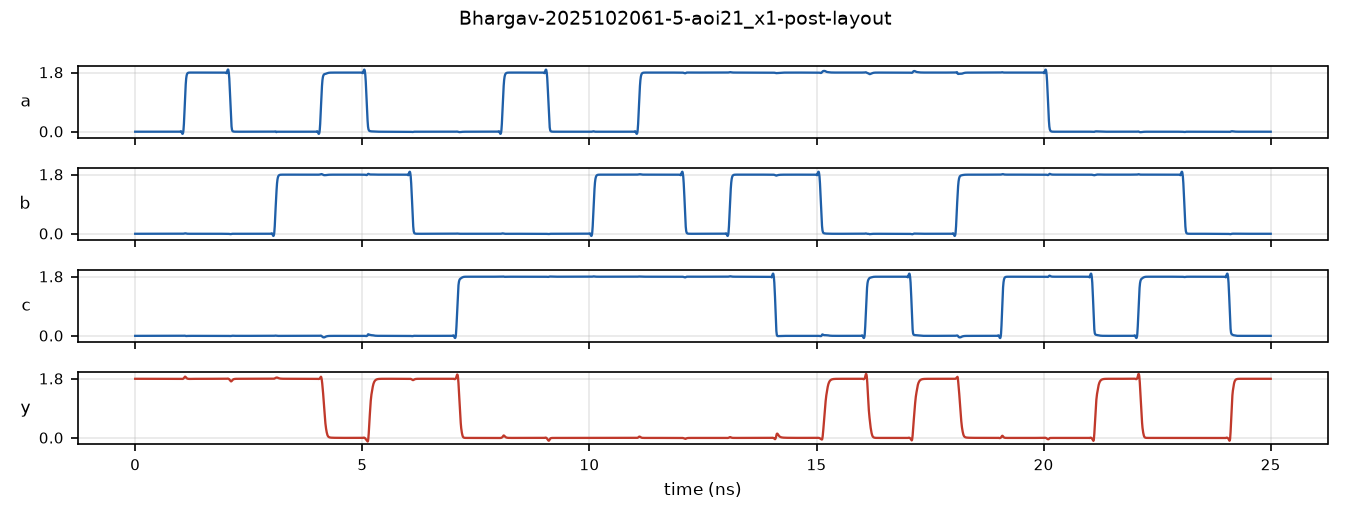
\includegraphics[width=\columnwidth]{figures/gate_aoi21_x1_post-layout.png}\caption{AOI21 plot: post-layout.}\end{figure}

\subsection{OAI21}

\begin{figure}[H]\centering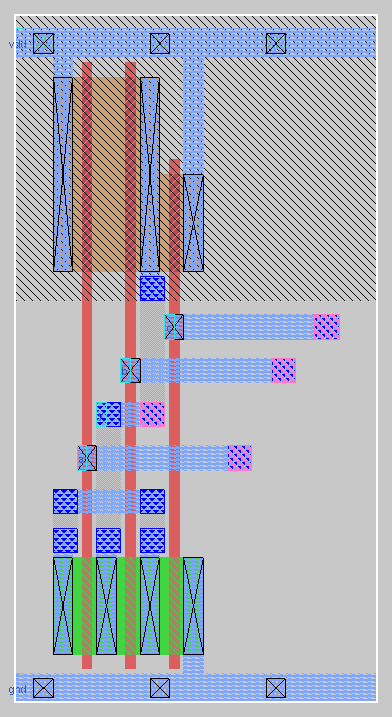
\includegraphics[width=0.36\columnwidth]{figures/magic_gate_oai21_x1.png}\caption{MAGIC layout of OAI21.}\end{figure}

\begin{figure}[H]\centering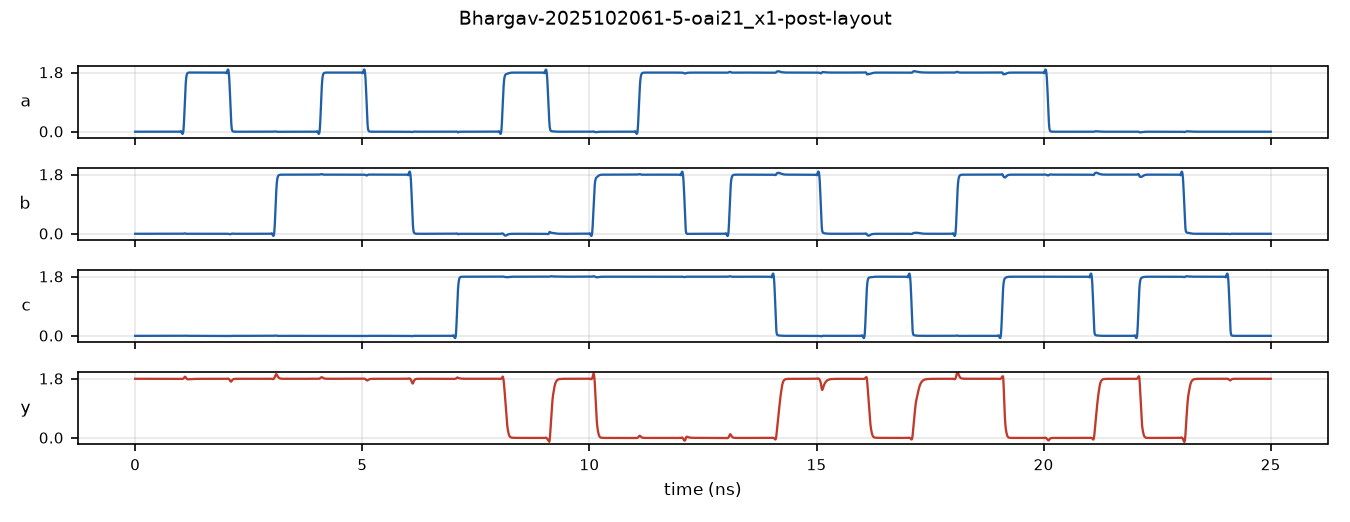
\includegraphics[width=\columnwidth]{figures/gate_oai21_x1_post-layout.png}\caption{OAI21 plot: post-layout.}\end{figure}

\subsection{AOI22 XOR (sum)}

\begin{figure}[H]\centering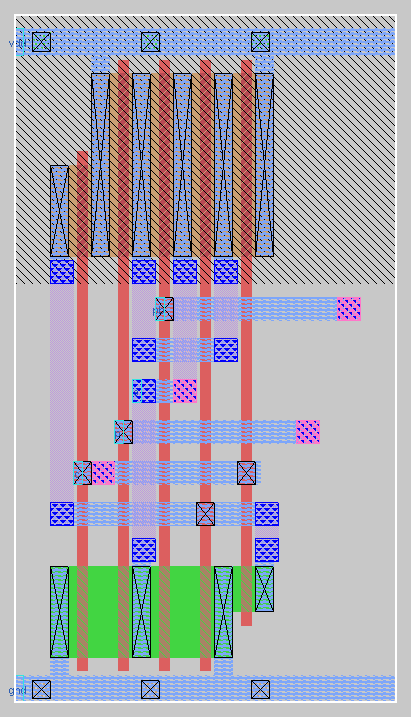
\includegraphics[width=0.36\columnwidth]{figures/magic_gate_xor_aoi22_x1.png}\caption{MAGIC layout of AOI22 XOR (sum).}\end{figure}

\begin{figure}[H]\centering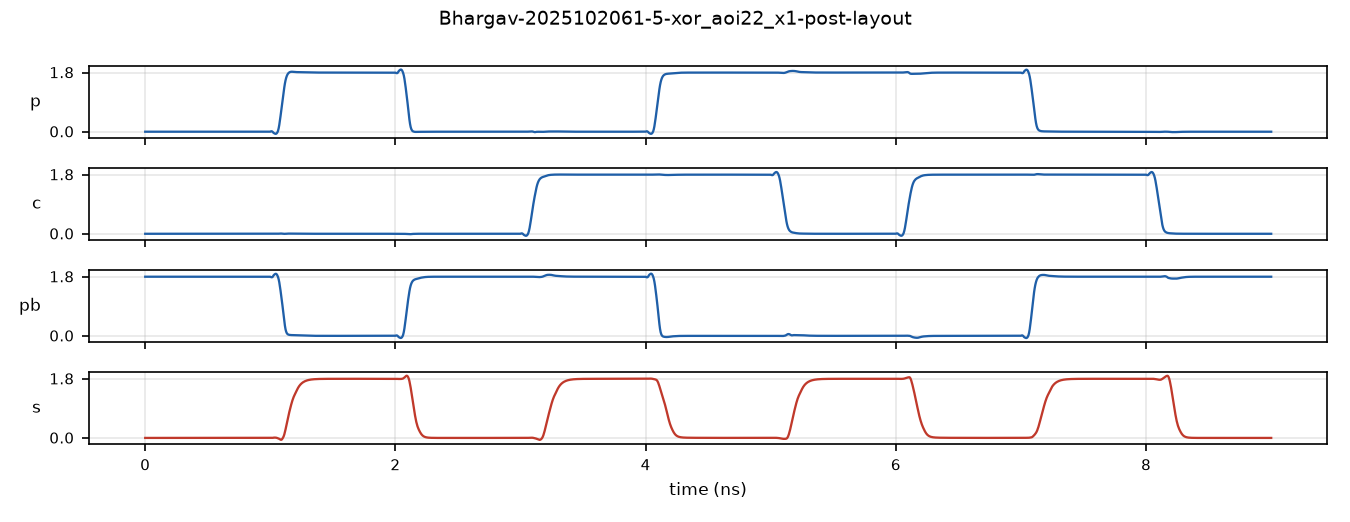
\includegraphics[width=\columnwidth]{figures/gate_xor_aoi22_x1_post-layout.png}\caption{AOI22 XOR (sum) plot: post-layout.}\end{figure}

\subsection{D Flip-Flop}

\begin{figure}[H]\centering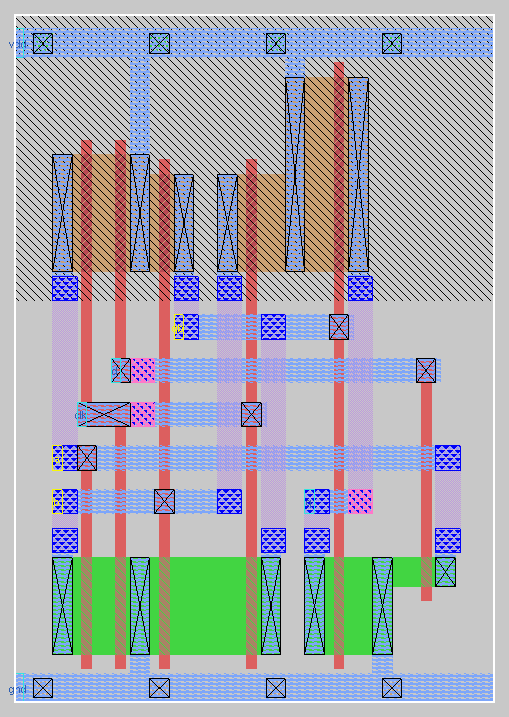
\includegraphics[width=0.45\columnwidth]{figures/magic_gate_dff.png}\caption{MAGIC layout of the TSPC D flip-flop.}\end{figure}

\begin{figure}[H]\centering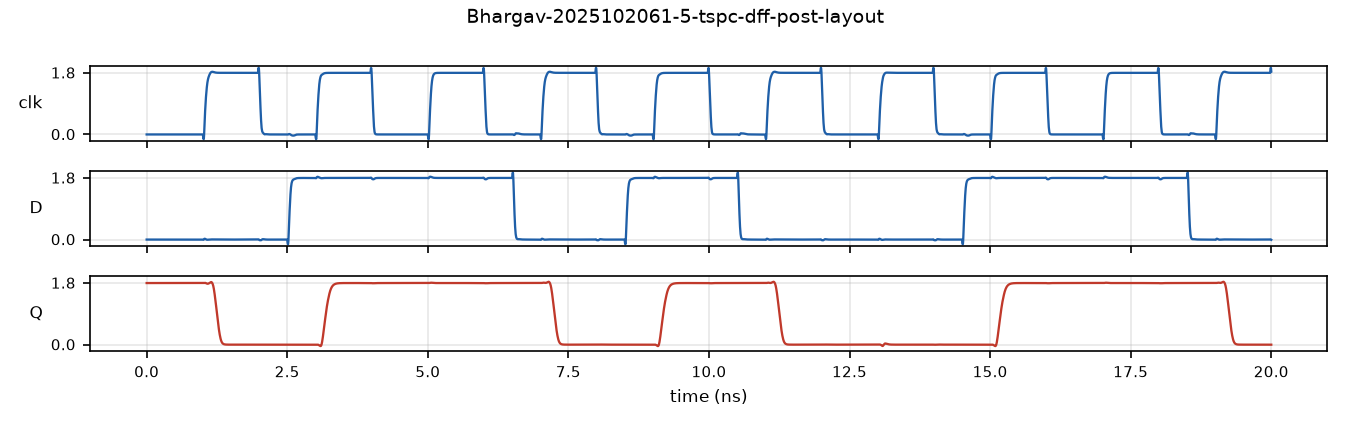
\includegraphics[width=\columnwidth]{figures/dff_post-layout.png}\caption{TSPC D flip-flop plot: post-layout.}\end{figure}

\subsection{Clock to Q, Set Up and Hold Time of the Flip-Flop}

\begin{table}[H]\centering\footnotesize
\caption{Flip-flop timing, pre- and post-layout}
\begin{tabular}{|c|c|c|}\hline
Parameter (ps) & Pre-layout & Post-layout \\ \hline
$t_{cq}$ & 208.5 & 204.2 \\ \hline
$t_{su}$ & 34.0 & 38.0 \\ \hline
$t_{hold}$ & 55.1 & 45.7 \\ \hline
\end{tabular}
\end{table}

\subsection{P/G Block}

\begin{figure}[H]\centering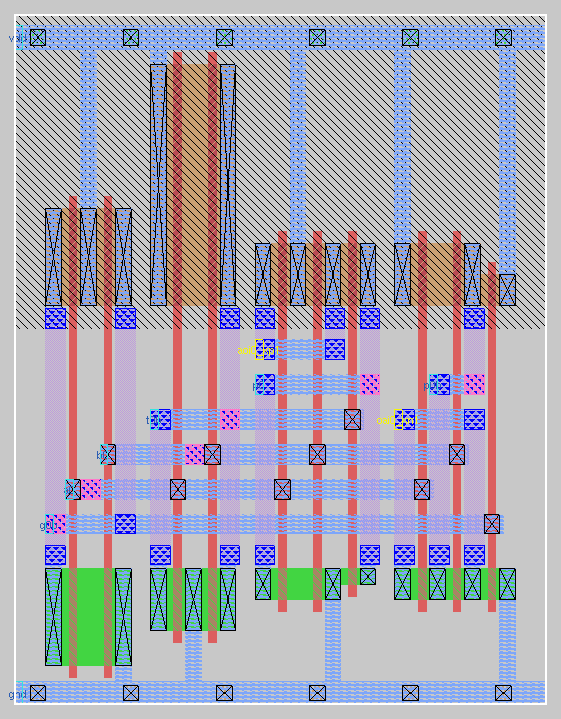
\includegraphics[width=0.45\columnwidth]{figures/magic_block_pg0_b.png}\caption{MAGIC layout of the P/G Block.}\end{figure}

\begin{figure}[H]\centering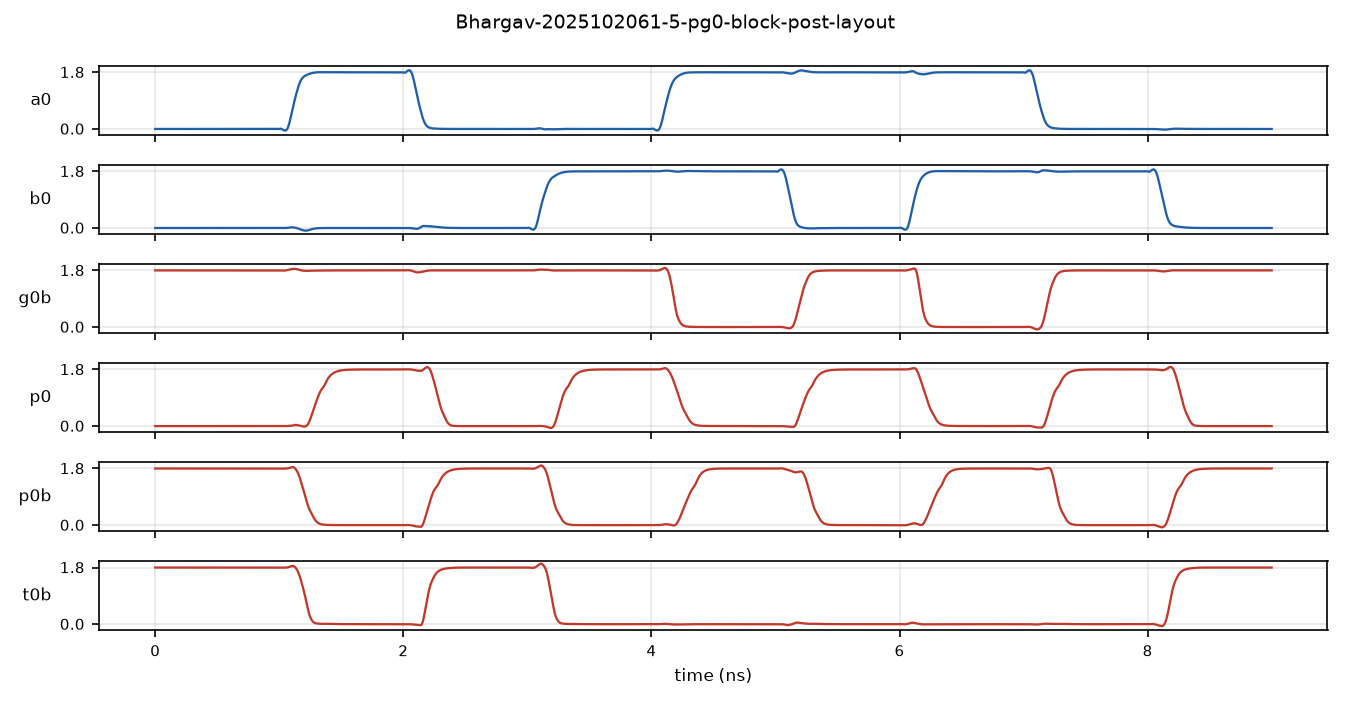
\includegraphics[width=\columnwidth]{figures/block_pg0_post-layout.png}\caption{P/G Block plot: post-layout.}\end{figure}

\subsection{Carry Block}

\begin{figure}[H]\centering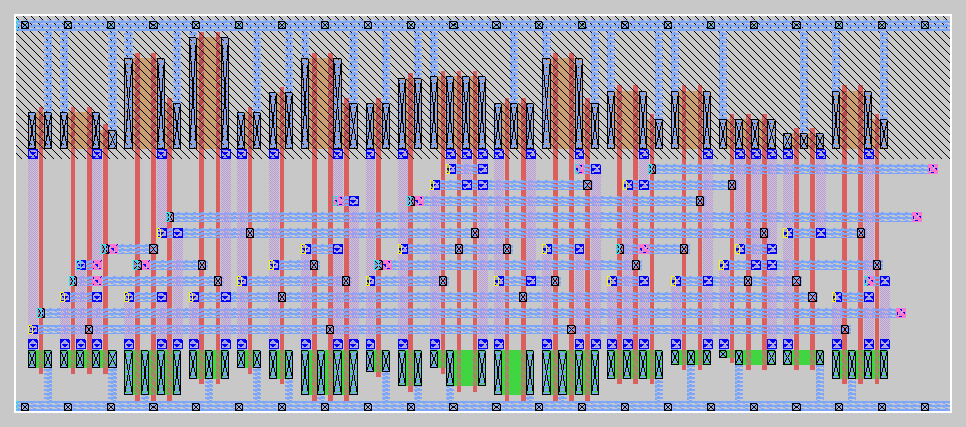
\includegraphics[width=0.95\columnwidth]{figures/magic_block_carry_b.png}\caption{MAGIC layout of the Carry Block.}\end{figure}

\begin{figure}[H]\centering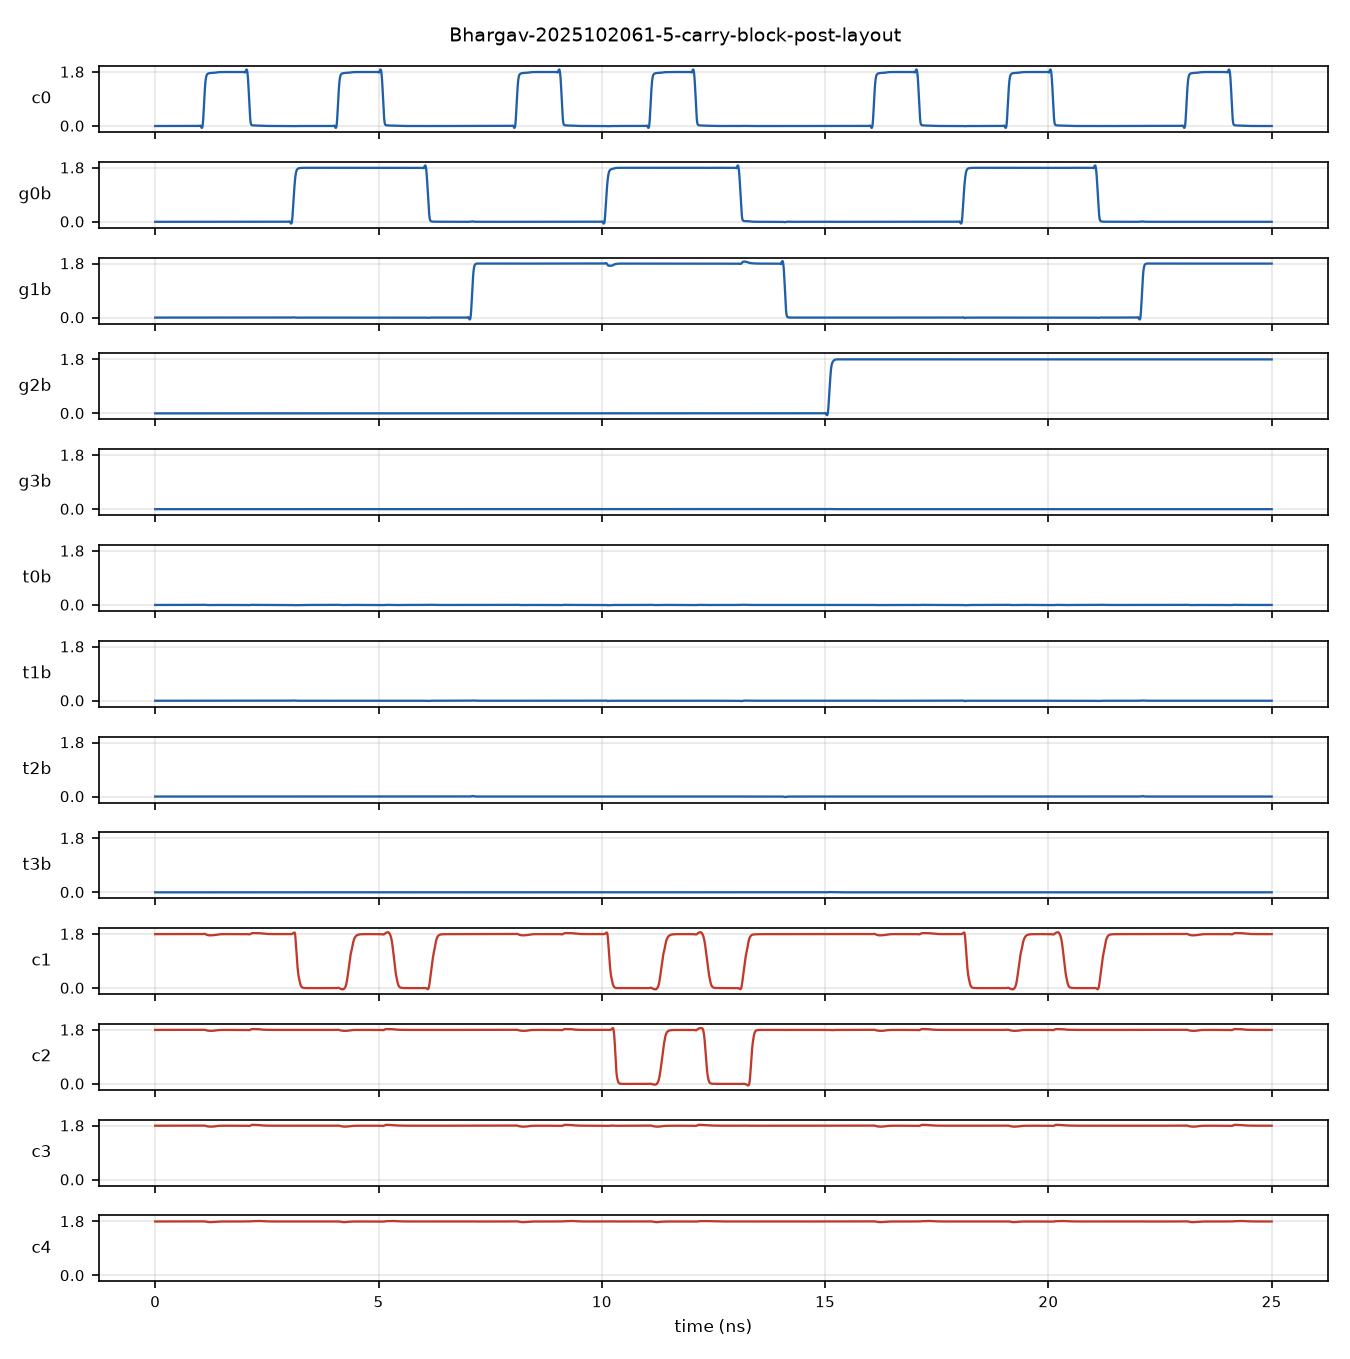
\includegraphics[width=\columnwidth]{figures/block_carry_post-layout.png}\caption{Carry Block plot: post-layout.}\end{figure}

\subsection{Sum Block}

\begin{figure}[H]\centering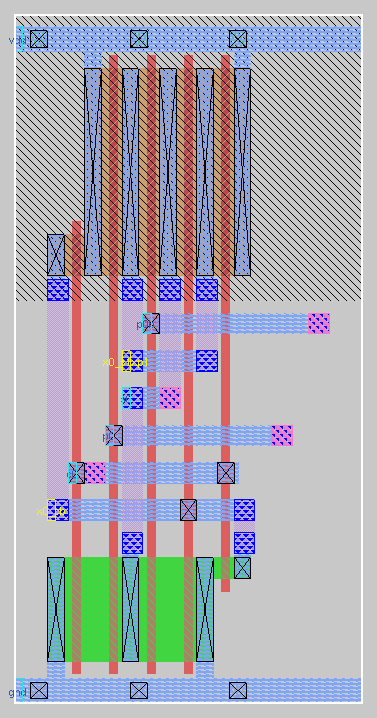
\includegraphics[width=0.45\columnwidth]{figures/magic_block_sum0_b.png}\caption{MAGIC layout of the Sum Block.}\end{figure}

\begin{figure}[H]\centering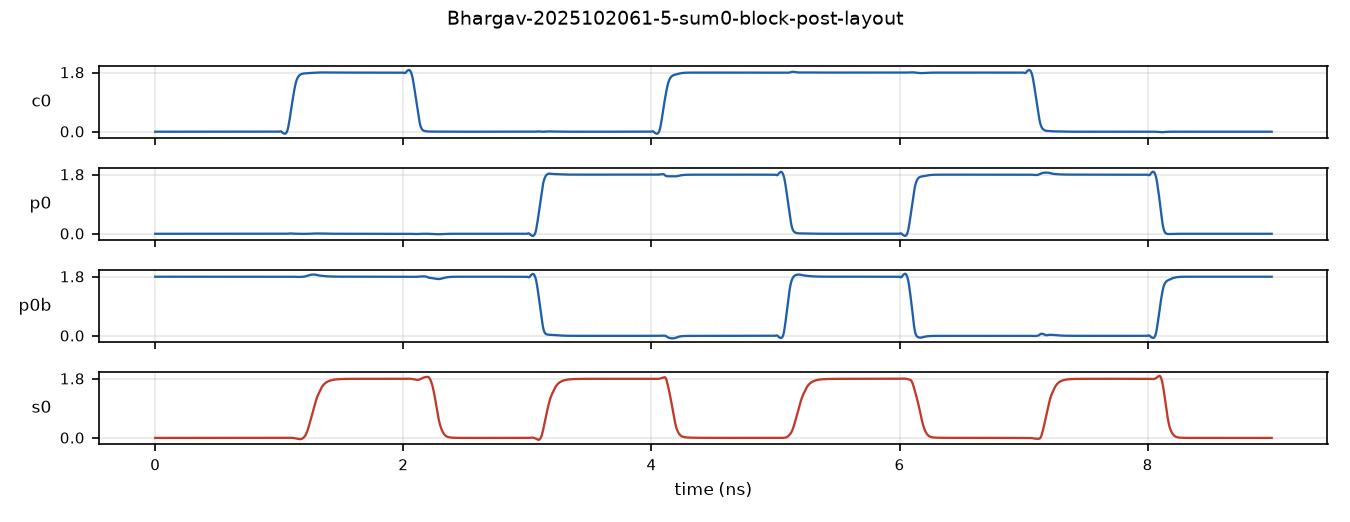
\includegraphics[width=\columnwidth]{figures/block_sum0_post-layout.png}\caption{Sum Block plot: post-layout.}\end{figure}

\begin{table}[H]\centering\scriptsize
\caption{Gates and blocks: pre-layout against post-layout. Block delays are worst over all their single-input transitions.}
\begin{tabular}{|c|c|c|c|c|}\hline
Cell & Pre tpLH & Pre tpHL & Post tpLH & Post tpHL \\ \hline
Inverter & 38.59 & 35.7 & 39.4 & 36.47 \\ \hline
NAND2 & 66.02 & 45.44 & 66.14 & 45.9 \\ \hline
NOR2 & 64.35 & 70.61 & 64.67 & 70.81 \\ \hline
AOI21 & 91.52 & 74.76 & 88.88 & 71.15 \\ \hline
OAI21 & 92.91 & 75.84 & 84.86 & 69.97 \\ \hline
AOI22 XOR (sum) & 134.99 & 122.89 & 135.36 & 122.15 \\ \hline
block pg0 & 187.21 & 168.95 & 201.02 & 176.08 \\ \hline
block pg1 & 187.4 & 171.1 & 200.97 & 169.7 \\ \hline
block pg2 & 195.19 & 176.14 & 206.87 & 180.24 \\ \hline
block pg3 & 199.86 & 189.09 & 210.24 & 190.19 \\ \hline
block carry & 319.87 & 306.42 & 335.79 & 336.37 \\ \hline
block sum0 & 176.33 & 173.69 & 182.49 & 171.72 \\ \hline
block sum1 & 157.14 & 144.1 & 161.33 & 142.78 \\ \hline
block sum2 & 134.23 & 119.06 & 134.85 & 118.7 \\ \hline
block sum3 & 134.71 & 114.42 & 137.22 & 117.54 \\ \hline
\end{tabular}
\end{table}

Pre- and post-layout plots match for every gate and block. Delays change little at cell level, because a single cell has short wires; the difference grows once the cells are wired together (Section XI).

\section{NGSPICE Circuit (Pre-Layout)}
The full circuit of the course's Figure 1(i) has 9 input flip-flops ($a$, $b$ and $c_0$), the adder and 5 output flip-flops. A ninth flip-flop on $c_0$ keeps every input on the same clock. Inputs change before a rising edge; the sum appears at the output flip-flops one clock later.

\begin{figure*}[!t]\centering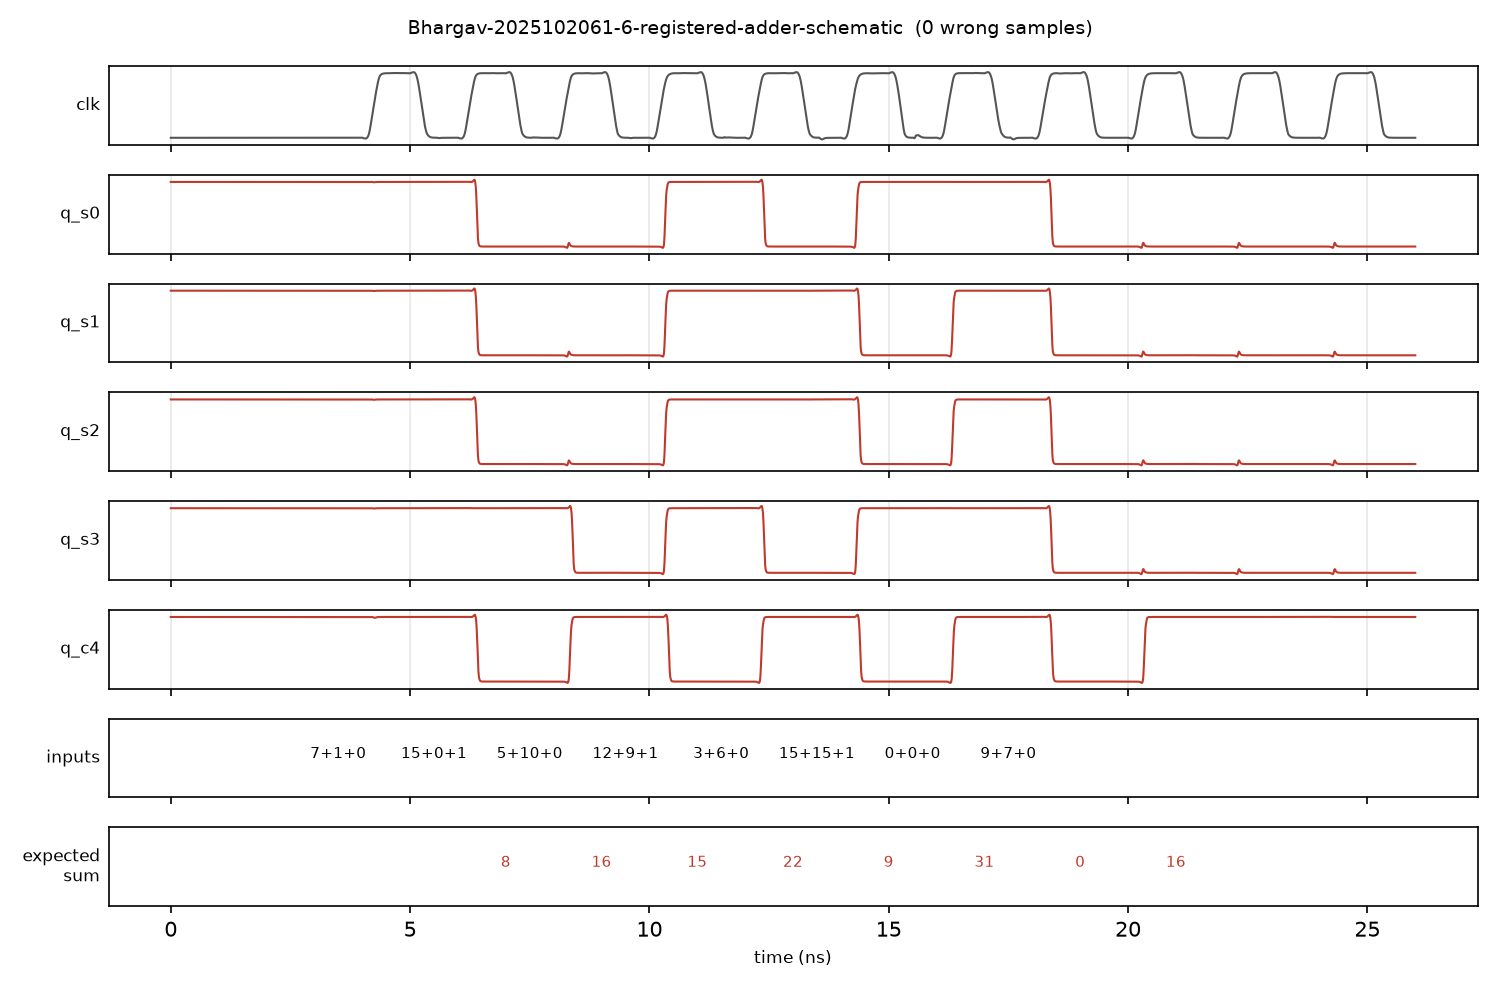
\includegraphics[width=0.9\textwidth]{figures/system_schematic.png}\caption{Registered adder plot: pre-layout. Each sum appears one clock after its inputs.}\end{figure*}

\textbf{Worst-case delay.} The worst case was found by search, not assumed: all 4608 single-input transitions, each timed to the last 50\% crossing so false sums cannot shorten it. Pre-layout worst: \textbf{516.30\,ps}, a1 rise to s3 rise, A=0101 B=0001 C0=0. The course hint vector, $A = 1111$, $B = 0000$ with $c_0$ toggling, gives only 377.45\,ps, because $c_0$ enters the prefix tree last.

\textbf{Clock.} The shortest clock at which the pre-layout registered circuit gave no wrong outputs on 264 vectors is 740.2\,ps, 1.351\,GHz.

\section{MAGIC Layout Plan}

\begin{figure}[H]\centering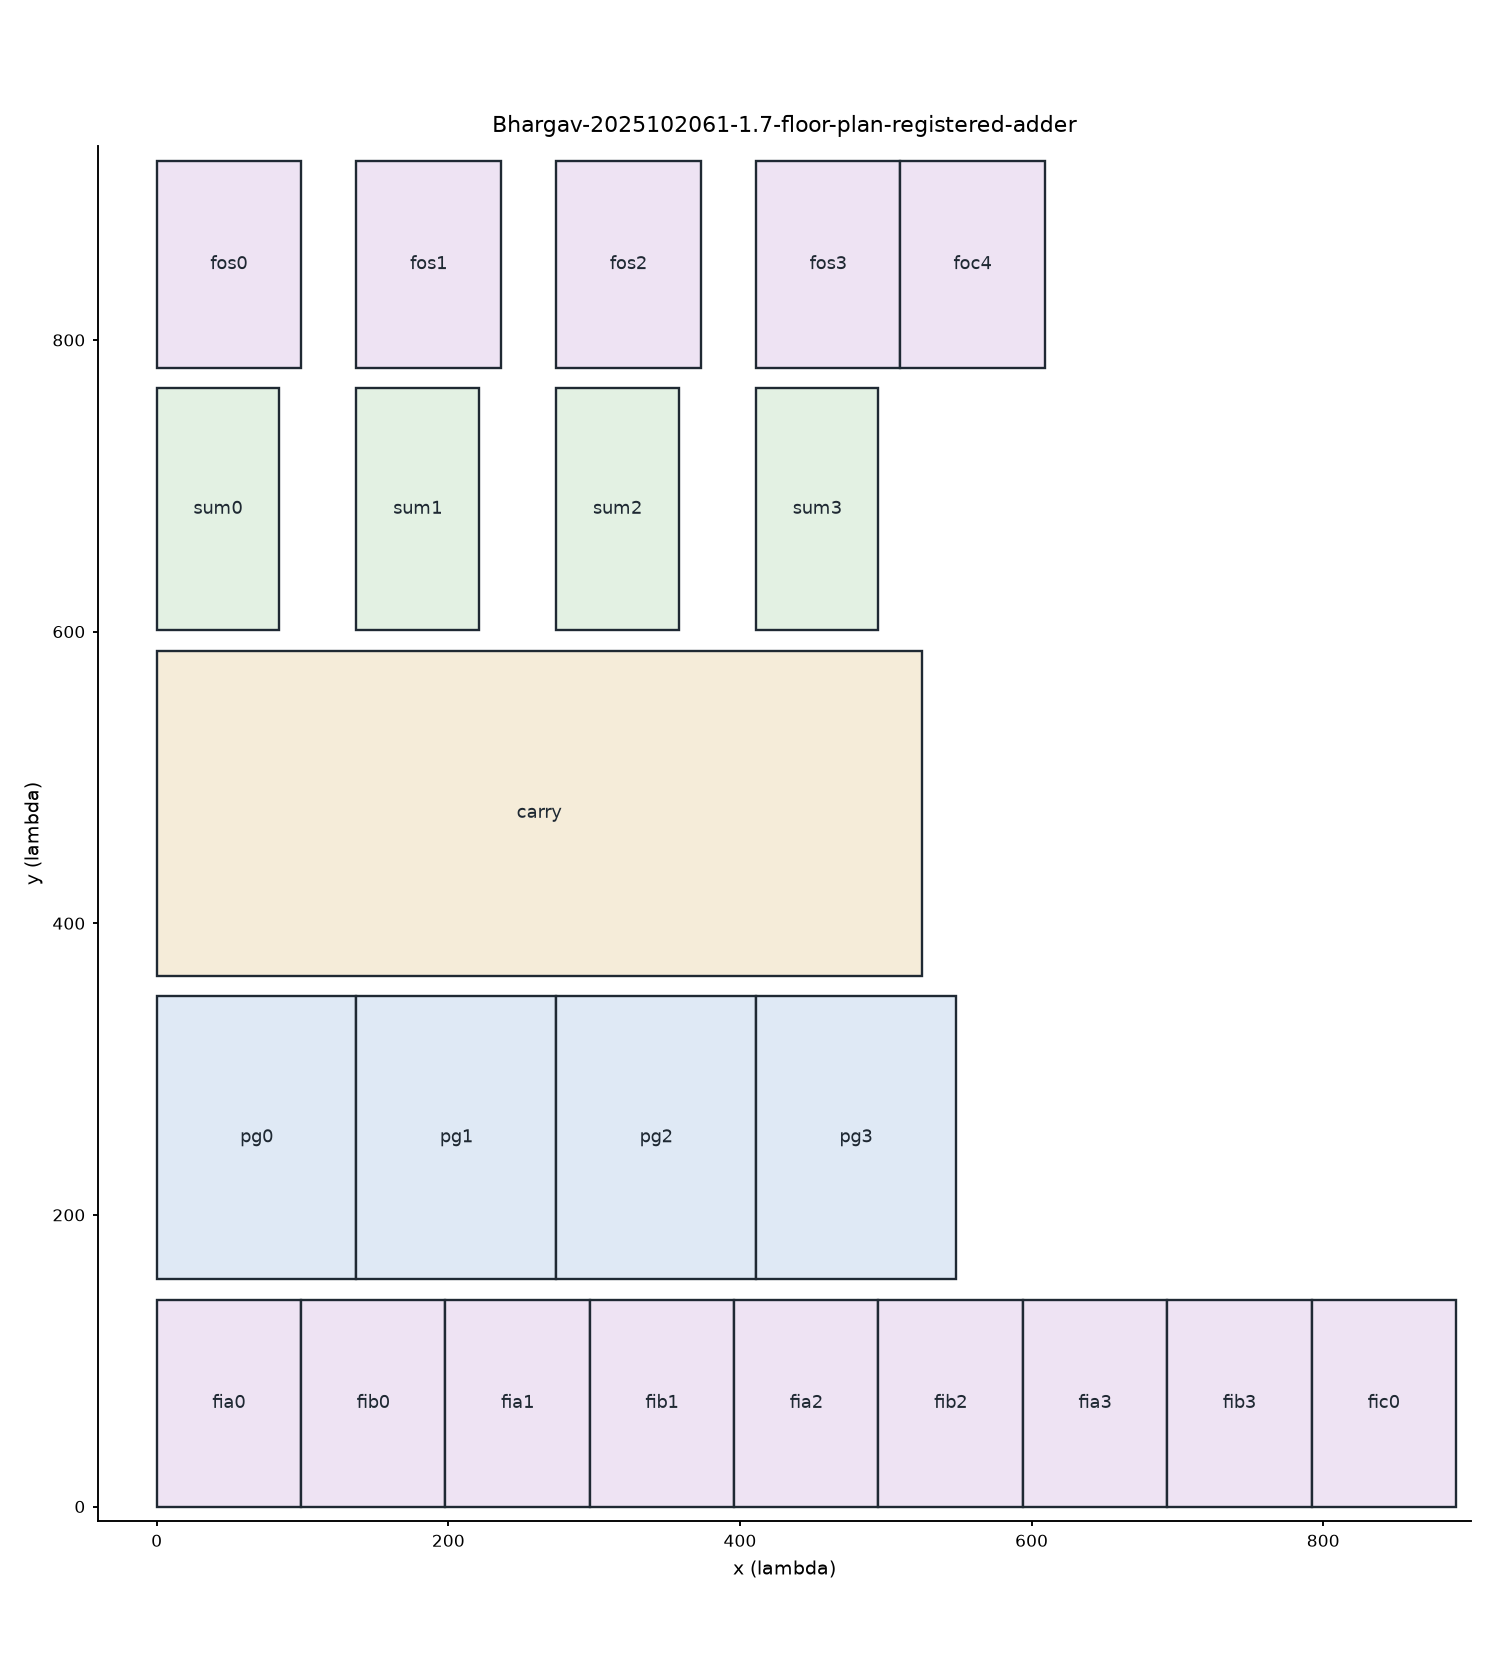
\includegraphics[width=\columnwidth]{figures/figures_floorplan.png}\caption{MAGIC layout floor plan. Rows from the bottom: input flip-flops, P/G bits, carry block, sum bits, output flip-flops.}\end{figure}

Signals flow upward through the rows. The P/G and sum cells sit on one bit pitch, so each sum bit lines up with its own P/G bit.

\begin{table}[H]\centering\footnotesize
\caption{Pitches}
\begin{tabular}{|c|c|c|}\hline
Pitch & Value ($\lambda$) & Value ($\mu$m) \\ \hline
Horizontal, bit pitch & 137 & 12.33 \\ \hline
Vertical, row pitches & 156, 208, 237, 180 & 14.04, 18.72, 21.33, 16.20 \\ \hline
Routing grid, metal 3 and 4 & 9 & 0.81 \\ \hline
\end{tabular}
\end{table}

\section{Final MAGIC Layout}

\begin{figure}[H]\centering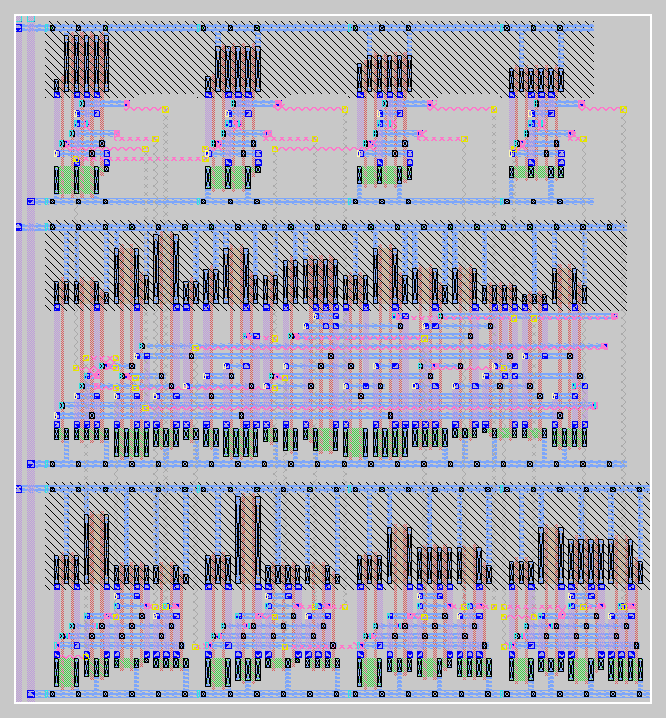
\includegraphics[width=\columnwidth]{figures/figures_magic_adder.png}\caption{Final 4-bit adder layout in MAGIC.}\end{figure}

\begin{figure}[H]\centering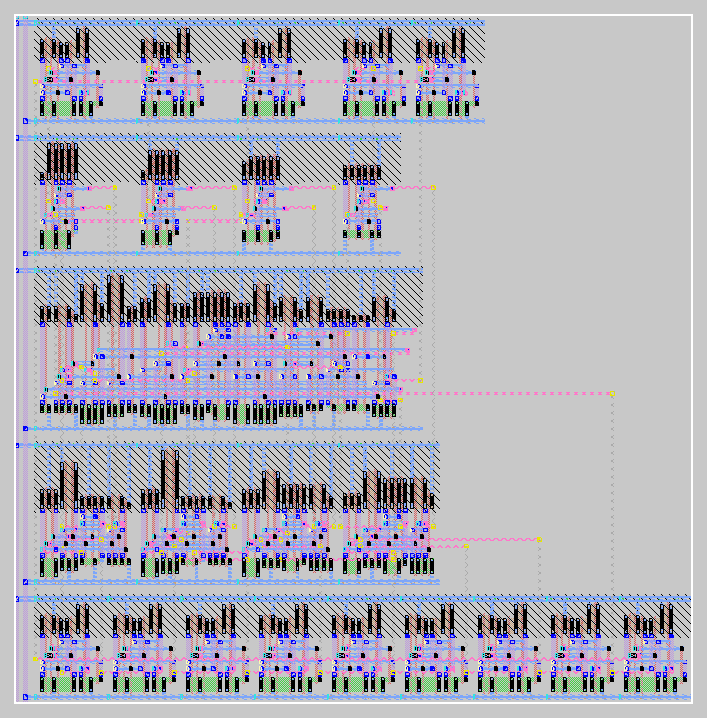
\includegraphics[width=\columnwidth]{figures/figures_magic_registered.png}\caption{Full registered circuit layout in MAGIC, with input and output flip-flops.}\end{figure}

\begin{table}[H]\centering\footnotesize
\caption{Layout results}
\begin{tabular}{|c|c|c|c|c|}\hline
Layout & DRC & LVS & Size ($\lambda$) & Area ($\mu$m$^2$) \\ \hline
Adder & 0 & match & 582x623 & 2936.9 \\ \hline
Registered & 0 & match & 925x935 & 7005.5 \\ \hline
\end{tabular}
\end{table}

The adder has 194 transistors and the registered circuit 348. Extracted wire capacitance is 376.9\,fF for the adder and 624.5\,fF for the registered circuit.

\section{Post-Layout Simulations and Delays}

\begin{figure*}[!t]\centering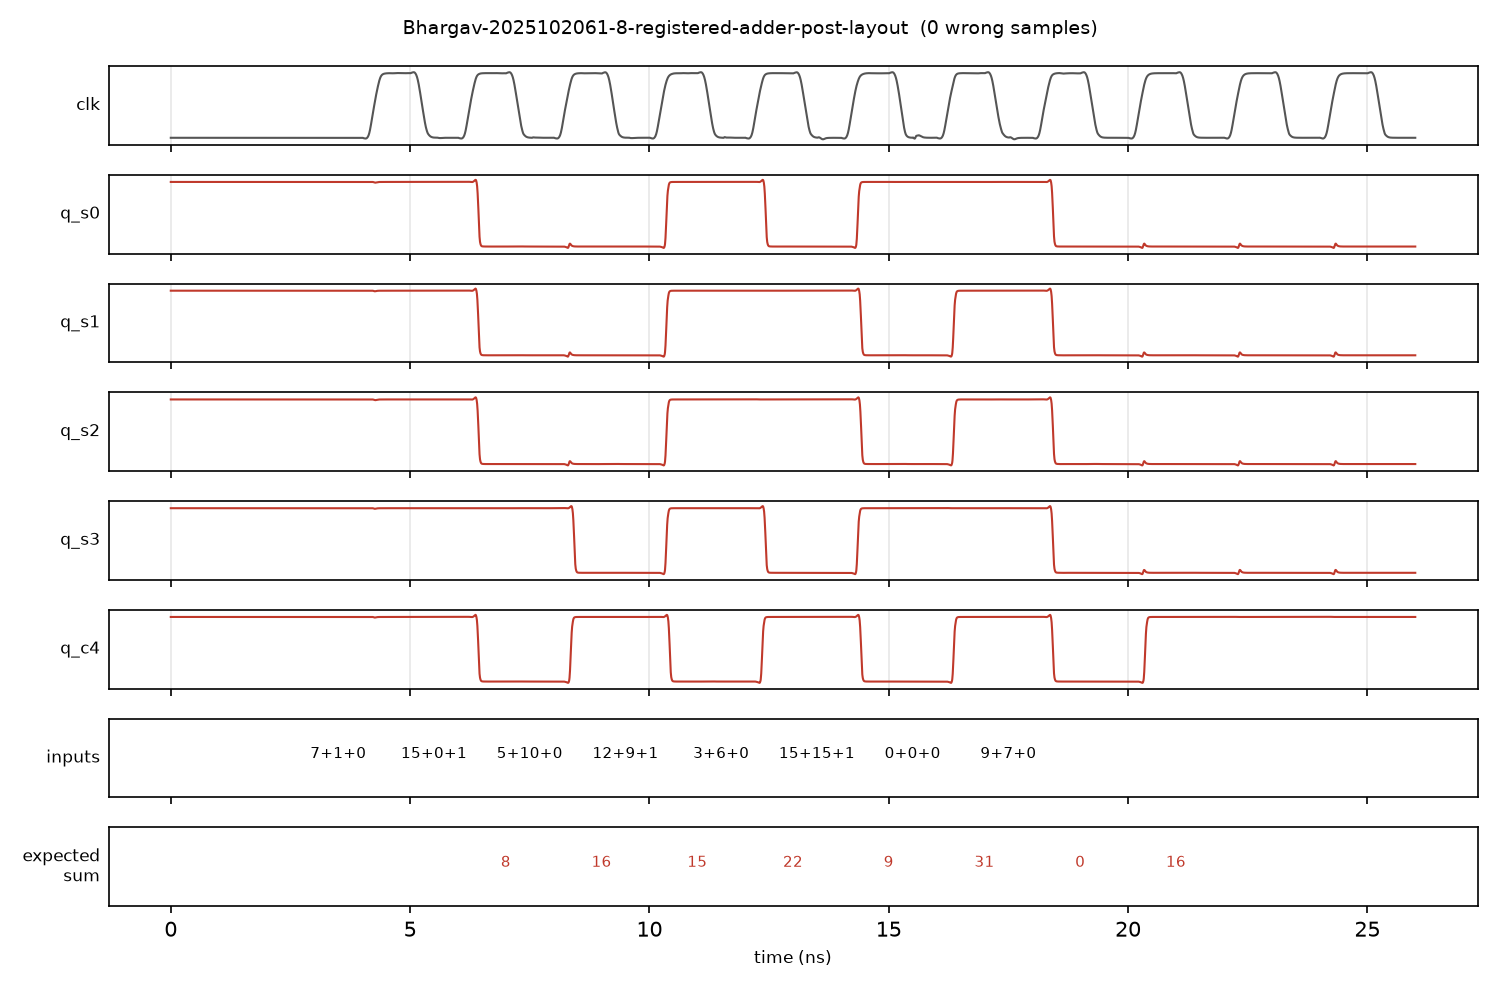
\includegraphics[width=0.9\textwidth]{figures/system_post-layout.png}\caption{Registered adder plot: post-layout. The outputs match the pre-layout run.}\end{figure*}

\subsection{Critical Path Delay}

\begin{table}[H]\centering\scriptsize
\caption{Course hint vector, $A = 1111$, $B = 0000$, $c_0$ toggling, post-layout}
\begin{tabular}{|c|c|c|c|}\hline
$c_0$ edge & Output & Type & Delay (ps) \\ \hline
rise & S0 & tpHL & 72.8 \\ \hline
rise & S1 & tpHL & 446.81 \\ \hline
rise & S2 & tpHL & 402.78 \\ \hline
rise & S3 & tpHL & 396.98 \\ \hline
rise & C4 & tpLH & 300.03 \\ \hline
fall & S0 & tpLH & 102.04 \\ \hline
fall & S1 & tpLH & 454.15 \\ \hline
fall & S2 & tpLH & 385.19 \\ \hline
fall & S3 & tpLH & 385.81 \\ \hline
fall & C4 & tpHL & 283.28 \\ \hline
\end{tabular}
\end{table}

\begin{figure}[H]\centering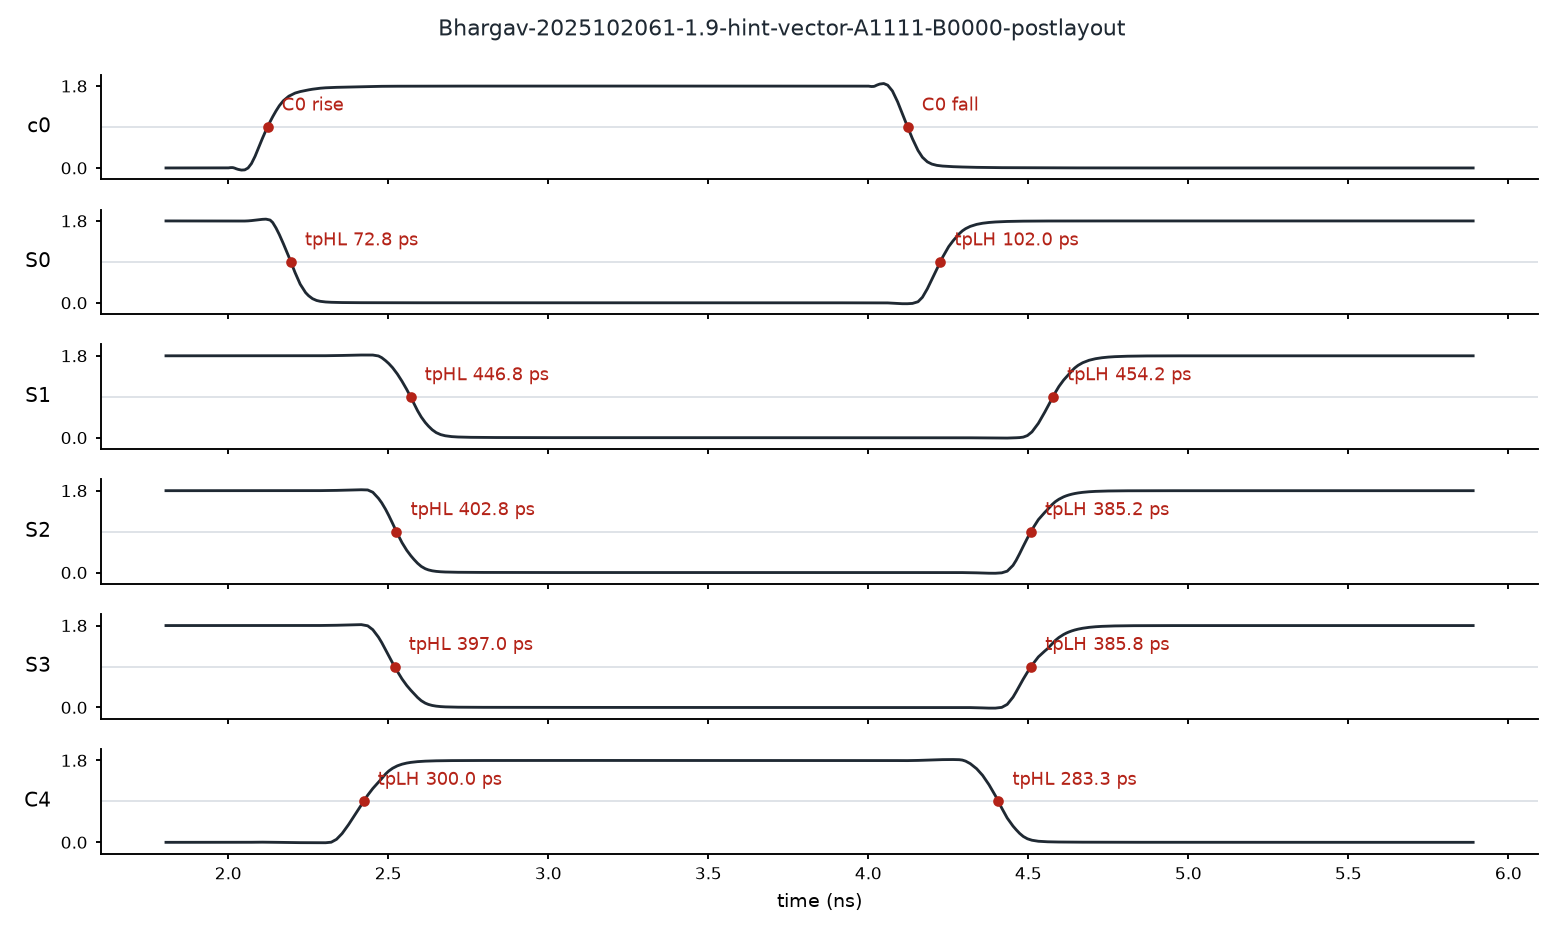
\includegraphics[width=\columnwidth]{figures/figures_hint_postlayout.png}\caption{Hint vector, extracted netlist, 50\% crossings marked.}\end{figure}

The slowest hint-vector output takes 454.1\,ps, but the search over all transitions finds a slower one: \textbf{579.88\,ps}, a1 rise to s3 rise, A=0001 B=0101 C0=0. When several inputs change together, a sample of 65520 transitions re-simulated on the extracted netlist gives \textbf{589.85\,ps}. This is taken as $t_{pd,max}$.

\begin{figure}[H]\centering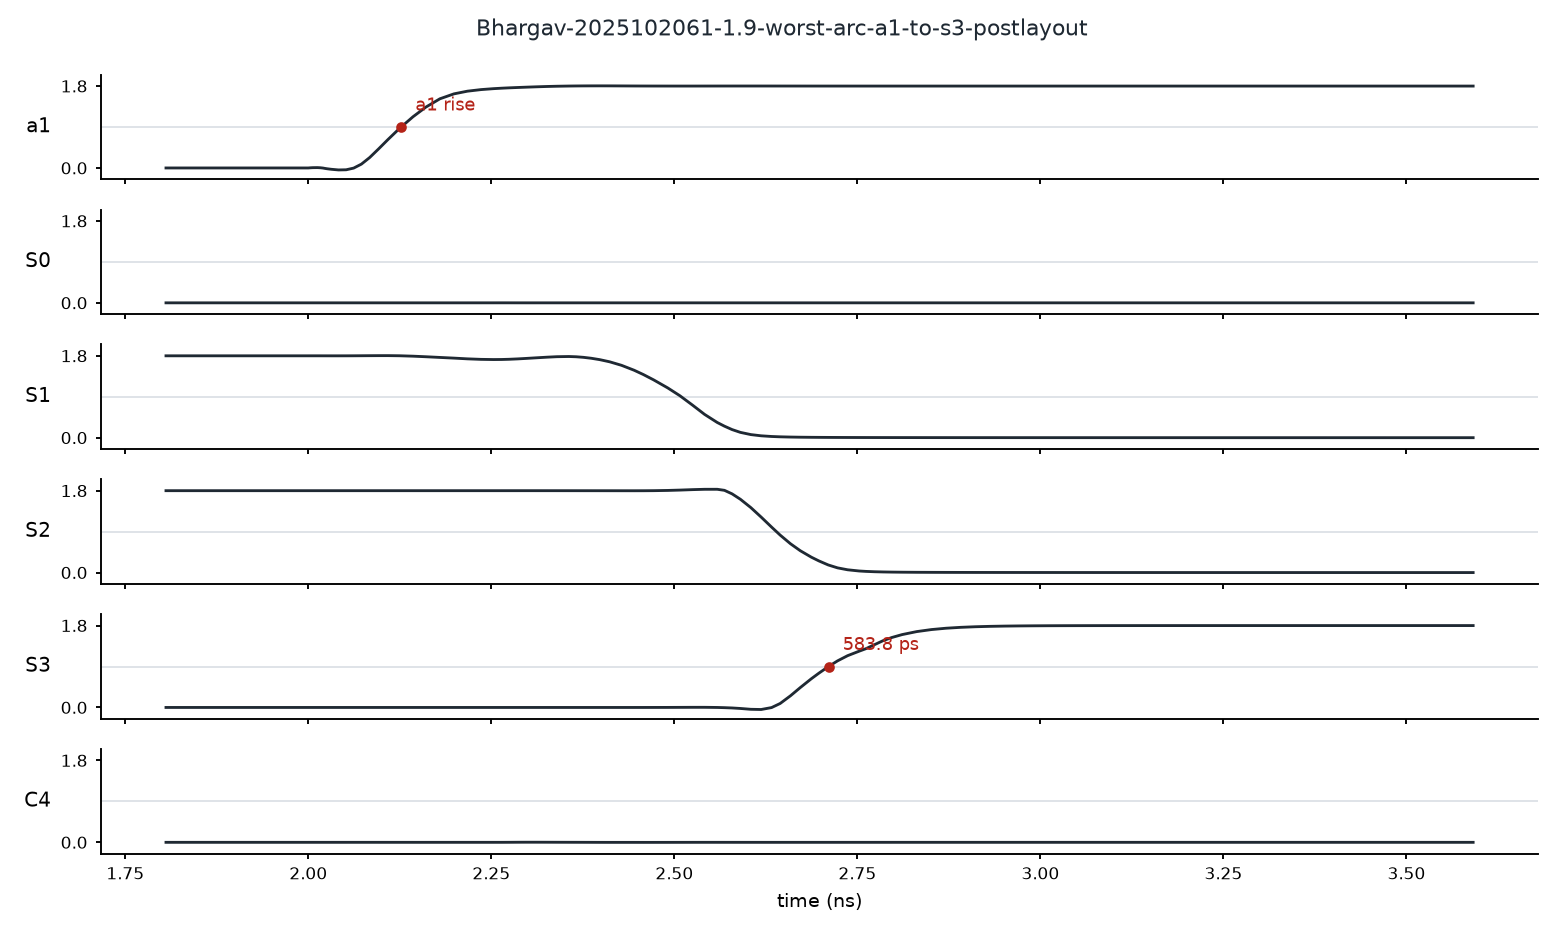
\includegraphics[width=\columnwidth]{figures/figures_worst_arc_postlayout.png}\caption{Worst single-input transition, extracted netlist.}\end{figure}

\subsection{Maximum Clock Frequency}
The course formula gives
\[ T = t_{pd,max} + t_{su} + t_{hold} = 589.85 + 38.0 + 45.7 = 673.6\,\text{ps}, \]
$f_{max} = 1.4847$\,GHz. At that clock the extracted registered circuit gave 264 wrong output samples, because the formula leaves out clock-to-Q. Using $T \ge t_{cq} + t_{pd,max} + t_{su} = 832.0$\,ps instead, and checking by simulation, the shortest clock that works is \textbf{872.1\,ps, 1.147\,GHz}.

\subsection{Power}
\[ P_{avg} = \frac{V_{DD}}{T_2 - T_1} \int_{T_1}^{T_2} I_{VDD}(t)\,dt \]
At the verified clock of 872.1\,ps, over 264 cycles of random and critical vectors, the circuit's own supply gives $P_{avg} = 3.3899$\,mW, so $PDP = P_{avg} \times t_{pd,max} = 1999.51$\,fJ. Input drivers, clock buffers and load inverters use a separate supply.

\begin{table}[H]\centering\footnotesize
\caption{Comparison of pre- and post-layout}
\label{tab:prepost}
\begin{tabular}{|c|c|c|}\hline
Parameter & Pre-Layout & Post-Layout \\ \hline
Worst single-input delay & 516.30 ps & 579.88 ps \\ \hline
Hint vector delay & 377.45 ps & 455.23 ps \\ \hline
$t_{cq}$ & 208.5 ps & 204.2 ps \\ \hline
$t_{su}$ & 34.0 ps & 38.0 ps \\ \hline
$t_{hold}$ & 55.1 ps & 45.7 ps \\ \hline
$T_{clk}(min)$, verified & 740.2 ps & 872.1 ps \\ \hline
$f_{clk}(max)$, verified & 1.351 GHz & 1.147 GHz \\ \hline
$P_{avg}$ at the post-layout clock & 3.0883 mW & 3.3899 mW \\ \hline
\end{tabular}
\end{table}

Post-layout delays are longer, by 12.3\% for the worst single-input delay, because the extracted netlist adds the capacitance of every wire and junction. Flip-flop clock-to-Q drops slightly after layout, because shared diffusion in the layout has less capacitance than the schematic's estimate.

\subsection{Layout Resistance}

MAGIC's resistance extraction crashed on this layout, so resistance was bounded instead: with the longest poly run's resistance in series with every gate, the worst delay rises by at most 3.61\%.

\section{Part II: SIMD-Reconfigurable 8-bit Adder}
GPUs often split one wide datapath into narrower sub-words~\cite{hp}. Here two copies of the Part I adder, CLA0 for bits 3..0 and CLA1 for bits 7..4, form an 8-bit adder with a control input SIMD\_MODE:
\begin{itemize}
\item SIMD\_MODE $= 0$: CLA0's carry-out goes into CLA1's carry-in, one 8-bit add.
\item SIMD\_MODE $= 1$: the inter-block carry is forced to 0, two independent 4-bit adds.
\end{itemize}
The cost of this is measured against a \emph{baseline}: the same two adders wired directly, with no gating.

\subsection{Architecture}

The block diagram below shows the two Part I adders and the carry-gating cell between them. CLA0's carry-out, c4lo, is also an output, because in dual mode it is the carry of the lower 4-bit result; it drives the same 20$\lambda$/10$\lambda$ load as the other outputs. The baseline is the same diagram without the gate, with c4lo wired straight to CLA1's carry-in.

\begin{figure*}[!t]\centering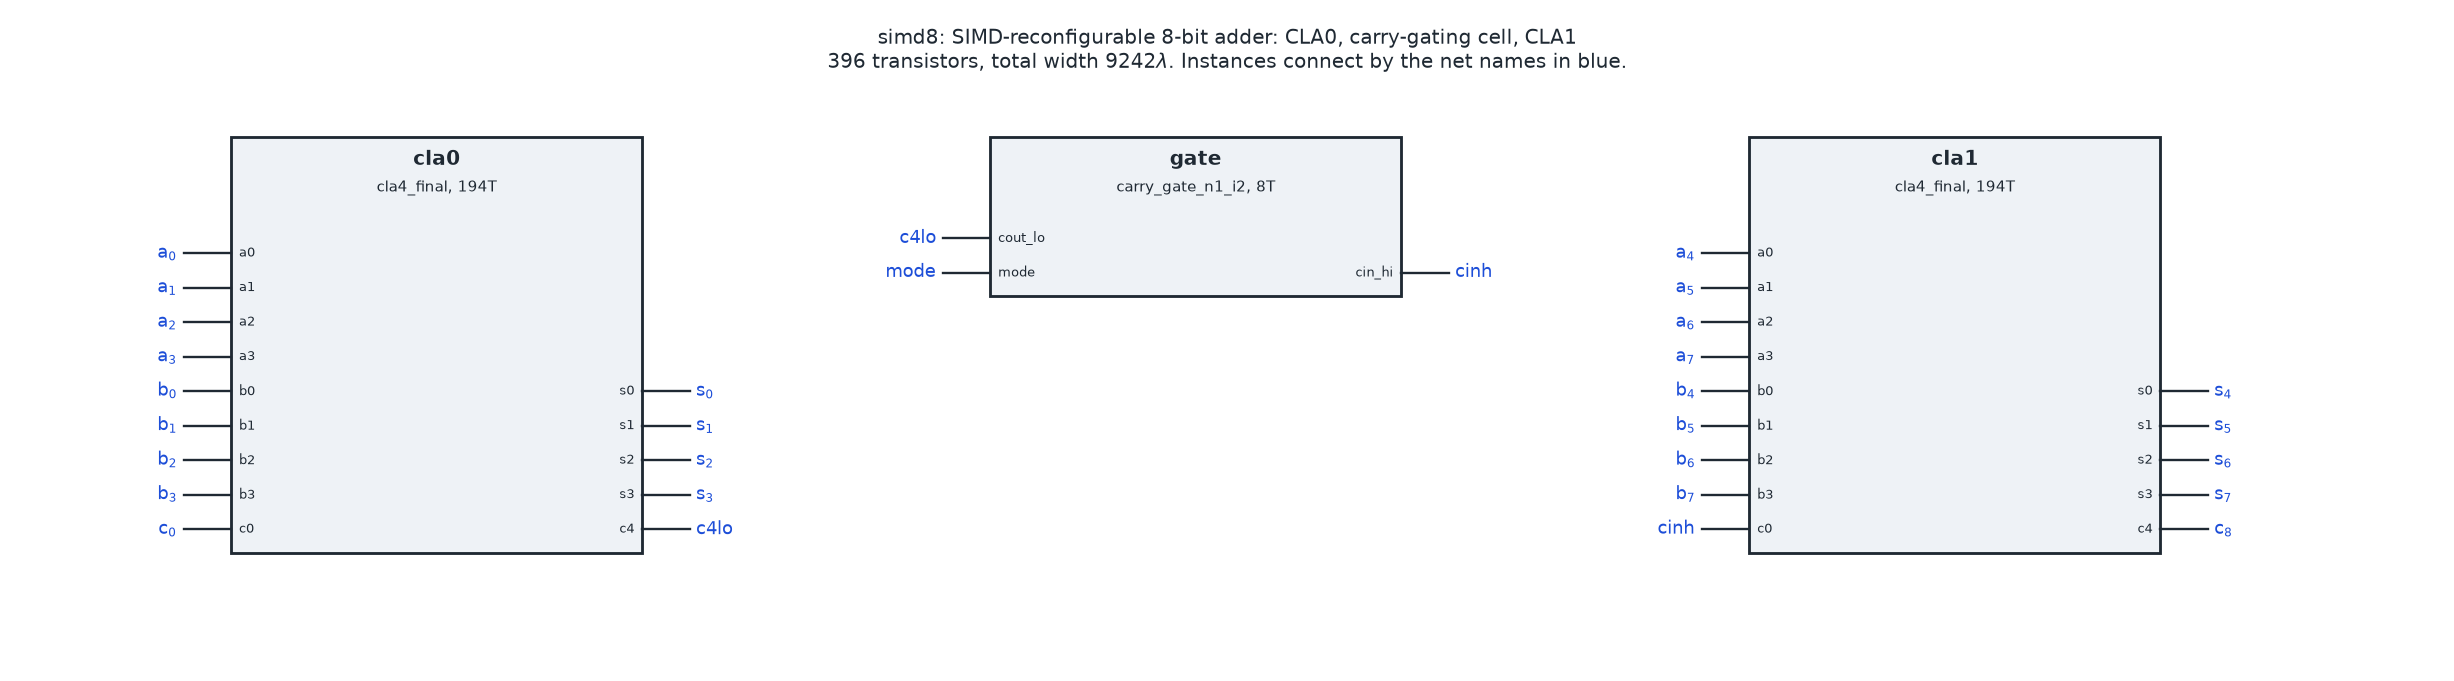
\includegraphics[width=0.95\textwidth]{figures/figures_2.0a_simd8-blocks.png}\caption{SIMD 8-bit adder: CLA0, the carry-gating cell and CLA1. c4lo is CLA0's carry-out and cinh CLA1's carry-in.}\end{figure*}

\subsection{Carry-Gating Cell}
\[ c_{in,hi} = c_{out,lo} \cdot \overline{\mathrm{SIMD\_MODE}} \]
This is an AND gate. In static CMOS the cell is a NAND2 followed by an inverter on the carry path, with a unit inverter making $\overline{\mathrm{SIMD\_MODE}}$; the mode is held during an add, so that inverter is off the timing path. The cell has 8 transistors.

\begin{figure}[H]\centering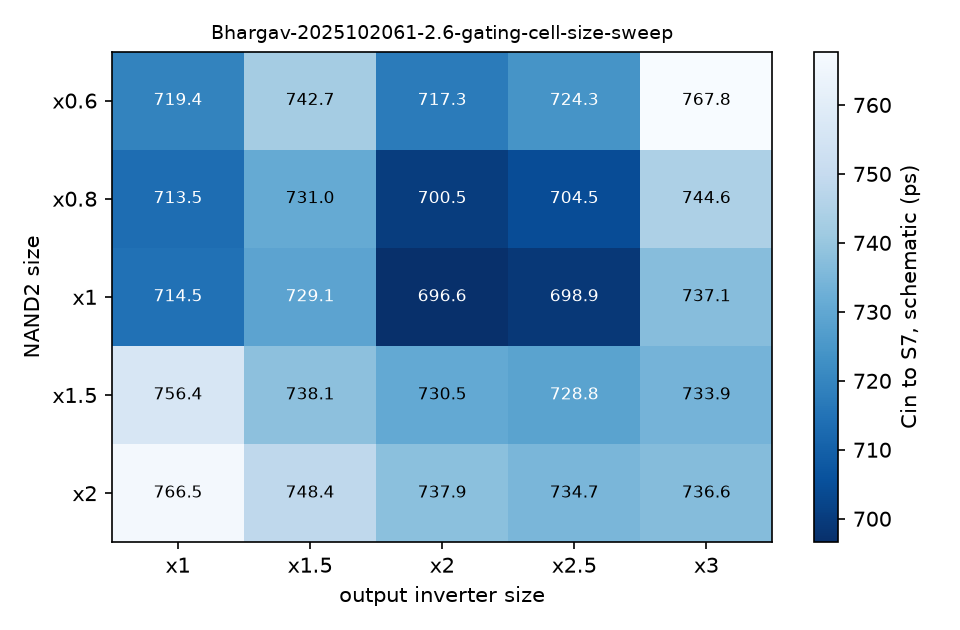
\includegraphics[width=\columnwidth]{figures/figures_2.6_gating-cell-size-sweep.png}\caption{Gate sizing sweep, Cin to S7 in mode 0, schematic. Best: NAND2 x1, inverter x2.}\end{figure}

\begin{figure}[H]\centering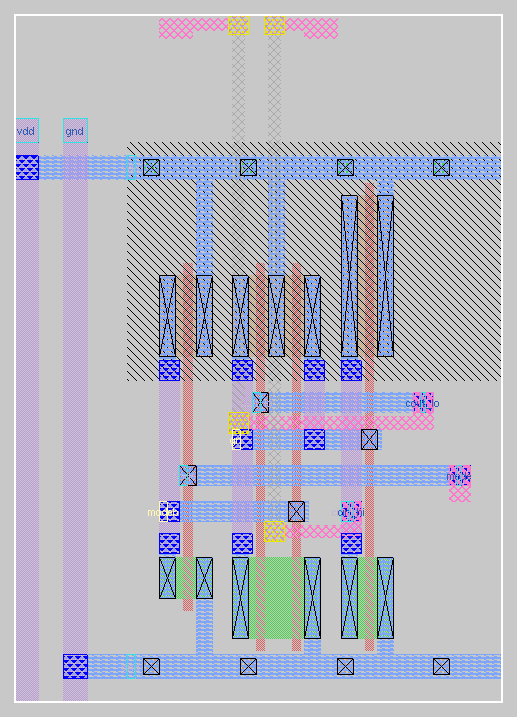
\includegraphics[width=0.6\columnwidth]{figures/figures_magic_gate.png}\caption{MAGIC layout of the carry-gating cell, with carry pads above it.}\end{figure}

\begin{table}[H]\centering\footnotesize
\caption{Carry-gating cell alone, cout\_lo to cin\_hi with the 20/10$\lambda$ load}
\begin{tabular}{|c|c|c|c|}\hline
View & Worst & Rising & Falling \\ \hline
Pre-layout & 104.27 & 89.12 & 104.27 \\ \hline
Post-layout & 110.46 & 95.2 & 110.46 \\ \hline
\end{tabular}
\end{table}

\subsection{Layout}
The Part I adder was laid out again with two extra metal 3 pads above its top row, for $c_4$ and $c_0$. The 8-bit layout places this cell twice, with the gating cell between the copies in the SIMD design, and joins the inter-block carries on metal 5, which no cell uses. A first attempt that placed all gates of both adders in one set of rows ran out of routing tracks.

\begin{figure*}[!t]\centering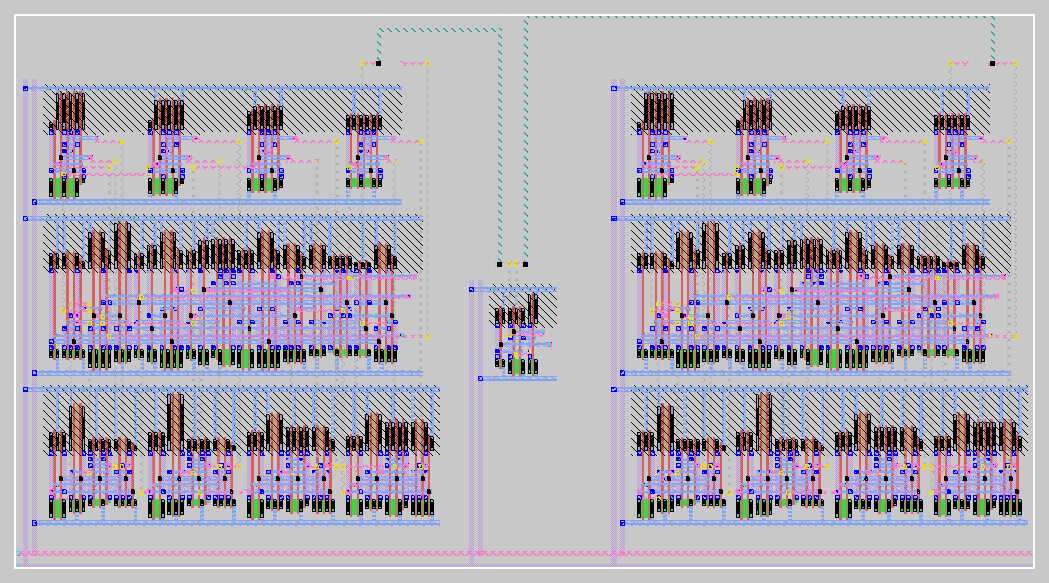
\includegraphics[width=0.95\textwidth]{figures/figures_magic_simd8.png}\caption{SIMD 8-bit adder in MAGIC: CLA0, the gating cell and CLA1. The dashed lines at the top are metal 5.}\end{figure*}

\begin{figure}[H]\centering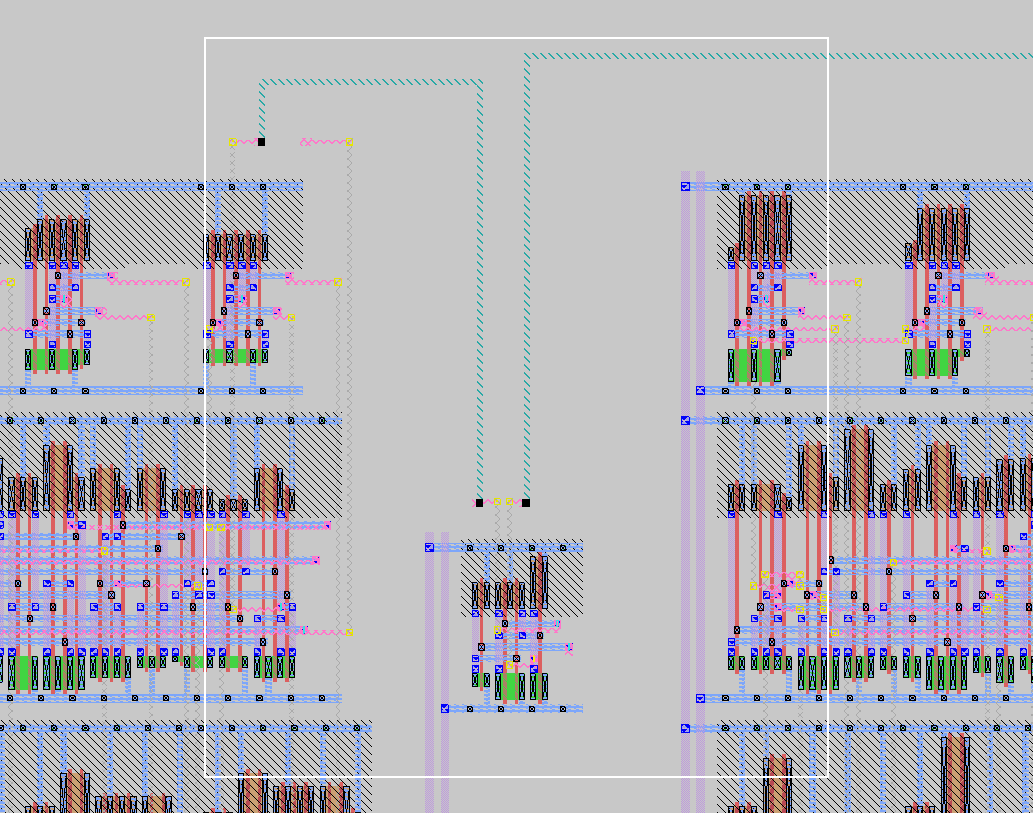
\includegraphics[width=\columnwidth]{figures/figures_magic_simd8_gate_zoom.png}\caption{Close-up in MAGIC: the gating cell between the two adders, with its two metal 5 carries.}\end{figure}

\begin{figure}[H]\centering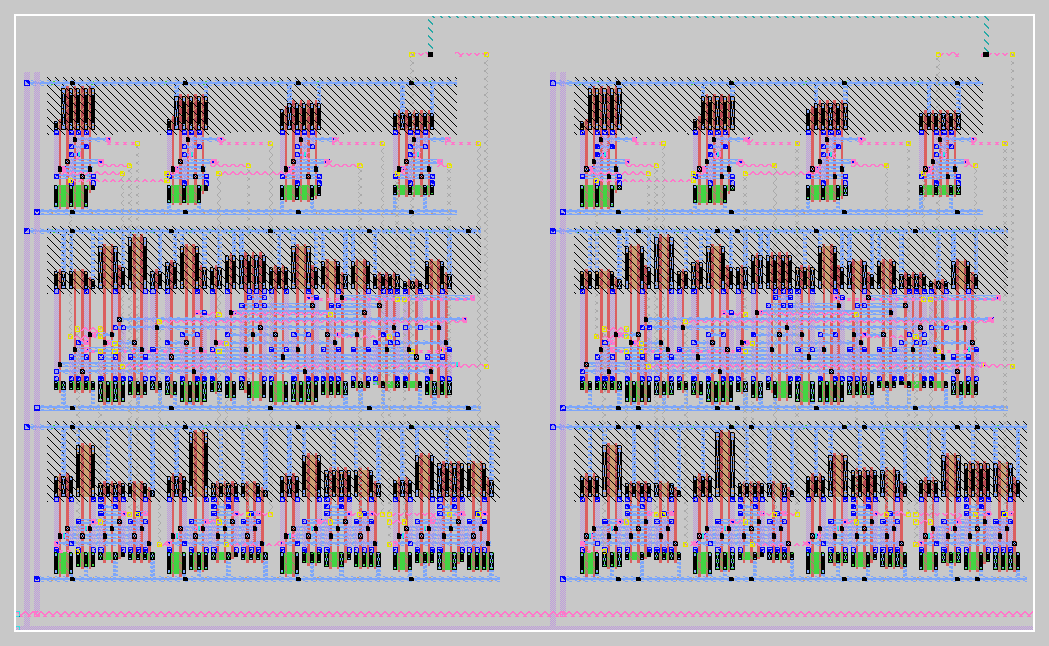
\includegraphics[width=\columnwidth]{figures/figures_magic_base8.png}\caption{Baseline 8-bit adder in MAGIC: c4lo runs on metal 5 straight from CLA0 to CLA1.}\end{figure}

\begin{table}[H]\centering\footnotesize
\caption{Part II layout results}
\begin{tabular}{|c|c|c|c|}\hline
Design & DRC & Devices (LVS) & Area ($\mu$m$^2$) \\ \hline
Baseline & 0 & 388, match & 7749.0 \\ \hline
SIMD & 0 & 396, match & 8858.7 \\ \hline
\end{tabular}
\end{table}

\subsection{Worst-Case Delay in Both Modes}
The search runs 13,312 single-input transitions per case: every transition of CLA0's nine inputs with CLA1 set to pass a carry through all four bits, and every transition of CLA1's eight inputs with CLA0's carry-out held at 0 and at 1.

\begin{table}[H]\centering\footnotesize
\caption{Worst-case propagation delay}
\begin{tabular}{|c|c|c|}\hline
Case & Pre-layout (ps) & Post-layout (ps) \\ \hline
Baseline & 855.22 & 1030.86 \\ \hline
SIMD, mode 0 & 920.09 & 1109.77 \\ \hline
SIMD, mode 1 & 516.31 & 570.22 \\ \hline
\end{tabular}
\end{table}

\begin{figure*}[!t]\centering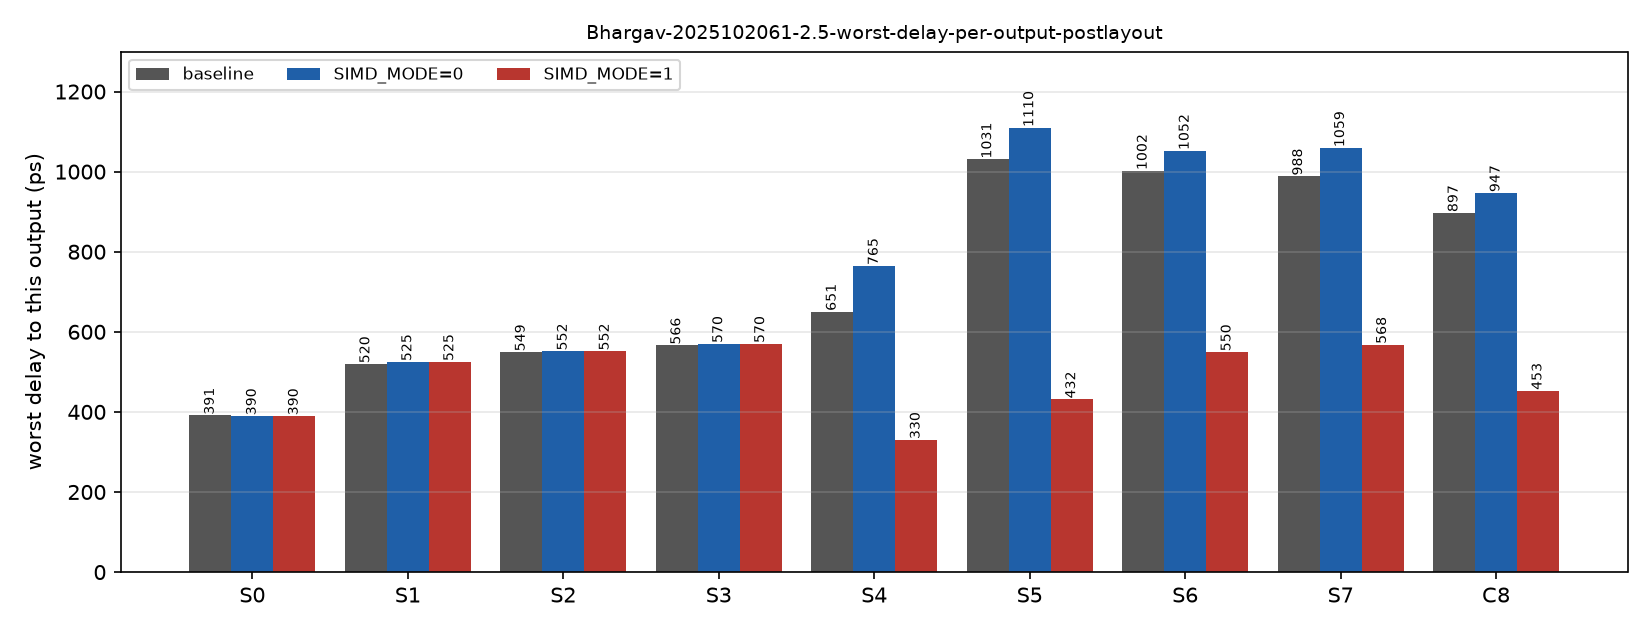
\includegraphics[width=0.85\textwidth]{figures/figures_2.5_worst-delay-per-output-postlayout.png}\caption{Worst post-layout delay to each output.}\end{figure*}

In mode 0 the worst path is a3 fall to S5, through CLA0's carry tree and the gating cell into CLA1. In mode 1 the carry never crosses, so the worst path stays inside one 4-bit block.

\subsection{Delay Penalty}
Worst-case carry vector $A = $ 0xFF, $B = $ 0x00, $c_{in,0}$ toggling, delay from $c_{in,0}$ to $S_7$:
\[ \text{Delay penalty} = \frac{t_{pd,SIMD} - t_{pd,baseline}}{t_{pd,baseline}} \times 100\% \]

\begin{table}[H]\centering\footnotesize
\caption{Cin to S7 on the worst-case vector}
\begin{tabular}{|c|c|c|c|}\hline
View & Baseline (ps) & SIMD m0 (ps) & Penalty \\ \hline
Pre-layout & 633.33 & 691.62 & +58.28 ps, 9.20\% \\ \hline
Post-layout & 816.11 & 877.83 & +61.72 ps, 7.56\% \\ \hline
\end{tabular}
\end{table}

\begin{figure*}[!t]\centering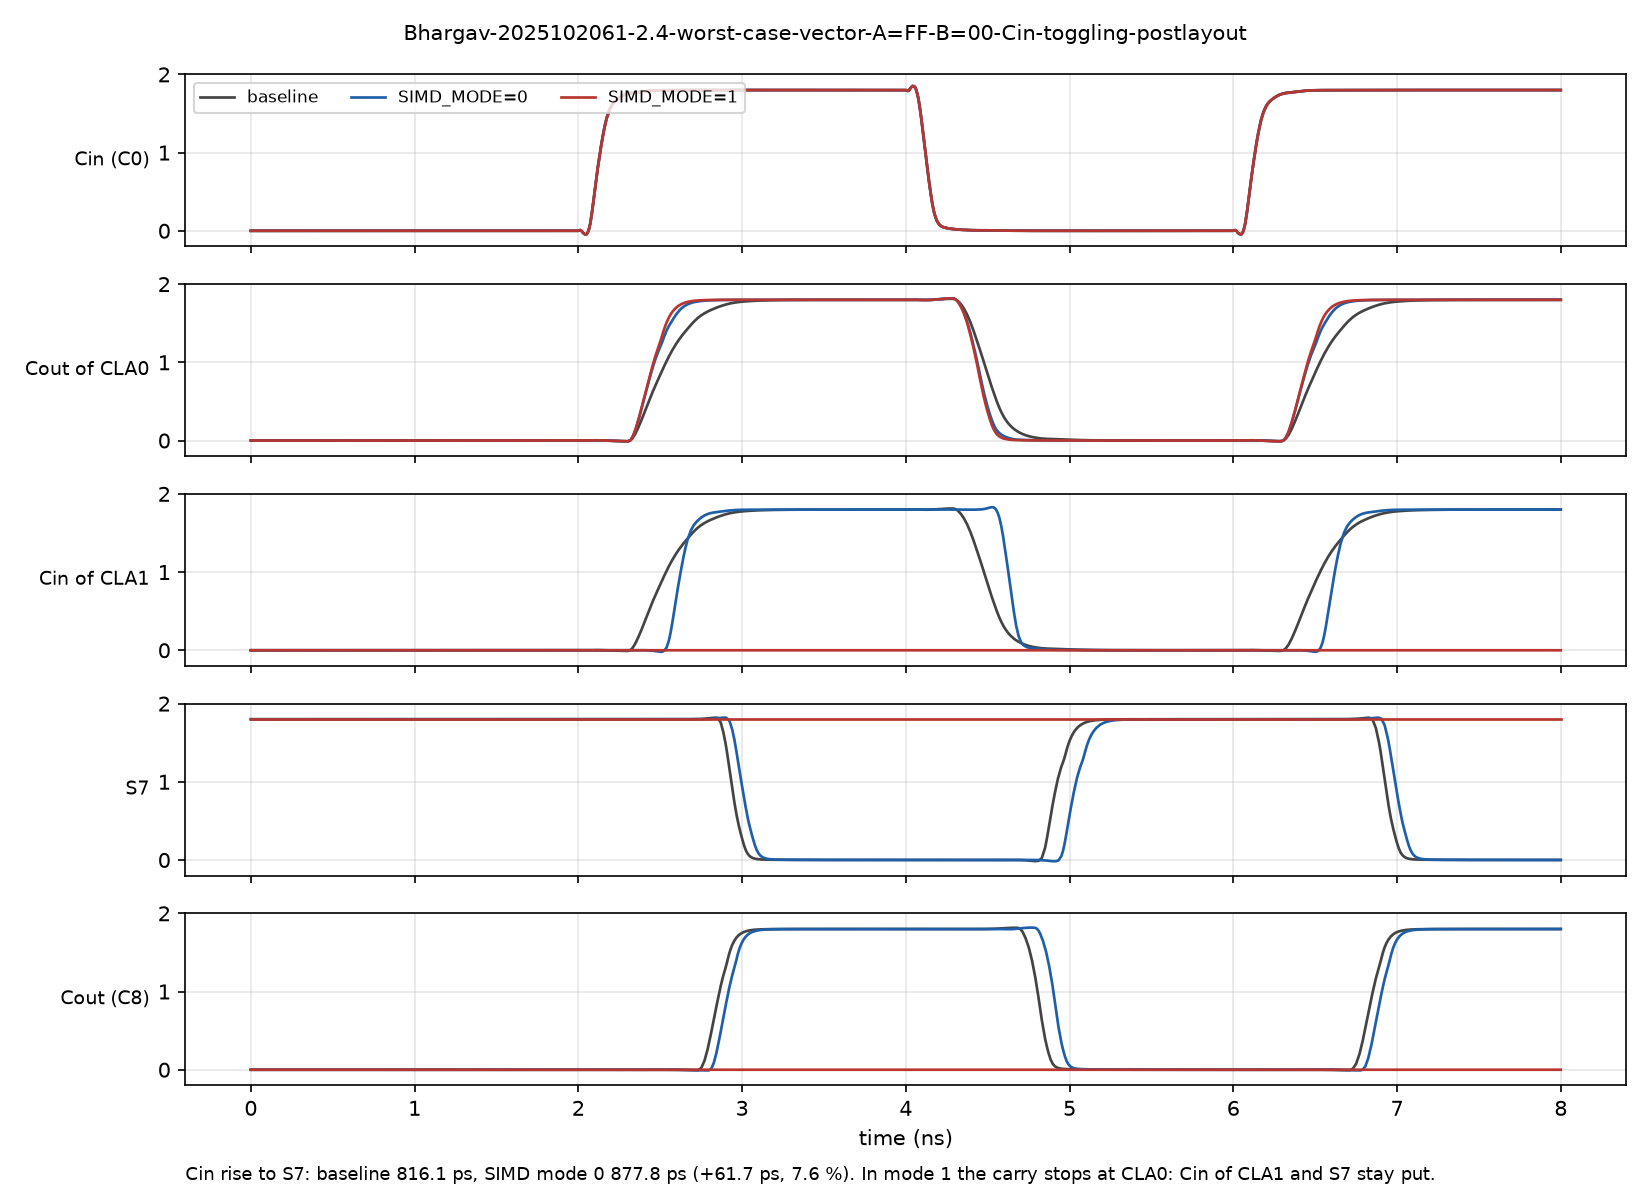
\includegraphics[width=0.8\textwidth]{figures/figures_2.4_worst-case-vector-postlayout.png}\caption{Post-layout waveforms on the worst-case vector. In mode 1 CLA1's carry-in stays at 0.}\end{figure*}

The gate alone takes 110.46\,ps, but the penalty is only 61.72\,ps: in the baseline, CLA0's carry-out drives CLA1's carry-in load directly, while in the SIMD design the gate isolates that load, so CLA0's carry-out switches sooner.

\subsection{Power Penalty}
Course-formula $f_{max}$, with the Part I flip-flop's post-layout $t_{su}$ and $t_{hold}$: baseline 0.897\,GHz, SIMD mode 0 0.838\,GHz, mode 1 1.529\,GHz. At those clocks some random vectors that change several inputs at once did not settle, so the shortest clock at which all three cases settle on the same 200 random vectors was found: 1400\,ps. Power is compared there, with identical inputs for all three.
\[ \text{Power penalty} = \frac{P_{SIMD,0} - P_{baseline}}{P_{baseline}} \times 100\% \]

\begin{table}[H]\centering\footnotesize
\caption{Average power at 1400 ps, post-layout}
\begin{tabular}{|c|c|c|}\hline
Case & 10 cycles ($\mu$W) & 200 vectors ($\mu$W) \\ \hline
Baseline & 1695.2 & 1876.3 \\ \hline
SIMD, mode 0 & 1720.7 & 1919.5 \\ \hline
SIMD, mode 1 & 1592.4 & 1713.7 \\ \hline
\end{tabular}
\end{table}

Power penalty in 8-bit mode: \textbf{1.50\%} over 10 cycles, and 2.30\% over 200 vectors.

\subsection{Energy-Delay Product}
\[ EDP = P_{avg} \times t_{pd}^2 \]

\begin{table}[H]\centering\footnotesize
\caption{Energy-delay product, post-layout}
\begin{tabular}{|c|c|c|c|}\hline
Case & $P_{avg}$ ($\mu$W) & $t_{pd,max}$ (ps) & EDP (J s) \\ \hline
Baseline & 1695.2 & 1030.86 & 1.801e-21 \\ \hline
SIMD, mode 0 & 1720.7 & 1109.77 & 2.119e-21 \\ \hline
SIMD, mode 1 & 1592.4 & 570.22 & 5.178e-22 \\ \hline
\end{tabular}
\end{table}

\begin{table}[H]\centering\footnotesize
\caption{Cost of reconfigurability, SIMD mode 0 against the baseline, post-layout}
\begin{tabular}{|c|c|}\hline
Measure & Penalty \\ \hline
Cin to S7 delay & 7.56\% \\ \hline
$t_{pd,max}$ & 7.65\% \\ \hline
Power, 10 cycles & 1.50\% \\ \hline
EDP & 17.6\% \\ \hline
Transistors & +8 \\ \hline
Area & 14.3\% \\ \hline
\end{tabular}
\end{table}

Delay counts twice in EDP, so the delay penalty dominates the small power penalty. In dual mode each add is only 4 bits long, so its EDP is far lower.

\section{Verilog HDL}
\emph{To be completed in the next draft, with Part III: behavioural Verilog of the 4-bit CLA and the SIMD adder, test vectors for every mode, and annotated simulation waveforms.}

\section{FPGA Implementation}
\emph{To be completed in the next draft, with Part III: synthesis and implementation on the Boolean Board, test scenarios, and oscilloscope captures.}

\section*{Acknowledgment}
I thank Prof. Abhishek Srivastava for the course and this project, and the teaching assistants for their guidance.

\begin{thebibliography}{9}
\bibitem{miao} J. Miao and S. Li, ``A novel implementation of 4-bit carry look-ahead adder,'' in \emph{Proc. IEEE EDSSC}, 2017.
\bibitem{yuan} J. Yuan and C. Svensson, ``High-speed CMOS circuit technique,'' \emph{IEEE J. Solid-State Circuits}, vol. 24, no. 1, pp. 62--70, 1989.
\bibitem{stoj} V. Stojanovi\'c and V. G. Oklobd\v{z}ija, ``Comparative analysis of master-slave latches and flip-flops for high-performance and low-power systems,'' \emph{IEEE J. Solid-State Circuits}, vol. 34, no. 4, pp. 536--548, 1999.
\bibitem{hp} J. L. Hennessy and D. A. Patterson, \emph{Computer Architecture: A Quantitative Approach}.
\end{thebibliography}
\end{document}
